\documentclass[a4paper,oneside]{book}
\usepackage[top=2.54cm, bottom=2.54cm, left=3.17cm, right=3.17cm]{geometry}
\usepackage[spanish,es-tabla]{babel} % Traduce cuadros por tablas
% La siguiente linea es para que se reconozcan los acentos.
% Si falla probar con la siguiente
\usepackage[utf8]{inputenc}
\usepackage[T1]{fontenc}
\usepackage{graphicx}
\graphicspath{ {Imagenes/} }
\DeclareGraphicsExtensions{.png,.jpg}
\setlength{\parindent}{12pt}
\setcounter{secnumdepth}{3}
\usepackage{fancyhdr}
\pagestyle{fancy}
\fancyhf{}
\chead{Sistema de gestión de mueblería}
\lfoot{\leftmark}
\rfoot{\thepage}
\usepackage{titlesec}
% \setcounter{tocdepth}{3} para que aparezcan las subsecciones en el indice https://www.lawebdelprogramador.com/foros/TeX-Latex/619886-subsubsection.html
% \usepackage[latin1]{inputenc}
\usepackage[none]{hyphenat}
\usepackage[
pdfauthor={Nicolás Bachs, Loïk Choua},
pdftitle={Sistema de Gestión de mueblería},
pageanchor,
hidelinks,
plainpages=false,
pdfpagelabels,
hypertexnames=false,
unicode	]{hyperref}
% Poner links en el proyecto
% \url{http://www.latex-project.org/}
% \href{http://www.latex-project.org/}{latex project}
\usepackage{wrapfig}
\usepackage{lscape}
\usepackage{rotating}
\usepackage{epstopdf}
\usepackage{multirow, array}
\usepackage{array,longtable}
\usepackage{float}
\usepackage[table,xcdraw]{xcolor}
\usepackage[euler]{textgreek}
\usepackage{makecell}
\usepackage{caption}
% Comandos para los diagramas de actividad
\newcommand{\activityDiagram}[2]{
	\begin{figure}[H]
		\centering
		\includegraphics[width=\textwidth,height=0.95\textheight,keepaspectratio]{DiagramasActividad/DiagramaDeActividad/#1}
		\caption{#2}
	\label{fig:#1}
	\end{figure}
}

% Comandos para los diagramas de estado
\newcommand{\stateDiagram}[2]{
	\begin{figure}[H]
		\centering
		\includegraphics[width=\textwidth,height=0.95\textheight,keepaspectratio]{DiagramaDeEstado/#1}
		\caption{#2}
	\label{fig:#1}
	\end{figure}
}


% Cargar imagen de escenario
% Parámetro 1: nombre de imagen - Parámetro 2: epígrafe
\newcommand{\stageImage}[2]{
	\begin{figure}[H]
		\centering
		\includegraphics[width=\textwidth,height=0.35\textheight,keepaspectratio]{escenarios/#1}
		\caption{#2}
	\label{fig:#1}
	\end{figure}
}

\newcommand{\stageTitle}[2]{
	\noindent\begin{minipage}{\textwidth}
	{#2}
	\stageImage{#1}{#2}
	\end{minipage}
}

\newcommand{\stageTitleD}[3]{
	\noindent\begin{minipage}{\textwidth}
	{#3}
	\begin{figure}[H]
		\centering
		\includegraphics[width=\textwidth,height=0.35\textheight,keepaspectratio]{escenarios/#1}
	\end{figure}
	\begin{figure}[H]
		\centering
		\includegraphics[width=\textwidth,height=0.35\textheight,keepaspectratio]{escenarios/#2}
		\caption{#3}
	\label{fig:#1}
	\end{figure}
	\end{minipage}
	}

% Comandos para numerar los escenarios
% Ejemplo de uso: \stageLogin{00} --> AI_01_00
\newcommand{\stageLogin}[1]{\hyperref[fig:login]{AI\_01\_#1}}
\newcommand{\stageMain}[1]{\hyperref[fig:main]{AI\_02\_#1}}
\newcommand{\stageHeader}[1]{\hyperref[fig:header]{AI\_03\_#1}}
\newcommand{\stageAlarms}[1]{\hyperref[fig:alarms]{AI\_04\_#1}}
\newcommand{\stageCommunicationErrors}[1]{\hyperref[fig:communicationErrors]{AI\_05\_#1}}
\newcommand{\stageSitesMap}[1]{\hyperref[fig:sitesMap]{AI\_06\_#1}}
\newcommand{\stageFilters}[1]{\hyperref[fig:filters]{AI\_07\_#1}}

\newcommand{\stageDashboard}[1]{\hyperref[fig:dashboard]{AI\_08\_#1}}
\newcommand{\stageManagement}[1]{\hyperref[fig:management]{AI\_09\_#1}}

\newcommand{\stageSiteData}[1]{\hyperref[fig:siteData]{AI\_10\_#1}}
\newcommand{\stageSiteLocation}[1]{\hyperref[fig:siteLocation]{AI\_11\_#1}}
\newcommand{\stageSiteComponent}[1]{\hyperref[fig:siteComponent]{AI\_12\_#1}}
\newcommand{\stageChannel}[1]{{AI\_13\_#1}}
\newcommand{\stageAdministration}[1]{{AI\_14\_#1}}

\newcommand{\stageComponentConfig}[1]{\hyperref[fig:componentConfig]{AI\_15\_#1}}
\newcommand{\stageRequestConfig}[1]{\hyperref[fig:requestConfig]{AI\_16\_#1}}
\newcommand{\stageInputConfig}[1]{\hyperref[fig:inputConfig]{AI\_17\_#1}}
\newcommand{\stageSiteConfig}[1]{\hyperref[fig:siteConfig]{AI\_18\_#1}}
\newcommand{\stageUnifilarConfig}[1]{\hyperref[fig:unifilarConfig]{AI\_19\_#1}}
\newcommand{\stageUnifilarConfigOp}[1]{\hyperref[fig:unifilarConfigOp]{AI\_20\_#1}}
\newcommand{\stageUnifilarConfigOpInputs}[1]{\hyperref[fig:unifilarConfigOpInputs]{AI\_21\_#1}}
\newcommand{\stageUnifilarConfigOpRequests}[1]{\hyperref[fig:unifilarConfigOpRequests]{AI\_22\_#1}}
\newcommand{\stageUnifilarConfigOpStates}[1]{\hyperref[fig:unifilarConfigOpStates]{AI\_23\_#1}}

\newcommand{\stageUserData}[1]{\hyperref[fig:userData]{AI\_24\_#1}}
\newcommand{\stageUserSite}[1]{\hyperref[fig:userSite]{AI\_25\_#1}}
\newcommand{\stageProfile}[1]{\hyperref[fig:profile]{AI\_26\_#1}}

\newcommand{\stageChannelCommunication}[1]{\hyperref[fig:channelCommunication]{AI\_27\_#1}}

\newcommand{\stageUnifilar}[1]{\hyperref[fig:unifilar]{AI\_28\_#1}}
\newcommand{\stageDevices}[1]{\hyperref[fig:devices]{AI\_29\_#1}}
\newcommand{\stageSiteRequests}[1]{\hyperref[fig:requestsSite]{AI\_30\_#1}}
\newcommand{\stageAnalogInputs}[1]{\hyperref[fig:analog]{AI\_31\_#1}}
\newcommand{\stageDigitalInputs}[1]{\hyperref[fig:digital]{AI\_32\_#1}}
\newcommand{\stageCommands}[1]{\hyperref[fig:commands]{AI\_33\_#1}}
\newcommand{\stageRequests}[1]{\hyperref[fig:requests]{AI\_34\_#1}}
\newcommand{\stageTasks}[1]{\hyperref[fig:tasks]{AI\_35\_#1}}

\newcommand{\stageHistory}[1]{{UI\_36\_#1}}

\newcommand{\stageName}[2]{Escenario #1 : #2}
\newcommand{\stageLoginName}{\stageName{\stageLogin{00}}{Inicio de sesión}}
\newcommand{\stageHeaderName}{\stageName{\stageHeader{00}}{Encabezado del sistema}}
\newcommand{\stageMainName}{\stageName{\stageMain{00}}{Vista principal}}
\newcommand{\stageAlarmsName}{\stageName{\stageAlarms{00}}{Alarmas}}
\newcommand{\stageCommunicationErrorsName}{\stageName{\stageCommunicationErrors{00}}{Errores de comunicación}}
\newcommand{\stageSitesMapName}{\stageName{\stageSitesMap{00}}{Mapa de sitios}}
\newcommand{\stageFiltersName}{\stageName{\stageFilters{00}}{Filtros de mapa}}

\newcommand{\stageDashboardName}{\stageName{\stageDashboard{00}}{Panel de control}}
\newcommand{\stageManagementName}{\stageName{\stageManagement{00}}{Gestión de entidades}}
\newcommand{\stageSiteDataName}{\stageName{\stageSiteData{00}}{Sitios - Datos generales}}
\newcommand{\stageSiteLocationName}{\stageName{\stageSiteLocation{00}}{Sitios - Ubicación}}
\newcommand{\stageSiteComponentName}{\stageName{\stageSiteComponent{00}}{Sitios - Configuración de componentes}}
\newcommand{\stageUserDataName}{\stageName{\stageUserData{00}}{Usuarios - Datos generales}}
\newcommand{\stageUserSiteName}{\stageName{\stageUserSite{00}}{Usuarios - Asignación de sitios}}
\newcommand{\stageProfileName}{\stageName{\stageProfile{00}}{Perfiles}}

\newcommand{\stageComponentConfigName}{\stageName{\stageComponentConfig{00}}{Configuración de componentes - Datos generales}}
\newcommand{\stageRequestConfigName}{\stageName{\stageRequestConfig{00}}{Configuración de componentes - Pedidos}}
\newcommand{\stageInputConfigName}{\stageName{\stageInputConfig{00}}{Configuración de componentes - Entradas}}
\newcommand{\stageSiteConfigName}{\stageName{\stageSiteConfig{00}}{Configuración de sitios - Datos generales}}
\newcommand{\stageUnifilarConfigName}{\stageName{\stageUnifilarConfig{00}}{Configuración de sitios - Creación de diagrama unifilar}}
\newcommand{\stageUnifilarConfigOpName}{\stageName{\stageUnifilarConfigOp{00}}{Configuración de diagrama unifilar}}
\newcommand{\stageUnifilarConfigOpInputsName}{\stageName{\stageUnifilarConfigOpInputs{00}}{Configuración de diagrama unifilar - Entradas}}
\newcommand{\stageUnifilarConfigOpRequestsName}{\stageName{\stageUnifilarConfigOpRequests{00}}{Configuración de diagrama unifilar - Pedidos}}
\newcommand{\stageUnifilarConfigOpStatesName}{\stageName{\stageUnifilarConfigOpStates{00}}{Configuración de diagrama unifilar - Estados de dispositivos}}
\newcommand{\stageChannelCommunicationName}{\stageName{\stageChannelCommunication{00}}{Sistema de comunicaciones}}

\newcommand{\stageUnifilarName}{\stageName{\stageUnifilar{00}}{Unifilar}}
\newcommand{\stageDevicesName}{\stageName{\stageDevices{00}}{Dispositivos}}
\newcommand{\stageSiteRequestsName}{\stageName{\stageSiteRequests{00}}{Pedidos de sitio}}
\newcommand{\stageAnalogInputsName}{\stageName{\stageAnalogInputs{00}}{Entradas analógicas}}
\newcommand{\stageDigitalInputsName}{\stageName{\stageDigitalInputs{00}}{Entradas digitales}}
\newcommand{\stageCommandsName}{\stageName{\stageCommands{00}}{Comandos}}
\newcommand{\stageRequestsName}{\stageName{\stageRequests{00}}{Pedidos}}
\newcommand{\stageTasksName}{\stageName{\stageTasks{00}}{Tareas}}

\newcommand{\stageHistoryName}{\stageName{\stageHistory{00}}{Históricos}}
\newcommand{\stageChannelName}{\stageName{\stageChannel{00}}{Canales}}
\newcommand{\stageAdministrationName}{\stageName{\stageAdministration{00}}{Administraciones}}


% Comandos para numerar los casos de uso
\newcounter{caseUseCounter}
\setcounter{caseUseCounter}{0}

\newcommand{\caseUseNext}[1]{%
	\refstepcounter{caseUseCounter}\label{CUL#1}
	\expandafter\gdef\csname CU#1\endcsname{CU\ref{CUL#1}}%
}

\newcommand{\caseUseNumber}[1]{%
	CU\ref{CUL#1}
}

% Comando para un diagrama de secuencia pequeño
% Parámetro 1: nombre de imagen - Parámetro 2: epígrafe
\newcommand{\SmallSecuenceD}[3]{
\begin{minipage}{0.45\textwidth}
{#3}
\end{minipage}%
\hfill
\begin{minipage}{0.45\textwidth}
\begin{tabular}{|p{\textwidth}}
\begin{figure}[H]
		\centering
		\includegraphics[width=\textwidth,height=0.35\textheight,keepaspectratio]{#1}
		\caption{#2}
	\label{fig:#1}
	\end{figure}
\end{tabular}
\end{minipage}%
}

% Comandos para las tablas de acciones
\newcommand{\actionFileName}{sinAcentos}
\newcommand{\actionName}{Nombre completo}
\newcommand{\actionsFunctions}{Nombre completo}


\definecolor{tableCaseUseBackground}{HTML}{2A7F84}
\definecolor{tableCaseUseFontColor}{HTML}{FFFFFF}

% Variables para el llenado de las tablas de casos de uso
\newcommand{\caseUseRow}[1]{& \multicolumn{2}{L{\secondColumnWidth}|}{{#1}} \\}
\newcommand{\caseUseCreated}{Editar fecha de creación}
\newcommand{\caseUseModified}{Editar fecha de modificación}
\newcommand{\caseUseName}{Usar renewcommand}
\newcommand{\caseUseShortName}{sinAcentos}
\newcommand{\caseUseSummary}{Editar resumen}
\newcommand{\caseUsePeople}{Editar personas}
\newcommand{\caseUsePreconditions}{Editar precondiciones}
\newcommand{\caseUsePostconditions}{Editar postcondiciones}
\newcommand{\caseUseScene}{Editar escenario}
\newcommand{\caseUseRequirementsGUI}{Editar requisitos}
\newcommand{\caseUseResponseTime}{Editar tiempo de respuesta}
\newcommand{\caseUseConcurrence}{Editar concurrencia}
\newcommand{\caseUseAvailability}{Editar disponibilidad}
\newcounter{rownumbers}
\newcommand{\rownumber}{\stepcounter{rownumbers}\arabic{rownumbers} }
\newcommand{\secondColumnWidth}{0.7\textwidth}

\newcolumntype{L}[1]{>{\raggedright\arraybackslash}p{#1}}
\newcommand{\addCaseUseRow}[1]{\caseUseRow{{#1}}}
\newcommand{\addCaseUseStep}[1]{\caseUseRow{\rownumber {#1}}}


\newcommand{\caseUseWidthScene}{0.7\textwidth}
\setcounter{rownumbers}{0}
	% @params 1: Nombre de la tabla de caso de uso - 2: Nombre del caso de uso
	\newcommand{\itemCaseUse}[2]{%
	\caseUseNext{#1}%
	\item \hyperref[tabla:#1]{\caseUseNumber{#1} {#2} (Página \pageref{tabla:#1})}}

	%Flujos alternativos
	\newcounter{beginAlternative} %Contador para las filas de cada flujo alternativo
	\newcommand{\alternativeCaseUse}{Editar flujo alternativo} %Contenido de la fila de casos de usos alternativos
	
	% @params 1: Nombre del caso de uso - 2: Paso en el que comienza
	\newcommand{\newAlternative}[2]{\setcounter{beginAlternative}{#2} \caseUseRow{\textbf{{#1}}}}
	\newcommand{\beginAlternative}{\stepcounter{beginAlternative}\arabic{beginAlternative} } %Devuelve el número de una nueva fila
	\newcommand{\alternativeRow}[1]{\caseUseRow{\beginAlternative {#1}}}


\usepackage{multicol}

\begin{document}
\sloppy

\begin{titlepage}
	\centering
	{\scshape universidad nacional de tucumán - facultad de ciencias exactas y tecnología\par}
	{\scshape departamento de electricidad, electrónica y computación\par}
	{\scshape\Large ingeniería en computación\par}
	\vspace{0.5cm}
	{\scshape julio 2020\par} %modificar e ingresar fecha cuando corresponda
	\vfill
	{\LARGE\mdseries Trabajo de Graduación\par}
	\vspace{0.5cm}
	{\scshape\huge Sistema de Gestión de mueblería\par}
	{\scshape revisión 1\par}
	\vfill
	{\mdseries autores\par}
	\par\noindent\rule{0.9\textwidth}{0.2pt}
	\begin{multicols}{2}
	{\large Nicolás Bachs\par}
	{\small CX1401187\par}
	\columnbreak
	{\large Loïk Choua\par}
	{\small CX1707456\par}
	\end{multicols}
	\vspace{0.5cm}
	{\mdseries tutores\par}
	\par\noindent\rule{0.9\textwidth}{0.2pt}
	\begin{multicols}{2}
	{\large Ing. Maximiliano Odstricil\par}
	{\small tutor\par}
	\columnbreak
	{\large Ing. Matías Mendiondo\par}
	{\small co-tutor\par}
	\end{multicols}
\end{titlepage}
\stepcounter{page}

\chapter*{Agradecimientos}
\addcontentsline{toc}{chapter}{Agradecimientos}
\markboth{Agradecimientos}{Agradecimientos}
\paragraph\indent
Queremos agradecer a todos aquellos que formaron parte de esta etapa de nuestras vidas, nuestras familias, compañeros y amigos.

\paragraph\indent
Un agradecimiento para todos los docentes que contribuyeron en nuestra formación a lo largo de estos años. 
Una mención especial para nuestros tutores, Ing. Maximiliano Augusto Odstrcil e Ing. Alejandro Matías Mendiondo que no solo nos han formado en cuestiones académicas, sino que nos han inculcado valores y buenas prácticas para poder crecer y desarrollarnos de la mejor forma en nuestra vida profesional y personal. Estamos muy contentos de haberlos elegido como tutores.

\paragraph\indent
También queremos agradecer a todos las personas que de alguna forma contribuyeron con este proyecto:

\begin{itemize}
	\item Ing. Mauricio Sfriso
	\item Ing. Maximiliano Paolini
	\item Ing. Agustin Anzorena Ostengo
\end{itemize}

\paragraph\indent
Por último, agradecer a la Universidad Nacional de Tucumán por la educación brindada. Esperamos que este trabajo sirva como motivación para las futuras generaciones.


\chapter*{Dedicatorias}
\addcontentsline{toc}{chapter}{Dedicatorias}
\markboth{Dedicatorias}{Dedicatorias}

\paragraph\indent
Quiero dedicarles todo esto a mi familia, novia y amigos por haberme acompañado durante toda esta hermosa etapa. Una etapa se cierra y empiezan nuevas de desafíos y crecimiento. Gracias a todos por haberme apoyado en los momentos difíciles y haber celebrado conmigo los buenos. Un gran abrazo para todos.

\begin{flushright}
Nicolás Bachs
\end{flushright}

\paragraph\indent
Este proyecto es un especial homenaje  a mi familia, novia y amigos por su apoyo incondicional. Dedico este trabajo de graduación, también,  a mis tíos, primos y abuelos que me acompañan y motivan día a día, en especial mi abuelo Héctor Zimmerman Z’L cuyo legado es una gran inspiración para mi. 
¡Gracias a todos aquellos que han sido parte de esta hermosa etapa vivida!

\begin{flushright}
Loïk Choua
\end{flushright}

\tableofcontents
\chapter{Introducción}
\label{ch:capitulo1} 
\markboth{CAPÍTULO \ref*{ch:capitulo1}. Introducción}{CAPÍTULO \ref*{ch:capitulo1}. Introducción}
\section{Introducción}
\paragraph\indent
El presente documento corresponde al trabajo de graduación de la carrera de Ingeniería en Computación de la Facultad de Ciencias Exactas y Tecnología - Universidad Nacional de Tucumán, de los alumnos Nicolás Bachs y Loïk Choua.

Esta documentación surgió a partir de sucesivas versiones del mismo que fueron revisadas por los usuarios finales del sistema, los tutores y jurados del proyecto.

\section{Objetivos}
\subsection{Generales}
\paragraph\indent
Con respecto al trabajo de graduación, el objetivo principal es desarrollar el sistema de gestión para una mueblería, poniendo en práctica todos los conocimientos y habilidades adquiridas durante el transcurso de la carrera.

\subsection{Específicos}
\begin{itemize}
	\item Desarrollar el sistema de manera tal que, para los empleados actuales de la mueblería, sea intuitivo, fácil de utilizar y se pueda implementar rápidamente.
	\item Desarrollar un sistema que cumpla con los requisitos de software ANSI/IEEE 830 que son descriptos posteriormente en este documento.
	\item Desarrollar un sistema que permita automatizar los procesos de la mueblería.
	\item Desarrollar un sistema que permita brindar información resumida y procesada acerca de las operaciones que se llevan a cabo en la mueblería.
	\item Desarrollar un sistema que permita almacenar y procesar datos que contribuyan a la toma de decisiones en la mueblería.
\end{itemize}

\chapter{Especificación de requisitos de software (ANSI/IEEE 830-1998)}
\label{ch:capitulo2} 
\markboth{CAPÍTULO \ref*{ch:capitulo2}. Especificación de requisitos de software}{CAPÍTULO \ref*{ch:capitulo2}. Especificación de requisitos de software}
\section{Análisis de requisitos del sistema}
	\paragraph\indent
	Esta especificación tiene como objetivo analizar y documentar las necesidades funcionales que deberán ser soportadas por el sistema a desarrollar. Para ello, se identificarán los requisitos que ha de satisfacer el nuevo sistema mediante entrevistas, el estudio de los problemas de las unidades afectadas y sus necesidades actuales. Además de identificar los requisitos se deberán establecer prioridades, lo cual proporciona un punto de referencia para validar el sistema final que compruebe que se ajusta a las necesidades del usuario. 
	\subsection{Identificación de los usuarios participantes}
		\paragraph\indent
			Los objetivos de esta tarea son identificar a los responsables de cada una de las unidades implicadas y a los principales usuarios implicados. En la organización se identificaron los siguientes usuarios:
		\begin{itemize}
			\item Gerente de Empresa Zimmerman Muebles SRL: es el solicitante de la aplicación.
			\item Vendedores: Formado por los usuarios capaces de realizar funciones del sistema relacionadas con presupuestos y ventas.
            \item Fabricantes: Formado por aquellos usuarios que llevan a cabo la producción de muebles.
            \item Administradores: Formado por aquellos usuarios que poseen los permisos para realizar todas las funciones del sistema.
		\end{itemize}
		\paragraph\indent
			Es de destacar la necesidad de una participación activa de los usuarios del futuro sistema en las actividades de desarrollo del mismo, con objeto de conseguir la máxima adecuación del sistema a sus necesidades y facilitar el conocimiento paulatino de dicho sistema, permitiendo una rápida implantación.
	\subsection{Catálogo de requisitos del sistema}
		\paragraph\indent
        El objetivo de la especificación es definir en forma clara, precisa, completa y verificable todas las funcionalidades y restricciones del sistema que se desea construir. Esta documentación está sujeta a revisiones por el grupo de usuarios que se recogerán por medio de sucesivas versiones del documento, hasta alcanzar su aprobación por parte de la dirección de Zimmerman Muebles SRL. y del grupo de usuarios. Una vez aprobado, servirá de base al equipo para la construcción del nuevo sistema. 
        \paragraph\indent
			Esta especificación se ha realizado de acuerdo al estándar ``IEEE Recommended Practice for Software Requirements Specifications (IEEE/ANSI 830-1998)''.
		\subsubsection{Objetivos y alcance del sistema}
			\paragraph\indent
            El principal objetivo es desarrollar una aplicación web para el uso exclusivo del personal interno de la mueblería Zimmerman Muebles SRL, a partir de ahora ZM, con el fin de automatizar el proceso de manejo de stock, desde la emision de presupuestos, pasando por las ventas, hasta la entrega de productos.
			\paragraph\indent
            Se podrá realizar la gestión de usuarios, clientes, productos, presupuestos, ventas, órdenes de producción, remitos y órdenes de resposición. Además, se podrá gestionar la entrega de los productos. El futuro sistema llevará el nombre de \textbf{ZMGestion}.
            \paragraph\indent
            En esta versión se realizará lo recién mencionado dejando para futuras versiones la  contabilidad y la gestión con los proveedores.
            \paragraph\indent
            El desarrollo lo llevará a cabo \textbf{NL}, con opción a ser resopnsable del posterior mantenimiento de éste.
        \subsubsection{Definiciones, acrónimos y abreviaturas}
            \underline{Definiciones:}
            \begin{itemize}
                \item Interfaz: En este contexto, llamamos interfaz a la pantalla que una persona puede acceder para recibir o transmitir información.
                \item Cliente: toda aquella persona que solicitó un presupuesto y/o efectuó una compra.
                \item ZM: refiere a la empresa Zimmerman Muebles SRL.
            \end{itemize}
            \underline{Acrónimos:}
            \begin{itemize}
                \item ZMGestion: refiere al sistema a desarrollar.
            \end{itemize}
            \underline{Abreviaturas:}
            \begin{itemize}
                \item IEEE: Institute of Electrical and Electronics Engineers.
                \item CUIT: Clave Única de Identificación Tributaria.
                \item CUIL: Clave Única de Identificación Laboral.
            \end{itemize}
            
		\subsubsection{Descripción general}
			\paragraph\indent
				Esta sección presenta una descripción general del sistema con el fin de conocer las funciones que debe soportar, los datos asociados, las restricciones impuestas y cualquier otro factor que pueda influir en la construcción del mismo.
				\paragraph\indent\textbf{Usuarios:}
				\paragraph\indent
				Para poder acceder a ZM Gestion se deberá contar con una cuenta (nombre de usuario y contraseña). Cada empleado de la mueblería tendrá una sola cuenta de usuario, de ellos se desea saber: nombres, apellidos, tipo y número de documento, fecha de nacimiento, fecha de inicio de actividad laboral en la empresa, estado civil, cantidad de hijos, número de telefono de contacto, correo electrónico y contraseña. Todos los datos recién mencionados serán de carácter obligatorio. Todas las funciones del sistema requerirán que los usuarios inicien sesión. Los usuarios tendrán dos estados posibles: alta o baja. Cuando su estado sea dado de alta, tendran la posibilidad de iniciar sesión y ejercer pleno uso de sus funciones. Mientras que cuando estén dados de baja no podrán iniciar sesión.
				\paragraph\indent\textbf{Roles:}
				\paragraph\indent	
				Cada empleado tendrá un rol, pudiendo ser: Administrador, Vendedor o Productor. Dependiendo del rol que ocupen en la mueblería, tendrán distintos permisos lo que les permitirá realizar distintas funciones del sistema. Los roles se podrán gestionar (crear, modificar, borrar, dar de alta y dar de baja) por aquellos usuarios que tengan el permiso de hacerlo.
				\paragraph\indent\textbf{Gestión empleados:}
				\paragraph\indent	
				Exisitira una gestión de empleados (crear, modificar, borrar, dar de alta y dar de baja) que será realizada por los usuarios con los debidos permisos. No se podrán borrar aquellos usuarios que hayan realizado algún presupuesto, venta u orden de producción. O bien, tengan asociada alguna orden de producción.
				\paragraph\indent\textbf{Clientes:}
				\paragraph\indent	
				Un cliente es aquella persona (física o jurídica) que solicita un presupuesto o realiza una compra. Para que un cliente sea dado de alta se necesita saber: el tipo de persona (física o jurídica), nombres y apellidos (o razón social en caso de las personas jurídicas), tipo y número de documento (CUIT en caso de las personas jurídicas), correo electrónico, nacionalidad (en caso de las personas físicas), número de teléfono y domicilio. Siendo obligatorio: el tipo de persona, nombres y apellidos (o razón social), tipo y número de documento y correo electrónico. El correo electrónico será único entre los usuarios y se podrán dar de alta clientes que tengan el mismo tipo y número de documento, emitiendo una advertencia que ya existe un cliente con los mismos datos. Los clientes se podrán gestionar (crear, modificar, borrar, dar de alta y dar de baja) por aquellos usaurios que cuenten con los permisos necesarios. No se podrá borrar un cliente que tenga asociado un presupuesto o venta.
				\paragraph\indent\textbf{Presupuestos:}
				\paragraph\indent	
				Al momento de presentarse un cliente solicitando un presupuesto se comprobará si está activo para ello se preguntará el tipo y número de documento y se verificará el resto de los datos. En caso de no existir se procederá a crearlo. Un presupuesto tiene un código de identificación, fecha en la que se realiza, periodo de validez (previamente asignado por los administradores), cliente asociado, una o más líneas de presupuesto y estado (pudiendo ser: en creacion, incompleto, creado,  vendido y expirado). Los presupuestos se podrán gestionar (crear, modificar y borrar) por aquellos usuarios que cuenten con los permisos necesarios. No se podrán borrar presupuestos que hayan sido utilizados para realizar una venta. Los presupuestos serán enviados por correo electrónico siempre y cuando el cliente haya proporcionado dicha información.
				\paragraph\indent\textbf{Líneas de presupuesto:}
				\paragraph\indent	
				Una línea de presupuesto está formada por un producto, la cantidad solicitada de dicho producto, el importe unitario, el importe total para dicha cantidad y un estado (pudiendo ser: pendiente, utilizado o no utilizado). Las líneas de presupuestos tendrán como estado utilizado o no utilizado, cuando el presupuesto se encuentre en estado vendido. Si un presupuesto no se encuentra en estado vendido, las líneas de presupuestos deberán estar en estado pendiente. Las líneas de presupuesto se podrán gestionar (crear, modificar y borrar) por aquellos usuarios que cuenten con los permisos necesarios. Además algunos usuarios contarán con un permiso que les permitirá modificar el importe unitario o total de una línea de presupuesto.
				\paragraph\indent\textbf{Productos:}
				\paragraph\indent	
				Un producto tiene nombre, código identificador (único para cada producto), tipo de producto ( con proceso de producción, sin proceso de producción o a medida), lustre y tela. Además cada producto pertenecerá a una categoría y grupo. Todos los datos de los productos son obligatorios excepto la tela y/o lustre para aquellos sin proceso de producción. Los usuarios que cuenten con los permisos necesarios podrán gestionar productos (crear, modificar, borrar, dar de alta y dar de baja). No se podrán borrar productos que hayan sido utilizados en algún presupuesto, venta, orden de producción u orden de resposición.
				\paragraph\indent\textbf{Categorías de producto:}
				\paragraph\indent	
				Los productos perteneceran a una unica categoria y una categoría podrá tener cero o mas productos. De la categoria se desea saber el nombre y estado (pudiendo ser alta o baja). Las categorías se podrán gestionar (crear, modificar, borrar, dar de alta y dar de baja) por aquellos usuarios que cuenten con  los permisos suficientes. No se podran borrar categorias que tengan al menos un producto asociado.
				\paragraph\indent\textbf{Grupos de productos:}
				\paragraph\indent	
				Los productos se encontrarán asociados en grupos de productos. Estos estarán compuestos por cero o mas productos. De los grupos se desea saber: codigo, estado (pudiendo ser alta o baja) y descripción. Los grupos de productos se podrán gestionar (crear, modificar, borrar, dar de alta y dar de baja) por aquellos usuarios que cuenten con  los permisos suficientes. No se podrán borrar grupos que estén compuestos por al menos un producto.
				\paragraph\indent\textbf{Ubicaciones y Stock:}
				\paragraph\indent	
				Los productos tendran asociado una o mas ubicaciones geograficas. De las ubicaciones se desea saber: nombre y dirección. Las ubicaciones podran tener almacenados cero o mas productos. Las ubicaciones se podrán gestionar (crear, modificar, borrar, dar de alta y dar de baja) por aquellos usuarios que cuenten con  los permisos suficientes.. Por cada producto se desea saber: cantidad por ubicación a una fecha dada y observaciones.
				\paragraph\indent\textbf{Historial de Stock:}
				\paragraph\indent	
				Se llevará a cabo un historial de las actualizaciones del stock, para ello se guardará: fecha, usuario interviniente, motivo (pudiendo ser: venta, reposición u otro) y descripción.
				\paragraph\indent\textbf{Lista de precios:}
				\paragraph\indent	
				Cada producto tendrá asociado uno o más precios con su respectiva fecha de establecimiento. El precio vigente será el ultimo que se haya establecido. La actualización de precios se podrá realizar a todos los productos pertenecientes a un determinado grupo en igual proporción (incremento o decremento) respecto del precio vigente de cada producto. La lista de precio se podrá generar en formato PDF.
				\paragraph\indent\textbf{Ventas:}
				\paragraph\indent	
				Una venta se podrá realizar a partir de uno o más presupuestos existentes o no. En caso de que un cliente quiera realizar una compra de uno o más productos que hayan sido presupuestados previamente, un usuario deberá buscar dicho/s presupuesto/s a través de su código de identificación o bien con datos del cliente para así acceder a sus presupuestos. De los presupuestos se podrán elegir cuales líneas de presupuesto el cliente desea comprar, pudiendo modificar la cantidad del mismo y asignar el precio a aquellos que no tuviesen, o bien el precio del producto haya cambiado. 
				\paragraph\indent
				Las líneas de presupuesto que hayan sido seleccionadas, pasarán al estado de utilizados, mientras que las descartadas pasarán al estado de no utilizadas. A su vez, el presupuesto utilizado pasará al estado vendido.
				\paragraph\indent
				El cliente deberá realizar un pago total o parcial y se le solicitará, en caso que no lo haya otorgado, su número de teléfono, una dirección e información de entrega (nombre y apellido de la persona que recibirá el o los productos en la dirección de entrega), siendo de carácter obligatorio el número de teléfono. Una venta tendrá un cliente, código de identificación, una o más factura, de las cuales sólo una podrá estar activa, uno o más recibos, fecha de venta, monto total, una o más líneas de producto, una orden de producción, uno o más remitos, ubicación donde se generó la venta, un usuario asociado y un estado. Dichos datos serán obligatorios.
				\paragraph\indent
				Los posibles estados de una venta son los siguientes:
				\begin{itemize}
					\item \textbf{En edición:} Cuando se está creando la venta o bien cuando todavía no se registró ningún pago y esta permitido borrar la venta.
					\item \item \textbf{En revisión:} Cuando se necesita que un administrador revise una venta antes de continuar.
					\item \textbf{Pendiente:} Cuando al menos una linea de producto se encuentra en estado distinto de cancelada o entregada.
					\item \textbf{Cancelada:} Cuando todas las líneas de producto se encuentran en estado cancelada. El/Los presupuesto/s y sus respectivas líneas vuelven al estado en que se encontraban antes de realizar la venta. Además se dará de baja todas las facturas y recibos asociados, y se realizará una nota de crédito de ser necesario.
					\item \textbf{Entregada:} Cuando todas las líneas de producto no canceladas estén en estado entregadas.
				\end{itemize}
				\paragraph\indent
				Cuando todas las líneas de producto no canceladas de una venta se encuentren en estado verificada se enviará un correo electrónico al cliente (en caso de haberlo proporcionado) notificándole su deuda en caso de existir e informándole que los productos que compró ya están disponibles.
				\paragraph\indent\textbf{Lineas de producto:}
				\paragraph\indent	
				Una venta tiene una o mas líneas de producto. Una linea de producto está compuesta por: un producto, la cantidad solicitada de dicho producto, cero o más observaciones, el precio por la cantidad solicitada y estado. Siendo de caracter obligatorio producto, cantidad y estado.
				\paragraph\indent
				Los posibles estados de una linea de producto son:
				\begin{itemize}
					\item \textbf{En edición:} Cuando una linea de producto se está creando para agregarse a una venta.
					\item \textbf{Pendiente:} Cuando la linea de producto fue creada y se debe determinar si es necesario asignarlo a una orden de producción.
					\item \textbf{Cancelada:} Cuando un cliente solicita una cancelación de la linea de producto.
					\item \textbf{En producción:} Cuando un administrador selecciona una o más líneas de producto de productos que posean proceso de producción y genera la orden de producción para los mismos.
					\item \textbf{Finalizado:} Cuando una linea de producto que fue llevada a producción, ha sido marcada como finalizada por un usuario, pero no ha sido verificada por otro usuario que cuente con los permisos necesarios para hacerlo.
					\item \textbf{Verificado:} Cuando un producto ya está listo para ser entregado (haya pasado, o no, por un proceso de producción). El/Los productos podrán ser entregados si el credito es superior al total de dicha linea de producto. Se debe tener en cuenta que:
				\end{itemize}
				\begin{center}
					CREDITO = MONTO TOTAL DE VENTA - (TOTAL EN PRODUCTOS ENTREGADO + DEUDA)

					DEUDA = MONTO TOTAL - SUMA DE RECIBOS
				\end{center}
				\paragraph\indent\textbf{Facturas:}
				\paragraph\indent	
				Una venta tendrá una o más facturas asociadas, de las facturas se desea saber: número de factura, venta asociada, fecha en la que se realizó, uno o más recibos, cero o más notas de crédito y estado (pudiendo ser: alta o baja). Si una venta se encuentra en estado pendiente o entregada, deberá tener una factura en estado activo. Las facturas se podrán gestionar (crear, modificar, borrar, dar de alta y dar de baja) por aquellos usuarios que cuenten con los permisos necesarios.
				\begin{center}
					MONTO TOTAL DE VENTA = SUMA TOTAL DE LOS RECIBOS ASOCIADOS A LA FACTURA ACTIVA DE DICHA VENTA - MONTO TOTAL DE LA NOTA DE CRÉDITO ASOCIADA A LA FACTURA ACTIVA DE DICHA VENTA (EN CASO DE EXISTIR)
				\end{center}
				\paragraph\indent
				Al momento de cancelar una venta se podrá cancelar la factura (pasandola al estado baja) o bien asociarle una o más notas de crédito.
				\paragraph\indent\textbf{Notas de crédito:}
				\paragraph\indent	
				Una nota de crédito tendrá un número de identificación, una fecha en la que se realizó, el monto de la misma, una factura asociada y un estado (pudiendo ser: alta o baja).  Las notas de crédito se podrán gestionar (crear, borrar, dar de alta y dar de baja) por aquellos usuarios que cuenten con los permisos necesarios.
				\paragraph\indent\textbf{Recibos:}
				\paragraph\indent	
				Cada factura tendrá uno o más recibos asociados. De los recibos interesa saber: código de identificación, fecha en que se realizó, cantidad de dinero recibido, medio de pago utilizado, factura asociada y descripción. Los recibos podrán gestionarse (crear, modificar y borrar) por aquellos usuarios que cuenten con los permisos necesarios para hacerlo.
				\paragraph\indent\textbf{Órdenes de Producción:}
				\paragraph\indent	
				Una orden de producción está compuesta por una o mas líneas de producto, fecha de creación, fecha en la que se finaliza, usuario que la crea, usuario que marca como finalizada y usuario que verifica que este finalizada y estado.
				\paragraph\indent
				Los estados de una orden de producción pueden ser:
				\begin{itemize}
					\item \textbf{En edición:} Cuando se estan agregando líneas de producto a la orden de producción.
					\item \textbf{Pendiente:} Cuando las lineas de producto de la orden de producción se encuentran en estado pendiente.
					\item \textbf{En producción:} Cuando al menos una linea de producto de la orden de producción se encuentran en estado de en producción.
					\item \textbf{Cancelada:} Cuando todas las líneas de producto de la orden de producción se encuentran en estado cancelada.
					\item \textbf{Finalizada:} Cuando todas las líneas de producto de la orden de producción que no hayan sido canceladas se encuentran en estado finalizada.
					\item \textbf{Verificada:} Cuando un usuario con permisos suficientes verifica que efectivamente la orden de produccion se encuentre en estado de finalizada. Caso contrario modificara el estado de las líneas de producto que no se encuentren finalizadas, asignándole el estado de en producción, por lo que el estado de la orden de produccion volvera a ser en producción.
				\end{itemize}
				\paragraph\indent
				Una orden de producción puede ser creada a partir de una venta existente o no. En el caso de que sea creada a partir de una venta, no se podrán agregar nuevas líneas de producto para producir.
				\paragraph\indent
				Cuando una orden de producción pase al estado de verificada se deberá asignar una ubicación, de manera que todos las líneas de producto producidas se agregarán al stock correspondiente.
				\paragraph\indent\textbf{Remitos:}
				\paragraph\indent	
				Un remito tendrá una fecha y dirección de entrega, una o más líneas de producto y una venta asociada, por cada linea de producto, se podrá seleccionar la ubicación de la cual se extraerá. Al generarse el remito se deberá cambiar el estado de la línea de producto de la venta a entregado.  Además se decrementará el stock correspondiente.
				\paragraph\indent\textbf{Órdenes de reposición:}
				\paragraph\indent	
				Los productos pertenecientes a un stock determinado se podrán mover de una ubibación a otraa, para ello se deberá generar una orden de reposición en la cual se indicará la cantidad de productos a mover, ubicación origen y ubicación destino. Decrementando el stock en la ubicación origen e incrementando el stock en la ubicación destino.
				

		
\section{Suposiciones y dependencias}
\paragraph\indent 	
\textbf{Suposiciones:} Se asume que los requisitos en este documento son estables una vez que sean aprobados por la Dirección de Zimmerman Muebles SRL. Cualquier petición de cambios en la especificación debe ser aprobada por todas las partes intervinientes y será gestionada por el equipo de desarrollo. 
\paragraph\indent
\textbf{Dependencias:} No posee dependencias.

\section{Requisitos de usuario y tecnológicos}
\textbf{Requisitos de usuario:} Los usuarios serán todas aquellas personas mayores de 18 años que puedan acceder a la aplicación Web, sean empleados de la empresa Zimmerman Muebles SRL y tengan una dirección de correo electrónico. Las interfaces deben ser intuitivas, fáciles de usar y amigables, de manera que con unas breves instrucciones sean capaces de usarla.

\textbf{Requisitos tecnológicos:} En vista de que la aplicación debe correr en diferentes navegadores de diferentes dispositivos, y teniendo en cuenta un futuro crecimiento de ZM Gestión, se optará por un entorno económico y fácil de instalar. La aplicación se ejecutará sobre un esquema Cliente/Servidor Internet, con los procesos ejecutándose parte en el servidor web y de bases de datos, y la interfaz de usuario y procesos de interfaz ejecutándose en los clientes y éstos solicitando requerimientos al servidor vía el protocolo HTTP. El navegador del cliente debe ser HTML 2.0 compatible y los servidores serán dimensionados en base a los servicios web, de bases de datos y conexiones simultáneas; la aplicación debe estar disponible en un régimen de 24x7 y el número esperado de usuarios será de 100, con un factor de simultaneidad de 40 porciento. 

\section{Requisitos de interfaces externas}
\textbf{Interfaces de usuario:} La interfaz de usuario debe ser web responsive.

\textbf{Interfaces hardware:} Pantalla 320 x 80 mínimo, teclado alfanumérico, y dispositivo señalizador o bien pantalla táctil. 

\textbf{Interfaces software:} La aplicación deberá interactuar con un sistema de envíos automático de correos electrónicos tipo MailGun.

\section{Requisitos de rendimiento}
El tiempo de respuesta de la aplicación a cada función solicitada por el usuario no debe ser superior a los 10 segundos en una velocidad efectiva de conexión de 512 Kbps. El tiempo de respuesta a los listados dependerá de la cantidad de datos solicitados.

\section{Requisitos de desarrollo}
El ciclo de vida será el de Prototipado Evolutivo, debiendo orientarse hacia el desarrollo de un sistema flexible que permita incorporar de manera sencilla cambios y nuevas funcionalidades. 

\section{Restricciones de diseño}
\paragraph\textbf{Ajuste a estándares:} No se han definido.

\paragraph\textbf{Seguridad:} La seguridad de la comunicación será establecida por https con ssh de 128 bits y la de los datos por el Sistema Gestor de Base de Datos Relacional que se emplee. 

\paragraph\textbf{Política de Respaldo:} La seguridad de la comunicación será establecida por https con ssh de 128 bits y la de los datos por el Sistema Gestor de Base de Datos Relacional que se emplee. 
\begin{itemize}
	\item 1 Backup completo por semana.
	\item 1 Backup transaccional por dia. 
\end{itemize}

\paragraph\textbf{Base de Datos:} El Sistema Gestor de Base de Datos debe ser relacional.

\paragraph\textbf{Política de Borrado:} No se ha definido.


\chapter{Selección del modelo de ciclo de vida y gestión del proyecto}
\label{ch:capitulo3}
\markboth{CAPÍTULO \ref*{ch:capitulo3}. Modelo de ciclo de vida y gestión del proyecto}{CAPÍTULO \ref*{ch:capitulo3}. Modelo de ciclo de vida y gestión del proyecto}
%\section{Análisis de requisitos del sistema}
	\paragraph\indent
	Esta especificación tiene como objetivo analizar y documentar las necesidades funcionales que deberán ser soportadas por el sistema a desarrollar. Para ello, se identificarán los requisitos que ha de satisfacer el nuevo sistema mediante entrevistas, el estudio de los problemas de las unidades afectadas y sus necesidades actuales. Además de identificar los requisitos se deberán establecer prioridades, lo cual proporciona un punto de referencia para validar el sistema final que compruebe que se ajusta a las necesidades del usuario. 
	\subsection{Identificación de los usuarios participantes}
		\paragraph\indent
			Los objetivos de esta tarea son identificar a los responsables de cada una de las unidades implicadas y a los principales usuarios implicados. En la organización se identificaron los siguientes usuarios:
		\begin{itemize}
			\item Gerente de Empresa Zimmerman Muebles SRL: es el solicitante de la aplicación.
			\item Vendedores: Formado por los usuarios capaces de realizar funciones del sistema relacionadas con presupuestos y ventas.
            \item Fabricantes: Formado por aquellos usuarios que llevan a cabo la producción de muebles.
            \item Administradores: Formado por aquellos usuarios que poseen los permisos para realizar todas las funciones del sistema.
		\end{itemize}
		\paragraph\indent
			Es de destacar la necesidad de una participación activa de los usuarios del futuro sistema en las actividades de desarrollo del mismo, con objeto de conseguir la máxima adecuación del sistema a sus necesidades y facilitar el conocimiento paulatino de dicho sistema, permitiendo una rápida implantación.
	\subsection{Catálogo de requisitos del sistema}
		\paragraph\indent
        El objetivo de la especificación es definir en forma clara, precisa, completa y verificable todas las funcionalidades y restricciones del sistema que se desea construir. Esta documentación está sujeta a revisiones por el grupo de usuarios que se recogerán por medio de sucesivas versiones del documento, hasta alcanzar su aprobación por parte de la dirección de Zimmerman Muebles SRL. y del grupo de usuarios. Una vez aprobado, servirá de base al equipo para la construcción del nuevo sistema. 
        \paragraph\indent
			Esta especificación se ha realizado de acuerdo al estándar ``IEEE Recommended Practice for Software Requirements Specifications (IEEE/ANSI 830-1998)''.
		\subsubsection{Objetivos y alcance del sistema}
			\paragraph\indent
            El principal objetivo es desarrollar una aplicación web para el uso exclusivo del personal interno de la mueblería Zimmerman Muebles SRL, a partir de ahora ZM, con el fin de automatizar el proceso de manejo de stock, desde la emision de presupuestos, pasando por las ventas, hasta la entrega de productos.
			\paragraph\indent
            Se podrá realizar la gestión de usuarios, clientes, productos, presupuestos, ventas, órdenes de producción, remitos y órdenes de resposición. Además, se podrá gestionar la entrega de los productos. El futuro sistema llevará el nombre de \textbf{ZMGestion}.
            \paragraph\indent
            En esta versión se realizará lo recién mencionado dejando para futuras versiones la  contabilidad y la gestión con los proveedores.
            \paragraph\indent
            El desarrollo lo llevará a cabo \textbf{NL}, con opción a ser resopnsable del posterior mantenimiento de éste.
        \subsubsection{Definiciones, acrónimos y abreviaturas}
            \underline{Definiciones:}
            \begin{itemize}
                \item Interfaz: En este contexto, llamamos interfaz a la pantalla que una persona puede acceder para recibir o transmitir información.
                \item Cliente: toda aquella persona que solicitó un presupuesto y/o efectuó una compra.
                \item ZM: refiere a la empresa Zimmerman Muebles SRL.
            \end{itemize}
            \underline{Acrónimos:}
            \begin{itemize}
                \item ZMGestion: refiere al sistema a desarrollar.
            \end{itemize}
            \underline{Abreviaturas:}
            \begin{itemize}
                \item IEEE: Institute of Electrical and Electronics Engineers.
                \item CUIT: Clave Única de Identificación Tributaria.
                \item CUIL: Clave Única de Identificación Laboral.
            \end{itemize}
            
		\subsubsection{Descripción general}
			\paragraph\indent
				Esta sección presenta una descripción general del sistema con el fin de conocer las funciones que debe soportar, los datos asociados, las restricciones impuestas y cualquier otro factor que pueda influir en la construcción del mismo.
				\paragraph\indent\textbf{Usuarios:}
				\paragraph\indent
				Para poder acceder a ZM Gestion se deberá contar con una cuenta (nombre de usuario y contraseña). Cada empleado de la mueblería tendrá una sola cuenta de usuario, de ellos se desea saber: nombres, apellidos, tipo y número de documento, fecha de nacimiento, fecha de inicio de actividad laboral en la empresa, estado civil, cantidad de hijos, número de telefono de contacto, correo electrónico y contraseña. Todos los datos recién mencionados serán de carácter obligatorio. Todas las funciones del sistema requerirán que los usuarios inicien sesión. Los usuarios tendrán dos estados posibles: alta o baja. Cuando su estado sea dado de alta, tendran la posibilidad de iniciar sesión y ejercer pleno uso de sus funciones. Mientras que cuando estén dados de baja no podrán iniciar sesión.
				\paragraph\indent\textbf{Roles:}
				\paragraph\indent	
				Cada empleado tendrá un rol, pudiendo ser: Administrador, Vendedor o Productor. Dependiendo del rol que ocupen en la mueblería, tendrán distintos permisos lo que les permitirá realizar distintas funciones del sistema. Los roles se podrán gestionar (crear, modificar, borrar, dar de alta y dar de baja) por aquellos usuarios que tengan el permiso de hacerlo.
				\paragraph\indent\textbf{Gestión empleados:}
				\paragraph\indent	
				Exisitira una gestión de empleados (crear, modificar, borrar, dar de alta y dar de baja) que será realizada por los usuarios con los debidos permisos. No se podrán borrar aquellos usuarios que hayan realizado algún presupuesto, venta u orden de producción. O bien, tengan asociada alguna orden de producción.
				\paragraph\indent\textbf{Clientes:}
				\paragraph\indent	
				Un cliente es aquella persona (física o jurídica) que solicita un presupuesto o realiza una compra. Para que un cliente sea dado de alta se necesita saber: el tipo de persona (física o jurídica), nombres y apellidos (o razón social en caso de las personas jurídicas), tipo y número de documento (CUIT en caso de las personas jurídicas), correo electrónico, nacionalidad (en caso de las personas físicas), número de teléfono y domicilio. Siendo obligatorio: el tipo de persona, nombres y apellidos (o razón social), tipo y número de documento y correo electrónico. El correo electrónico será único entre los usuarios y se podrán dar de alta clientes que tengan el mismo tipo y número de documento, emitiendo una advertencia que ya existe un cliente con los mismos datos. Los clientes se podrán gestionar (crear, modificar, borrar, dar de alta y dar de baja) por aquellos usaurios que cuenten con los permisos necesarios. No se podrá borrar un cliente que tenga asociado un presupuesto o venta.
				\paragraph\indent\textbf{Presupuestos:}
				\paragraph\indent	
				Al momento de presentarse un cliente solicitando un presupuesto se comprobará si está activo para ello se preguntará el tipo y número de documento y se verificará el resto de los datos. En caso de no existir se procederá a crearlo. Un presupuesto tiene un código de identificación, fecha en la que se realiza, periodo de validez (previamente asignado por los administradores), cliente asociado, una o más líneas de presupuesto y estado (pudiendo ser: en creacion, incompleto, creado,  vendido y expirado). Los presupuestos se podrán gestionar (crear, modificar y borrar) por aquellos usuarios que cuenten con los permisos necesarios. No se podrán borrar presupuestos que hayan sido utilizados para realizar una venta. Los presupuestos serán enviados por correo electrónico siempre y cuando el cliente haya proporcionado dicha información.
				\paragraph\indent\textbf{Líneas de presupuesto:}
				\paragraph\indent	
				Una línea de presupuesto está formada por un producto, la cantidad solicitada de dicho producto, el importe unitario, el importe total para dicha cantidad y un estado (pudiendo ser: pendiente, utilizado o no utilizado). Las líneas de presupuestos tendrán como estado utilizado o no utilizado, cuando el presupuesto se encuentre en estado vendido. Si un presupuesto no se encuentra en estado vendido, las líneas de presupuestos deberán estar en estado pendiente. Las líneas de presupuesto se podrán gestionar (crear, modificar y borrar) por aquellos usuarios que cuenten con los permisos necesarios. Además algunos usuarios contarán con un permiso que les permitirá modificar el importe unitario o total de una línea de presupuesto.
				\paragraph\indent\textbf{Productos:}
				\paragraph\indent	
				Un producto tiene nombre, código identificador (único para cada producto), tipo de producto ( con proceso de producción, sin proceso de producción o a medida), lustre y tela. Además cada producto pertenecerá a una categoría y grupo. Todos los datos de los productos son obligatorios excepto la tela y/o lustre para aquellos sin proceso de producción. Los usuarios que cuenten con los permisos necesarios podrán gestionar productos (crear, modificar, borrar, dar de alta y dar de baja). No se podrán borrar productos que hayan sido utilizados en algún presupuesto, venta, orden de producción u orden de resposición.
				\paragraph\indent\textbf{Categorías de producto:}
				\paragraph\indent	
				Los productos perteneceran a una unica categoria y una categoría podrá tener cero o mas productos. De la categoria se desea saber el nombre y estado (pudiendo ser alta o baja). Las categorías se podrán gestionar (crear, modificar, borrar, dar de alta y dar de baja) por aquellos usuarios que cuenten con  los permisos suficientes. No se podran borrar categorias que tengan al menos un producto asociado.
				\paragraph\indent\textbf{Grupos de productos:}
				\paragraph\indent	
				Los productos se encontrarán asociados en grupos de productos. Estos estarán compuestos por cero o mas productos. De los grupos se desea saber: codigo, estado (pudiendo ser alta o baja) y descripción. Los grupos de productos se podrán gestionar (crear, modificar, borrar, dar de alta y dar de baja) por aquellos usuarios que cuenten con  los permisos suficientes. No se podrán borrar grupos que estén compuestos por al menos un producto.
				\paragraph\indent\textbf{Ubicaciones y Stock:}
				\paragraph\indent	
				Los productos tendran asociado una o mas ubicaciones geograficas. De las ubicaciones se desea saber: nombre y dirección. Las ubicaciones podran tener almacenados cero o mas productos. Las ubicaciones se podrán gestionar (crear, modificar, borrar, dar de alta y dar de baja) por aquellos usuarios que cuenten con  los permisos suficientes.. Por cada producto se desea saber: cantidad por ubicación a una fecha dada y observaciones.
				\paragraph\indent\textbf{Historial de Stock:}
				\paragraph\indent	
				Se llevará a cabo un historial de las actualizaciones del stock, para ello se guardará: fecha, usuario interviniente, motivo (pudiendo ser: venta, reposición u otro) y descripción.
				\paragraph\indent\textbf{Lista de precios:}
				\paragraph\indent	
				Cada producto tendrá asociado uno o más precios con su respectiva fecha de establecimiento. El precio vigente será el ultimo que se haya establecido. La actualización de precios se podrá realizar a todos los productos pertenecientes a un determinado grupo en igual proporción (incremento o decremento) respecto del precio vigente de cada producto. La lista de precio se podrá generar en formato PDF.
				\paragraph\indent\textbf{Ventas:}
				\paragraph\indent	
				Una venta se podrá realizar a partir de uno o más presupuestos existentes o no. En caso de que un cliente quiera realizar una compra de uno o más productos que hayan sido presupuestados previamente, un usuario deberá buscar dicho/s presupuesto/s a través de su código de identificación o bien con datos del cliente para así acceder a sus presupuestos. De los presupuestos se podrán elegir cuales líneas de presupuesto el cliente desea comprar, pudiendo modificar la cantidad del mismo y asignar el precio a aquellos que no tuviesen, o bien el precio del producto haya cambiado. 
				\paragraph\indent
				Las líneas de presupuesto que hayan sido seleccionadas, pasarán al estado de utilizados, mientras que las descartadas pasarán al estado de no utilizadas. A su vez, el presupuesto utilizado pasará al estado vendido.
				\paragraph\indent
				El cliente deberá realizar un pago total o parcial y se le solicitará, en caso que no lo haya otorgado, su número de teléfono, una dirección e información de entrega (nombre y apellido de la persona que recibirá el o los productos en la dirección de entrega), siendo de carácter obligatorio el número de teléfono. Una venta tendrá un cliente, código de identificación, una o más factura, de las cuales sólo una podrá estar activa, uno o más recibos, fecha de venta, monto total, una o más líneas de producto, una orden de producción, uno o más remitos, ubicación donde se generó la venta, un usuario asociado y un estado. Dichos datos serán obligatorios.
				\paragraph\indent
				Los posibles estados de una venta son los siguientes:
				\begin{itemize}
					\item \textbf{En edición:} Cuando se está creando la venta o bien cuando todavía no se registró ningún pago y esta permitido borrar la venta.
					\item \item \textbf{En revisión:} Cuando se necesita que un administrador revise una venta antes de continuar.
					\item \textbf{Pendiente:} Cuando al menos una linea de producto se encuentra en estado distinto de cancelada o entregada.
					\item \textbf{Cancelada:} Cuando todas las líneas de producto se encuentran en estado cancelada. El/Los presupuesto/s y sus respectivas líneas vuelven al estado en que se encontraban antes de realizar la venta. Además se dará de baja todas las facturas y recibos asociados, y se realizará una nota de crédito de ser necesario.
					\item \textbf{Entregada:} Cuando todas las líneas de producto no canceladas estén en estado entregadas.
				\end{itemize}
				\paragraph\indent
				Cuando todas las líneas de producto no canceladas de una venta se encuentren en estado verificada se enviará un correo electrónico al cliente (en caso de haberlo proporcionado) notificándole su deuda en caso de existir e informándole que los productos que compró ya están disponibles.
				\paragraph\indent\textbf{Lineas de producto:}
				\paragraph\indent	
				Una venta tiene una o mas líneas de producto. Una linea de producto está compuesta por: un producto, la cantidad solicitada de dicho producto, cero o más observaciones, el precio por la cantidad solicitada y estado. Siendo de caracter obligatorio producto, cantidad y estado.
				\paragraph\indent
				Los posibles estados de una linea de producto son:
				\begin{itemize}
					\item \textbf{En edición:} Cuando una linea de producto se está creando para agregarse a una venta.
					\item \textbf{Pendiente:} Cuando la linea de producto fue creada y se debe determinar si es necesario asignarlo a una orden de producción.
					\item \textbf{Cancelada:} Cuando un cliente solicita una cancelación de la linea de producto.
					\item \textbf{En producción:} Cuando un administrador selecciona una o más líneas de producto de productos que posean proceso de producción y genera la orden de producción para los mismos.
					\item \textbf{Finalizado:} Cuando una linea de producto que fue llevada a producción, ha sido marcada como finalizada por un usuario, pero no ha sido verificada por otro usuario que cuente con los permisos necesarios para hacerlo.
					\item \textbf{Verificado:} Cuando un producto ya está listo para ser entregado (haya pasado, o no, por un proceso de producción). El/Los productos podrán ser entregados si el credito es superior al total de dicha linea de producto. Se debe tener en cuenta que:
				\end{itemize}
				\begin{center}
					CREDITO = MONTO TOTAL DE VENTA - (TOTAL EN PRODUCTOS ENTREGADO + DEUDA)

					DEUDA = MONTO TOTAL - SUMA DE RECIBOS
				\end{center}
				\paragraph\indent\textbf{Facturas:}
				\paragraph\indent	
				Una venta tendrá una o más facturas asociadas, de las facturas se desea saber: número de factura, venta asociada, fecha en la que se realizó, uno o más recibos, cero o más notas de crédito y estado (pudiendo ser: alta o baja). Si una venta se encuentra en estado pendiente o entregada, deberá tener una factura en estado activo. Las facturas se podrán gestionar (crear, modificar, borrar, dar de alta y dar de baja) por aquellos usuarios que cuenten con los permisos necesarios.
				\begin{center}
					MONTO TOTAL DE VENTA = SUMA TOTAL DE LOS RECIBOS ASOCIADOS A LA FACTURA ACTIVA DE DICHA VENTA - MONTO TOTAL DE LA NOTA DE CRÉDITO ASOCIADA A LA FACTURA ACTIVA DE DICHA VENTA (EN CASO DE EXISTIR)
				\end{center}
				\paragraph\indent
				Al momento de cancelar una venta se podrá cancelar la factura (pasandola al estado baja) o bien asociarle una o más notas de crédito.
				\paragraph\indent\textbf{Notas de crédito:}
				\paragraph\indent	
				Una nota de crédito tendrá un número de identificación, una fecha en la que se realizó, el monto de la misma, una factura asociada y un estado (pudiendo ser: alta o baja).  Las notas de crédito se podrán gestionar (crear, borrar, dar de alta y dar de baja) por aquellos usuarios que cuenten con los permisos necesarios.
				\paragraph\indent\textbf{Recibos:}
				\paragraph\indent	
				Cada factura tendrá uno o más recibos asociados. De los recibos interesa saber: código de identificación, fecha en que se realizó, cantidad de dinero recibido, medio de pago utilizado, factura asociada y descripción. Los recibos podrán gestionarse (crear, modificar y borrar) por aquellos usuarios que cuenten con los permisos necesarios para hacerlo.
				\paragraph\indent\textbf{Órdenes de Producción:}
				\paragraph\indent	
				Una orden de producción está compuesta por una o mas líneas de producto, fecha de creación, fecha en la que se finaliza, usuario que la crea, usuario que marca como finalizada y usuario que verifica que este finalizada y estado.
				\paragraph\indent
				Los estados de una orden de producción pueden ser:
				\begin{itemize}
					\item \textbf{En edición:} Cuando se estan agregando líneas de producto a la orden de producción.
					\item \textbf{Pendiente:} Cuando las lineas de producto de la orden de producción se encuentran en estado pendiente.
					\item \textbf{En producción:} Cuando al menos una linea de producto de la orden de producción se encuentran en estado de en producción.
					\item \textbf{Cancelada:} Cuando todas las líneas de producto de la orden de producción se encuentran en estado cancelada.
					\item \textbf{Finalizada:} Cuando todas las líneas de producto de la orden de producción que no hayan sido canceladas se encuentran en estado finalizada.
					\item \textbf{Verificada:} Cuando un usuario con permisos suficientes verifica que efectivamente la orden de produccion se encuentre en estado de finalizada. Caso contrario modificara el estado de las líneas de producto que no se encuentren finalizadas, asignándole el estado de en producción, por lo que el estado de la orden de produccion volvera a ser en producción.
				\end{itemize}
				\paragraph\indent
				Una orden de producción puede ser creada a partir de una venta existente o no. En el caso de que sea creada a partir de una venta, no se podrán agregar nuevas líneas de producto para producir.
				\paragraph\indent
				Cuando una orden de producción pase al estado de verificada se deberá asignar una ubicación, de manera que todos las líneas de producto producidas se agregarán al stock correspondiente.
				\paragraph\indent\textbf{Remitos:}
				\paragraph\indent	
				Un remito tendrá una fecha y dirección de entrega, una o más líneas de producto y una venta asociada, por cada linea de producto, se podrá seleccionar la ubicación de la cual se extraerá. Al generarse el remito se deberá cambiar el estado de la línea de producto de la venta a entregado.  Además se decrementará el stock correspondiente.
				\paragraph\indent\textbf{Órdenes de reposición:}
				\paragraph\indent	
				Los productos pertenecientes a un stock determinado se podrán mover de una ubibación a otraa, para ello se deberá generar una orden de reposición en la cual se indicará la cantidad de productos a mover, ubicación origen y ubicación destino. Decrementando el stock en la ubicación origen e incrementando el stock en la ubicación destino.
				

		
\section{Suposiciones y dependencias}
\paragraph\indent 	
\textbf{Suposiciones:} Se asume que los requisitos en este documento son estables una vez que sean aprobados por la Dirección de Zimmerman Muebles SRL. Cualquier petición de cambios en la especificación debe ser aprobada por todas las partes intervinientes y será gestionada por el equipo de desarrollo. 
\paragraph\indent
\textbf{Dependencias:} No posee dependencias.

\section{Requisitos de usuario y tecnológicos}
\textbf{Requisitos de usuario:} Los usuarios serán todas aquellas personas mayores de 18 años que puedan acceder a la aplicación Web, sean empleados de la empresa Zimmerman Muebles SRL y tengan una dirección de correo electrónico. Las interfaces deben ser intuitivas, fáciles de usar y amigables, de manera que con unas breves instrucciones sean capaces de usarla.

\textbf{Requisitos tecnológicos:} En vista de que la aplicación debe correr en diferentes navegadores de diferentes dispositivos, y teniendo en cuenta un futuro crecimiento de ZM Gestión, se optará por un entorno económico y fácil de instalar. La aplicación se ejecutará sobre un esquema Cliente/Servidor Internet, con los procesos ejecutándose parte en el servidor web y de bases de datos, y la interfaz de usuario y procesos de interfaz ejecutándose en los clientes y éstos solicitando requerimientos al servidor vía el protocolo HTTP. El navegador del cliente debe ser HTML 2.0 compatible y los servidores serán dimensionados en base a los servicios web, de bases de datos y conexiones simultáneas; la aplicación debe estar disponible en un régimen de 24x7 y el número esperado de usuarios será de 100, con un factor de simultaneidad de 40 porciento. 

\section{Requisitos de interfaces externas}
\textbf{Interfaces de usuario:} La interfaz de usuario debe ser web responsive.

\textbf{Interfaces hardware:} Pantalla 320 x 80 mínimo, teclado alfanumérico, y dispositivo señalizador o bien pantalla táctil. 

\textbf{Interfaces software:} La aplicación deberá interactuar con un sistema de envíos automático de correos electrónicos tipo MailGun.

\section{Requisitos de rendimiento}
El tiempo de respuesta de la aplicación a cada función solicitada por el usuario no debe ser superior a los 10 segundos en una velocidad efectiva de conexión de 512 Kbps. El tiempo de respuesta a los listados dependerá de la cantidad de datos solicitados.

\section{Requisitos de desarrollo}
El ciclo de vida será el de Prototipado Evolutivo, debiendo orientarse hacia el desarrollo de un sistema flexible que permita incorporar de manera sencilla cambios y nuevas funcionalidades. 

\section{Restricciones de diseño}
\paragraph\textbf{Ajuste a estándares:} No se han definido.

\paragraph\textbf{Seguridad:} La seguridad de la comunicación será establecida por https con ssh de 128 bits y la de los datos por el Sistema Gestor de Base de Datos Relacional que se emplee. 

\paragraph\textbf{Política de Respaldo:} La seguridad de la comunicación será establecida por https con ssh de 128 bits y la de los datos por el Sistema Gestor de Base de Datos Relacional que se emplee. 
\begin{itemize}
	\item 1 Backup completo por semana.
	\item 1 Backup transaccional por dia. 
\end{itemize}

\paragraph\textbf{Base de Datos:} El Sistema Gestor de Base de Datos debe ser relacional.

\paragraph\textbf{Política de Borrado:} No se ha definido.


%\input{capitulos/capitulo2/cap2sec2.tex}
%\input{capitulos/capitulo2/cap2sec3.tex}
%\input{capitulos/capitulo2/cap2sec4.tex}
%\input{capitulos/capitulo2/cap2sec4-1.tex}
%\input{capitulos/capitulo2/cap2sec4-2.tex}
%\input{capitulos/capitulo2/cap2sec4-3.tex}
%\input{capitulos/capitulo2/cap2sec4-4.tex}
%\input{capitulos/capitulo2/cap2sec4-5.tex}
%\input{capitulos/capitulo2/cap2sec4-6.tex}
%\input{capitulos/capitulo2/cap2sec5.tex}
\chapter{Especificación C}
\label{ch:capitulo4} 
\markboth{CAPÍTULO \ref*{ch:capitulo4}. Especificación C}{CAPÍTULO \ref*{ch:capitulo4}. Especificación C}
\section{Modelización del sistema}
	\subsection{Actores}
		\paragraph\indent
		Un actor interactúa con el sistema, pudiendo ser estos un usuario u otro sistema. Los actores identificados son:
		\begin{itemize}
			\item Vendedores
			\item Fabricantes
			\item Administradores
		\end{itemize}
	\subsection{Diagrama de contexto}
	\begin{figure}[H]
		\centering
		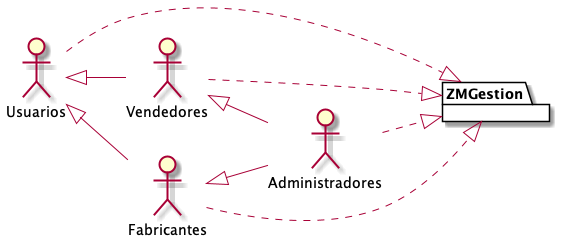
\includegraphics[width=\textwidth,height=0.40\textheight,keepaspectratio]{ModeladoDeCasosDeUso/DiagramaDeCasosDeUso/DiagramaContexto}
		\caption{Diagrama de contexto}
	\label{fig:DiagramaContexto}
	\end{figure}
	\subsection{Diagrama de subsistema}
	\begin{figure}[H]
		\centering
		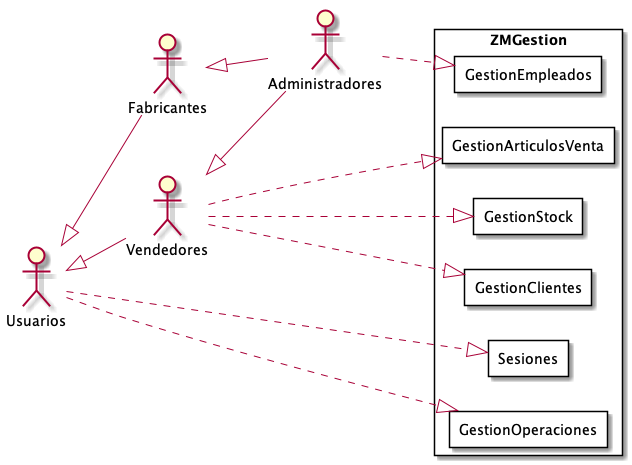
\includegraphics[width=\textwidth,height=0.90\textheight,keepaspectratio]{ModeladoDeCasosDeUso/DiagramaDeCasosDeUso/DiagramaSubsistema}
		\caption{Diagrama de subsistema }
	\label{fig:DiagramaSubsistema}
	\end{figure}
	\begin{figure}[H]
		\centering
		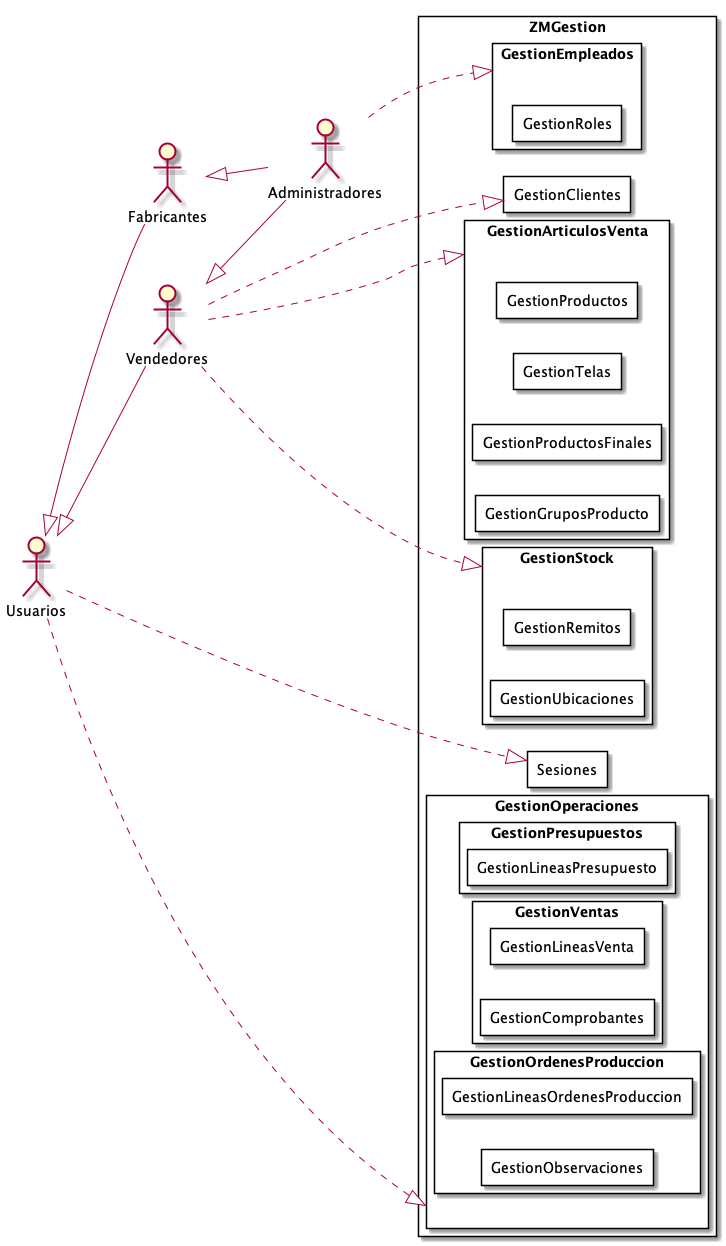
\includegraphics[width=\textwidth,height=0.90\textheight,keepaspectratio]{ModeladoDeCasosDeUso/DiagramaDeCasosDeUso/DiagramaSubsistemaDetallado}
		\caption{Diagrama de subsistema detallado}
	\label{fig:DiagramaSubsistemaDetallado}
	\end{figure}
	\clearpage %salto de pagina
	\subsection{Listado de casos de uso}
	\label{sec:listadoCasoUso}
	\begin{itemize}
		\item Sesiones
		\begin{itemize}
			\itemCaseUse{iniciarSesion}{Iniciar sesión}
			\itemCaseUse{cerrarSesion}{Cerrar sesión}
		\end{itemize}
		\item Gestión empleados
		\begin{itemize}
			\itemCaseUse{crearEmpleado}{Crear empleado}
			\itemCaseUse{buscarAvanzadoEmpleados}{Buscar avanzado empleados}
			\itemCaseUse{darBajaEmpleado}{Dar de baja empleado}
			\itemCaseUse{darAltaEmpleado}{Dar de alta empleado}
			\itemCaseUse{modificarEmpleado}{Modificar empleado}
			\itemCaseUse{borrarEmpleado}{Borrar empleado}
		\end{itemize}
		\item Gestión roles
		\begin{itemize}
			\itemCaseUse{crearRol}{Crear rol}
			\itemCaseUse{listarRoles}{Listar roles}
			\itemCaseUse{modificarRol}{Modificar rol}
			\itemCaseUse{borrarRol}{Borrar rol}
		\end{itemize}
		\item Gestión productos
		\begin{itemize}
			\itemCaseUse{crearProducto}{Crear producto}
			\itemCaseUse{buscarAvanzadoProductos}{Buscar avanzado productos}
			\itemCaseUse{darBajaProducto}{Dar de baja producto}
			\itemCaseUse{darAltaProducto}{Dar de alta producto}
			\itemCaseUse{modificarProducto}{Modificar producto}
			\itemCaseUse{borrarProducto}{Borrar producto}
		\end{itemize}
		\item Gestión telas
		\begin{itemize}
			\itemCaseUse{crearTela}{Crear tela}
			\itemCaseUse{listarTelas}{Listar telas}
			\itemCaseUse{darBajaTela}{Dar de baja tela}
			\itemCaseUse{darAltaTela}{Dar de alta tela}
			\itemCaseUse{modificarTela}{Modificar tela}
			\itemCaseUse{borrarTela}{Borrar tela}
		\end{itemize}
		\item Gestión productos finales
		\begin{itemize}
			\itemCaseUse{crearProductoFinal}{Crear producto final}
			\itemCaseUse{buscarAvanzadoProductosFinales}{Buscar avanzado productos finales}
			\itemCaseUse{darBajaProductoFinal}{Dar de baja producto final}
			\itemCaseUse{darAltaProductoFinal}{Dar de alta producto final}
			\itemCaseUse{modificarProductoFinal}{Modificar producto final}
			\itemCaseUse{borrarProductoFinal}{Borrar producto final}
		\end{itemize}
		\item Gestión grupos de producto
		\begin{itemize}
			\itemCaseUse{crearGrupoProducto}{Crear grupo de producto}
			\itemCaseUse{listarGruposProducto}{Listar grupos de producto}
			\itemCaseUse{darBajaGrupoProducto}{Dar de baja grupo de producto}
			\itemCaseUse{darAltaGrupoProducto}{Dar de alta grupo de producto}
			\itemCaseUse{modificarGrupoProducto}{Modificar grupo de producto}
			\itemCaseUse{borrarGrupoProducto}{Borrar grupo de producto}
			\itemCaseUse{listarProductosGrupo}{Listar productos por grupo}
			\itemCaseUse{modificarPreciosGrupo}{Modificar precios de producto por grupo}
		\end{itemize}
		\item Gestión ubicaciones
		\begin{itemize}
			\itemCaseUse{crearUbicacion}{Crear ubicación}
			\itemCaseUse{listarUbicaciones}{Listar ubicaciones}
			\itemCaseUse{darBajaUbicacion}{Dar de baja ubicación}
			\itemCaseUse{darAltaUbicacion}{Dar de alta ubicación}
			\itemCaseUse{modificarUbicacion}{Modificar ubicación}
			\itemCaseUse{borrarUbicacion}{Borrar ubicación}
		\end{itemize}
		\item Gestión remitos
		\begin{itemize}
			\itemCaseUse{crearRemito}{Crear remito}
			\itemCaseUse{buscarAvanzadoRemitos}{Buscar avanzado remitos}
			\itemCaseUse{cancelarRemito}{Cancelar remito}
			\itemCaseUse{descancelarRemito}{Descancelar remito}
			\itemCaseUse{entregarRemito}{Entregar remito}
			\itemCaseUse{borrarRemito}{Borrar remito}
			\itemCaseUse{listarLineasRemito}{Listar líneas de remito}
		\end{itemize}
		\item Gestión líneas de remito
		\begin{itemize}
			\itemCaseUse{crearLineaRemito}{Crear línea remito}
			\itemCaseUse{modificarLineaRemito}{Modificar línea de remito}
			\itemCaseUse{borrarLineaRemito}{Borrar línea de remito}
		\end{itemize}
		\item Gestión clientes
		\begin{itemize}
			\itemCaseUse{crearCliente}{Crear cliente}
			\itemCaseUse{buscarAvanzadoClientes}{Buscar avanzado clientes}
			\itemCaseUse{darBajaCliente}{Dar de baja cliente}
			\itemCaseUse{darAltaCliente}{Dar de alta cliente}
			\itemCaseUse{modificarCliente}{Modificar cliente}
			\itemCaseUse{borrarCliente}{Borrar cliente}
			\itemCaseUse{listarDomicilios}{Listar domicilios}
		\end{itemize}
		\item Gestión domicilios
		\begin{itemize}
			\itemCaseUse{crearDomicilio}{Crear domicilio}
			\itemCaseUse{borrarDomicilio}{Borrar domicilio}
		\end{itemize}
		\item Gestión presupuestos
		\begin{itemize}
			\itemCaseUse{crearPresupuesto}{Crear presupuesto}
			\itemCaseUse{buscarAvanzadoPresupuestos}{Buscar avanzado presupuestos}
			\itemCaseUse{modificarPresupuesto}{Modificar presupuesto}
			\itemCaseUse{borrarPresupuesto}{Borrar presupuesto}
			\itemCaseUse{transformarPresupuestosEnVenta}{Transformar presupuesto en venta}
			\itemCaseUse{generarPresupuestoPDF}{Generar presupuesto en formato PDF}
			\itemCaseUse{enviarPresupuestoEmail}{Enviar presupuesto por correo electrónico}
			\itemCaseUse{listarLineasPresupuesto}{Listar líneas de presupuesto}
		\end{itemize}
		\item Gestión líneas de presupuesto
		\begin{itemize}
			\itemCaseUse{crearLineaPresupuesto}{Crear línea de presupuesto}
			\itemCaseUse{modificarLineaPresupuesto}{Modificar línea de presupuesto}
			\itemCaseUse{borrarLineaPresupuesto}{Borrar línea de presupuesto}
		\end{itemize}
		\item Gestión ventas
		\begin{itemize}
			\itemCaseUse{crearVenta}{Crear venta}
			\itemCaseUse{buscarAvanzadoVentas}{Buscar avanzado ventas}
			\itemCaseUse{listarLineasVenta}{Listar líneas de venta}
			\itemCaseUse{modificarVenta}{Modificar venta}
			\itemCaseUse{borrarVenta}{Borrar venta}
			\itemCaseUse{generarOrdenProduccionDesdeVenta}{Generar orden de producción a partir de venta}
			\itemCaseUse{generarRemitoDesdeVenta}{Generar remito a partir de venta}
			\itemCaseUse{crearComprobante}{Crear comprobante} 
			\itemCaseUse{revisarVenta}{Revisar venta}
		\end{itemize}
		\item Gestión líneas de venta
		\begin{itemize}
			\itemCaseUse{crearLineaVenta}{Crear línea de venta}
			\itemCaseUse{modificarLineaVenta}{Modificar línea de venta}
			\itemCaseUse{borrarLineaVenta}{Borrar línea de venta}
			\itemCaseUse{cancelarLineaVenta}{Cancelar línea de venta}
		\end{itemize}
		\item Gestión comprobantes
		\begin{itemize}
			\itemCaseUse{buscarAvanzadoComprobantes}{Buscar avanzado comprobantes}
			\itemCaseUse{modificarComprobante}{Modificar comprobante}
			\itemCaseUse{borrarComprobante}{Borrar comprobante}
		\end{itemize}
		\item Gestión órdenes de producción
		\begin{itemize}
			\itemCaseUse{crearOrdenProduccion}{Crear orden de producción}
			\itemCaseUse{buscarAvanzadoOrdenesProduccion}{Buscar avanzado órdenes de producción}
			\itemCaseUse{modificarOrdenProduccion}{Modificar orden de producción}
			\itemCaseUse{listarLineasOrdenProduccion}{Listar líneas de orden de producción}
			\itemCaseUse{borrarOrdenProduccion}{Borrar orden de producción}
			\itemCaseUse{cancelarOrdenProduccion}{Cancelar orden de producción}
			\itemCaseUse{listarTareasLineaOrdenProduccion}{Listar tareas de línea de orden de producción}
		\end{itemize}
		\item Gestión líneas de órdenes de producción
		\begin{itemize}
			\itemCaseUse{crearLineaOrdenProduccion}{Crear línea de orden de producción}
			\itemCaseUse{modificarLineaOrdenProduccion}{Modificar línea de orden de producción}
			\itemCaseUse{borrarLineaOrdenProduccion}{Borrar línea de orden de producción}
			\itemCaseUse{verificarLineaOrdenProduccion}{Verificar línea de orden de producción}
			\itemCaseUse{cancelarLineaOrdenProduccion}{Cancelar línea de orden de producción}	
			\itemCaseUse{reanudarLineaOrdenProduccion}{Reanudar línea de orden de producción}		
		\end{itemize}
		\clearpage
		\item Gestión observaciones
		\begin{itemize}
			\itemCaseUse{crearObservacion}{Crear observación}
			\itemCaseUse{listarObservaciones}{Listar observaciones}
			\itemCaseUse{borrarObservacion}{Borrar observación}
		\end{itemize}
		\item Gestión tareas
		\begin{itemize}
			\itemCaseUse{crearTarea}{Crear tarea}
			\itemCaseUse{borrarTarea}{Borrar tarea}
			\itemCaseUse{finalizarTarea}{Finalizar tarea}
			\itemCaseUse{verificarTarea}{Verificar tarea}
			\itemCaseUse{pausarTarea}{Pausar tarea}
			\itemCaseUse{reanudarTarea}{Reanudar tarea}
			\itemCaseUse{cancelarTarea}{Cancelar tarea}
			\itemCaseUse{ejecutarTarea}{Ejecutar tarea}
		\end{itemize}
	\end{itemize}	
	\subsection{Diagrama de casos de uso}
	\begin{figure}[H]
		\centering
		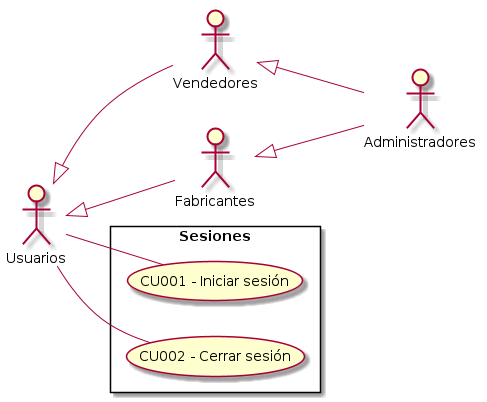
\includegraphics[width=\textwidth,height=0.30\textheight,keepaspectratio]{ModeladoDeCasosDeUso/DiagramaDeCasosDeUso/Sesiones}
		\caption{Diagrama de casos de uso para sesiones}
	\label{fig:Sesiones}
	\end{figure}
	\begin{figure}[H]
		\centering
		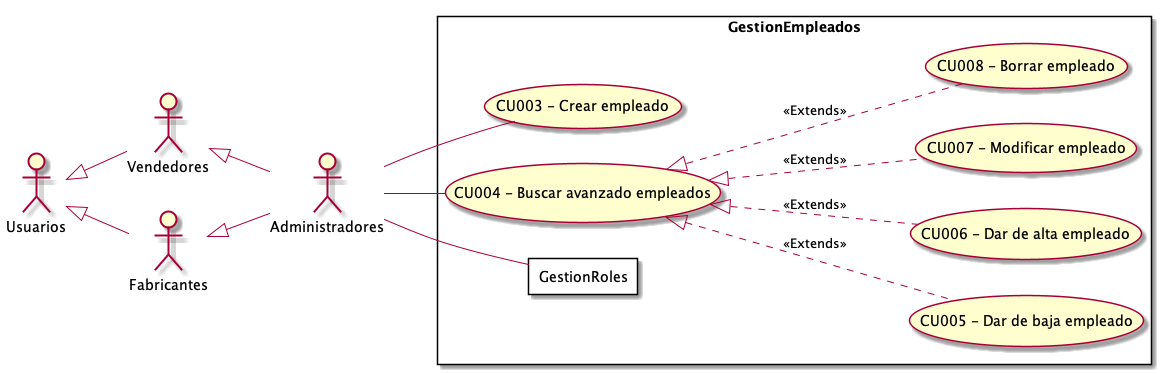
\includegraphics[width=\textwidth,height=0.40\textheight,keepaspectratio]{ModeladoDeCasosDeUso/DiagramaDeCasosDeUso/GestionEmpleados}
		\caption{Diagrama de casos de uso para la gestión de empleados}
	\label{fig:GestionEmpleados}
	\end{figure}
	\begin{figure}[H]
		\centering
		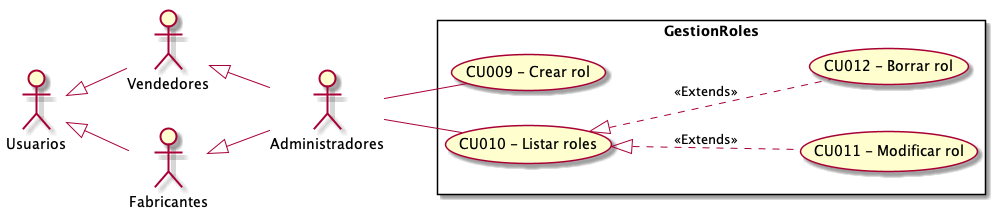
\includegraphics[width=\textwidth,height=0.90\textheight,keepaspectratio]{ModeladoDeCasosDeUso/DiagramaDeCasosDeUso/GestionRoles}
		\caption{Diagrama de casos de uso para la gestión de roles}
	\label{fig:GestionRoles}
	\end{figure}
	\begin{figure}[H]
		\centering
		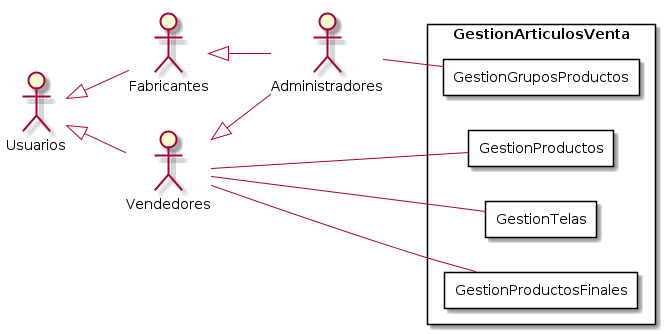
\includegraphics[width=\textwidth,height=0.90\textheight,keepaspectratio]{ModeladoDeCasosDeUso/DiagramaDeCasosDeUso/GestionArticulosVenta}
		\caption{Diagrama de casos de uso para la gestión de artículos de venta}
	\label{fig:GestionArticulosVenta}
	\end{figure}
    \begin{figure}[H]
		\centering
		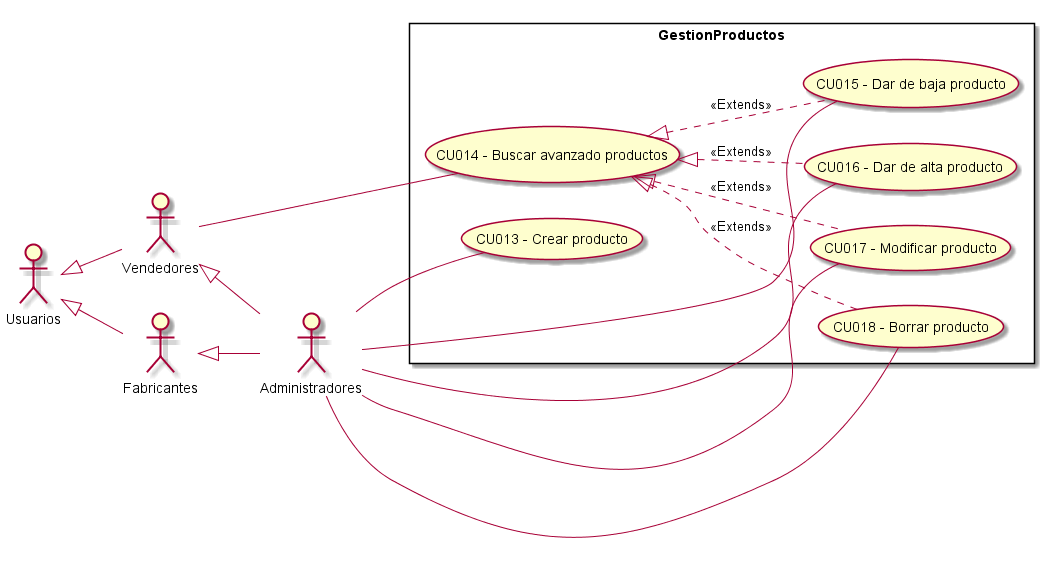
\includegraphics[width=\textwidth,height=0.90\textheight,keepaspectratio]{ModeladoDeCasosDeUso/DiagramaDeCasosDeUso/GestionProductos}
		\caption{Diagrama de casos de uso para la gestión de productos}
	\label{fig:GestionProductos}
    \end{figure}
    \begin{figure}[H]
		\centering
		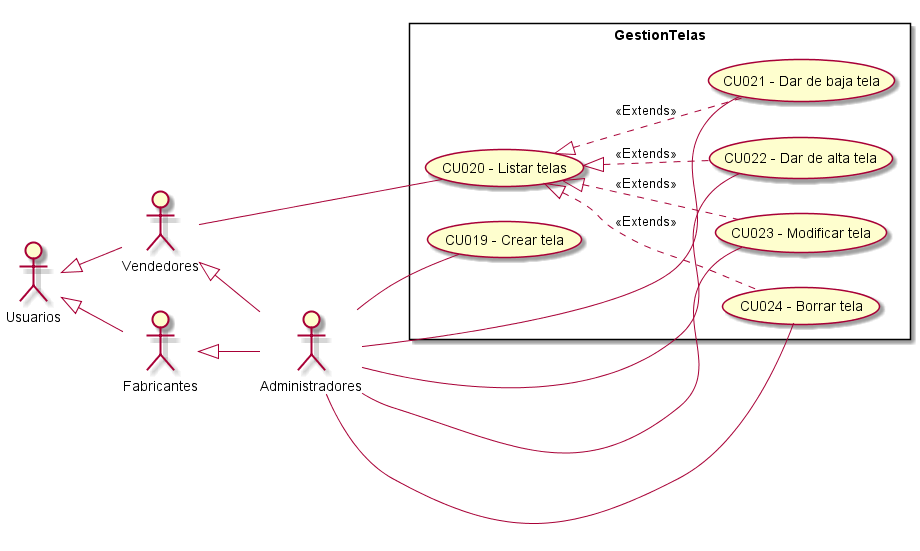
\includegraphics[width=\textwidth,height=0.90\textheight,keepaspectratio]{ModeladoDeCasosDeUso/DiagramaDeCasosDeUso/GestionTelas}
		\caption{Diagrama de casos de uso para la gestión de telas}
	\label{fig:GestionTelas}
    \end{figure}
    \begin{figure}[H]
		\centering
		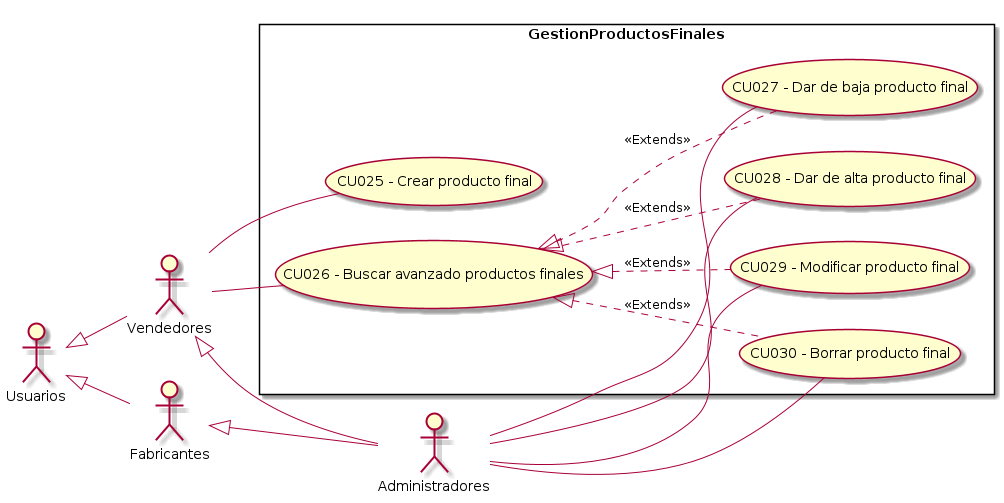
\includegraphics[width=\textwidth,height=0.90\textheight,keepaspectratio]{ModeladoDeCasosDeUso/DiagramaDeCasosDeUso/GestionProductosFinales}
		\caption{Diagrama de casos de uso para la gestión de productos finales}
	\label{fig:GestionProductosFinales}
    \end{figure}
    \begin{figure}[H]
		\centering
		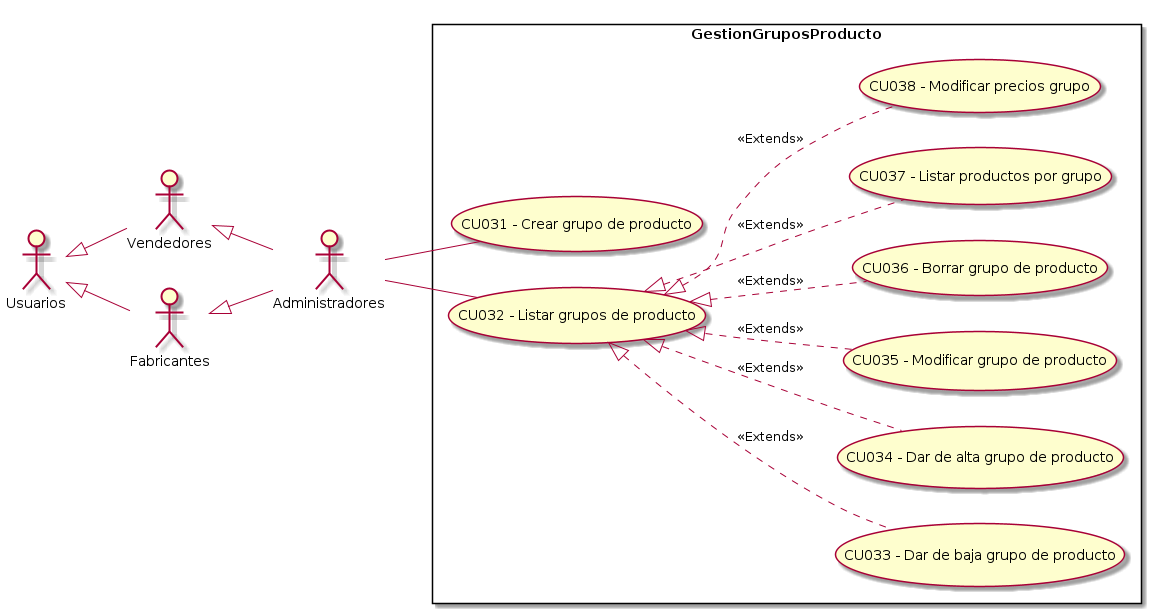
\includegraphics[width=\textwidth,height=0.90\textheight,keepaspectratio]{ModeladoDeCasosDeUso/DiagramaDeCasosDeUso/GestionGruposProducto}
		\caption{Diagrama de casos de uso para la gestión de grupos de producto}
	\label{fig:GestionGruposProducto}
	\end{figure}
	\begin{figure}[H]
		\centering
		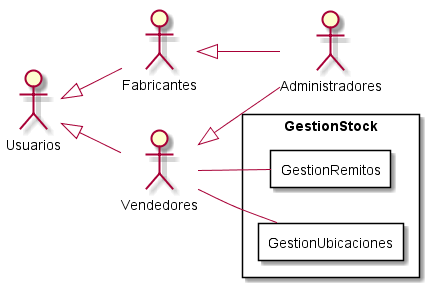
\includegraphics[width=\textwidth,height=0.90\textheight,keepaspectratio]{ModeladoDeCasosDeUso/DiagramaDeCasosDeUso/GestionStock}
		\caption{Diagrama de casos de uso para la gestión de stock}
	\label{fig:GestionStock}
	\end{figure}
	\begin{figure}[H]
		\centering
		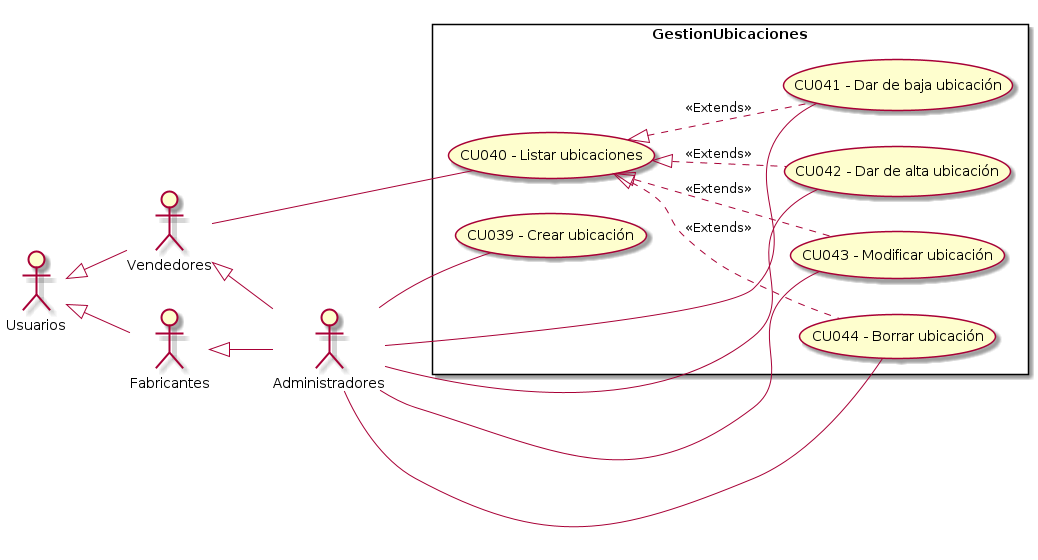
\includegraphics[width=\textwidth,height=0.90\textheight,keepaspectratio]{ModeladoDeCasosDeUso/DiagramaDeCasosDeUso/GestionUbicaciones}
		\caption{Diagrama de casos de uso para la gestión de ubicaciones}
	\label{fig:GestionUbicaciones}
    \end{figure}
	\begin{figure}[H]
		\centering
		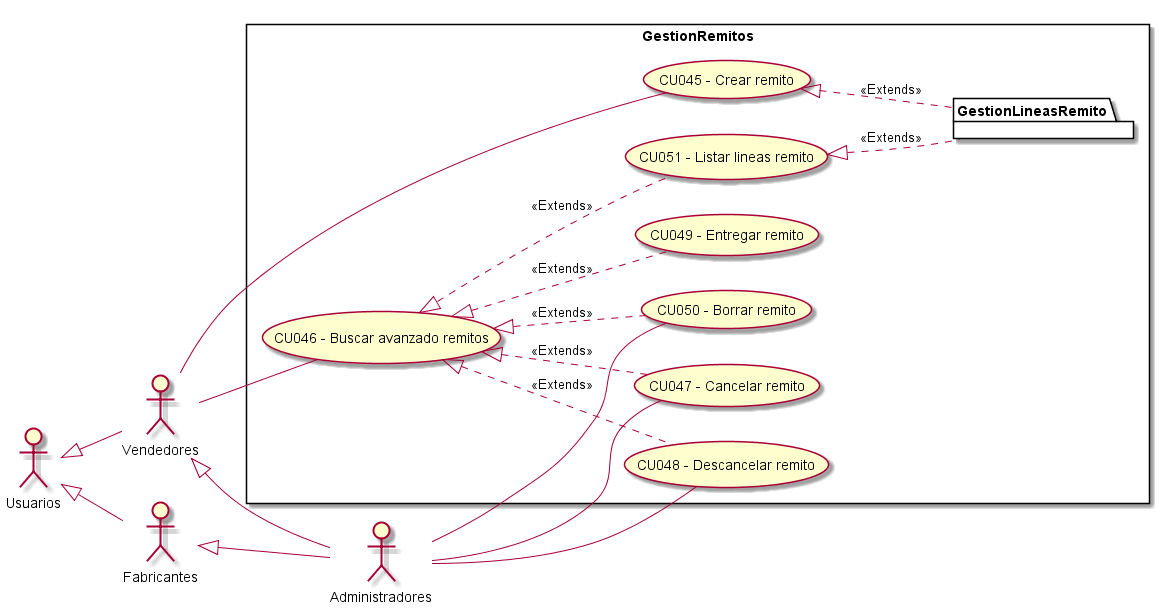
\includegraphics[width=\textwidth,height=0.90\textheight,keepaspectratio]{ModeladoDeCasosDeUso/DiagramaDeCasosDeUso/GestionRemitos}
		\caption{Diagrama de casos de uso para la gestión de remitos}
	\label{fig:GestionRemitos}
	\end{figure}
	\begin{figure}[H]
		\centering
		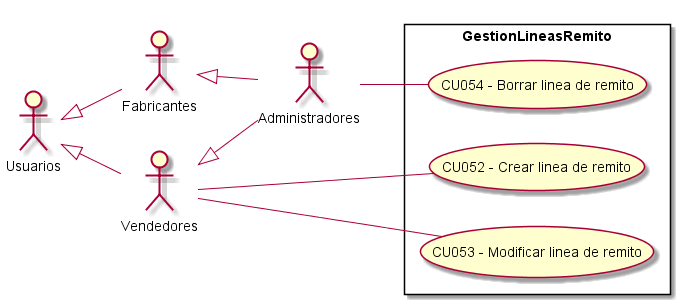
\includegraphics[width=\textwidth,height=0.90\textheight,keepaspectratio]{ModeladoDeCasosDeUso/DiagramaDeCasosDeUso/GestionLineasRemito}
		\caption{Diagrama de casos de uso para la gestión de líneas de remito}
	\label{fig:GestionLineasRemito}
    \end{figure}
    \begin{figure}[H]
		\centering
		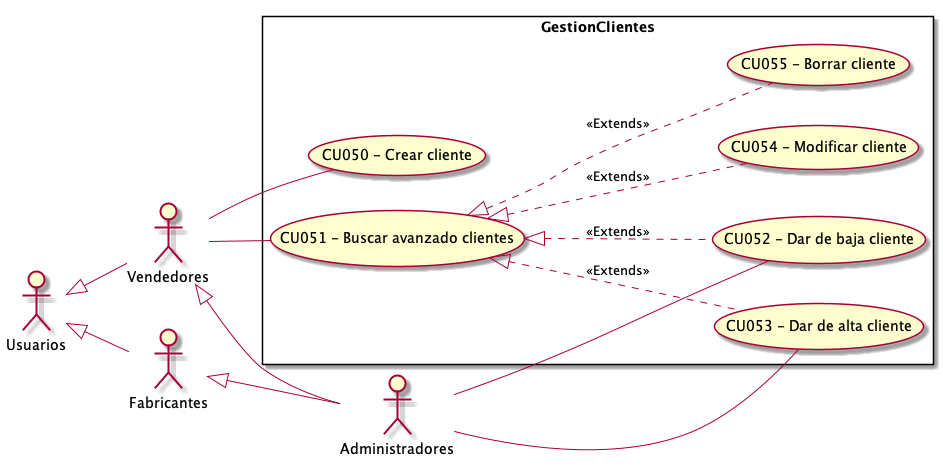
\includegraphics[width=\textwidth,height=0.90\textheight,keepaspectratio]{ModeladoDeCasosDeUso/DiagramaDeCasosDeUso/GestionClientes}
		\caption{Diagrama de casos de uso para la gestión de clientes}
	\label{fig:GestionClientes}
	\end{figure}
	\begin{figure}[H]
		\centering
		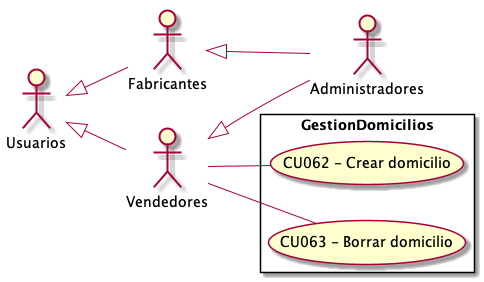
\includegraphics[width=\textwidth,height=0.90\textheight,keepaspectratio]{ModeladoDeCasosDeUso/DiagramaDeCasosDeUso/GestionDomicilios}
		\caption{Diagrama de casos de uso para la gestión de domicilios}
	\label{fig:GestionDomicilios}
	\end{figure}
	\begin{figure}[H]
		\centering
		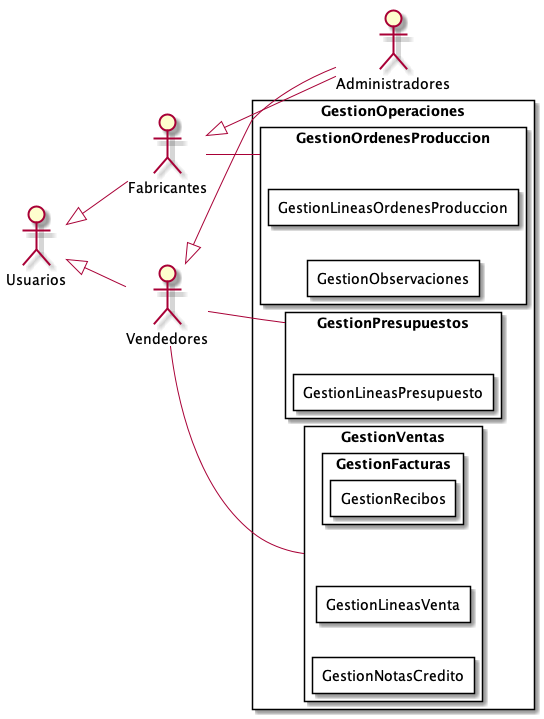
\includegraphics[width=\textwidth,height=0.90\textheight,keepaspectratio]{ModeladoDeCasosDeUso/DiagramaDeCasosDeUso/GestionOperaciones}
		\caption{Diagrama de casos de uso para la gestión de operaciones}
	\label{fig:GestionOperaciones}
	\end{figure}
    \begin{figure}[H]
		\centering
		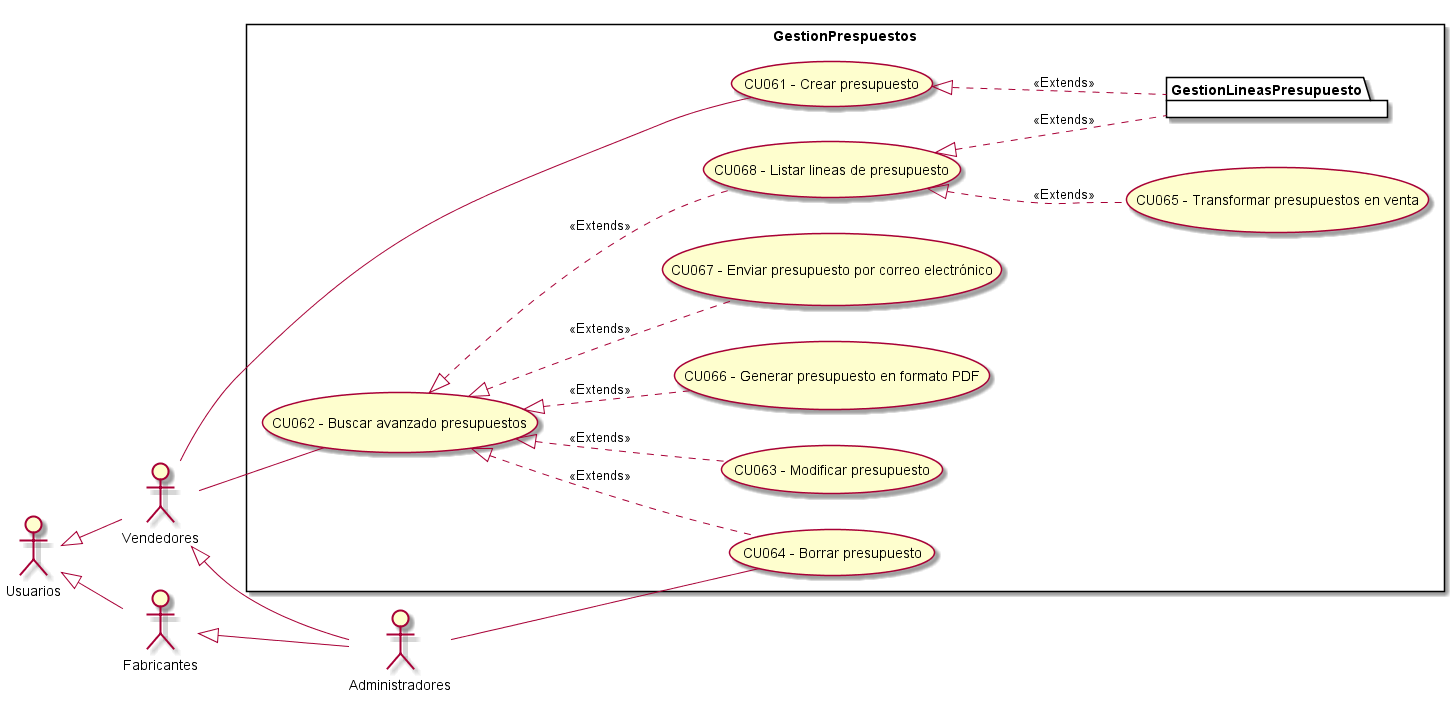
\includegraphics[width=\textwidth,height=0.90\textheight,keepaspectratio]{ModeladoDeCasosDeUso/DiagramaDeCasosDeUso/GestionPresupuestos}
		\caption{Diagrama de casos de uso para la gestión de presupuestos}
	\label{fig:GestionPresupuestos}
    \end{figure}
    \begin{figure}[H]
		\centering
		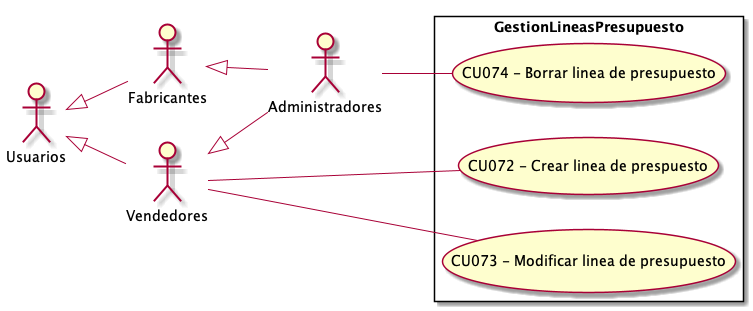
\includegraphics[width=\textwidth,height=0.90\textheight,keepaspectratio]{ModeladoDeCasosDeUso/DiagramaDeCasosDeUso/GestionLineasPresupuesto}
		\caption{Diagrama de casos de uso para la gestión de líneas de presupuesto}
	\label{fig:GestionLineasPresupuesto}
    \end{figure}
    \begin{figure}[H]
		\centering
		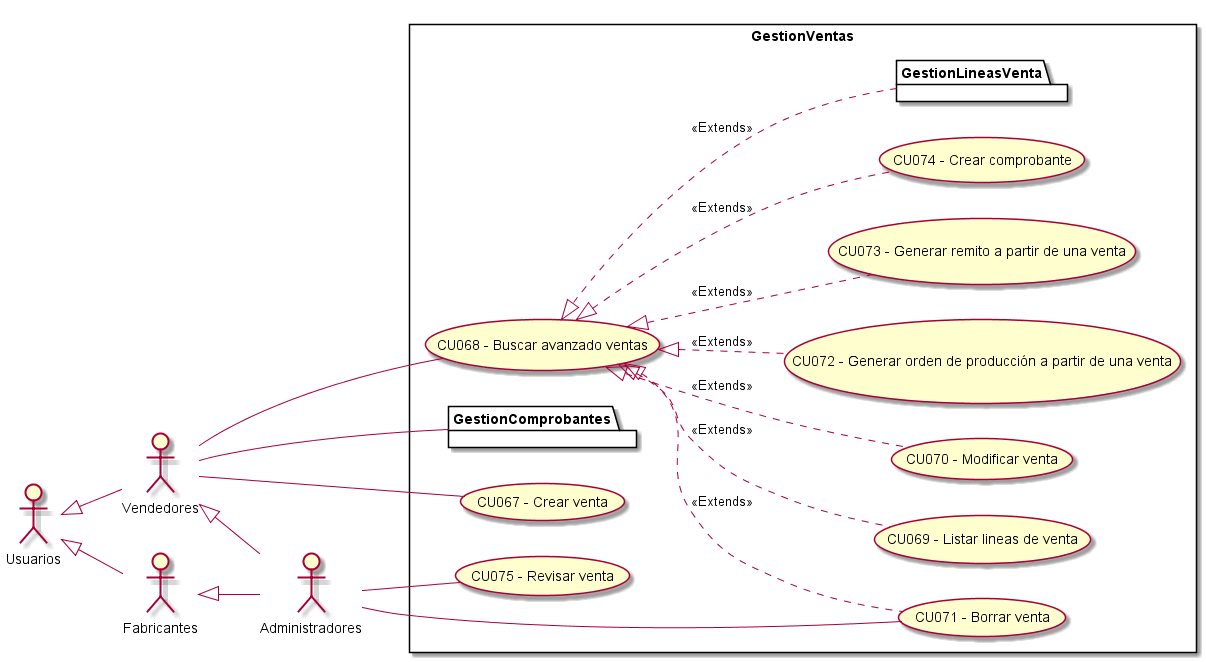
\includegraphics[width=\textwidth,height=0.90\textheight,keepaspectratio]{ModeladoDeCasosDeUso/DiagramaDeCasosDeUso/GestionVentas}
		\caption{Diagrama de casos de uso para la gestión de ventas}
	\label{fig:GestionVentas}
    \end{figure}
    \begin{figure}[H]
		\centering
		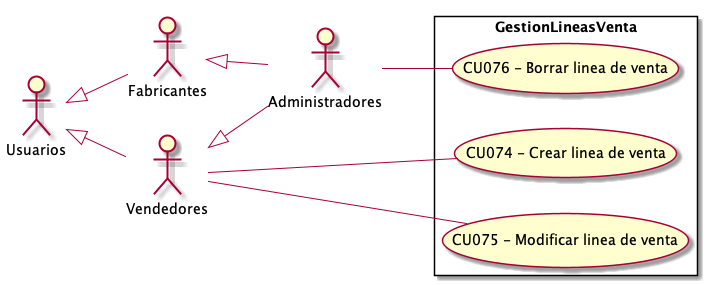
\includegraphics[width=\textwidth,height=0.90\textheight,keepaspectratio]{ModeladoDeCasosDeUso/DiagramaDeCasosDeUso/GestionLineasVenta}
		\caption{Diagrama de casos de uso para la gestión de líneas de venta}
	\label{fig:GestionLineasVenta}
    \end{figure}
    \begin{figure}[H]
		\centering
		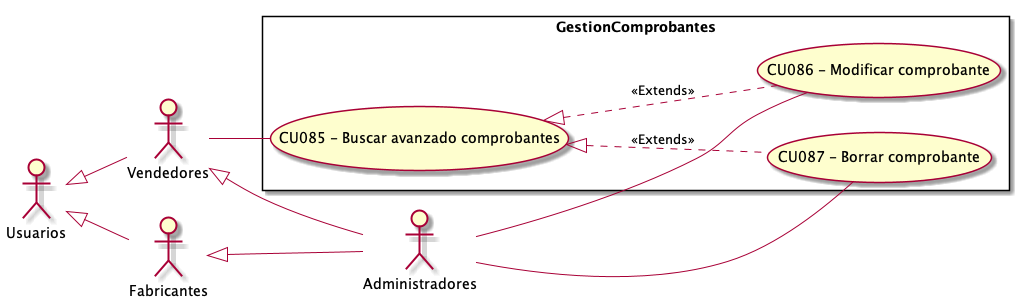
\includegraphics[width=\textwidth,height=0.90\textheight,keepaspectratio]{ModeladoDeCasosDeUso/DiagramaDeCasosDeUso/GestionComprobantes}
		\caption{Diagrama de casos de uso para la gestión de comprobantes}
	\label{fig:GestionComprobantes}
    \end{figure}
    \begin{figure}[H]
		\centering
		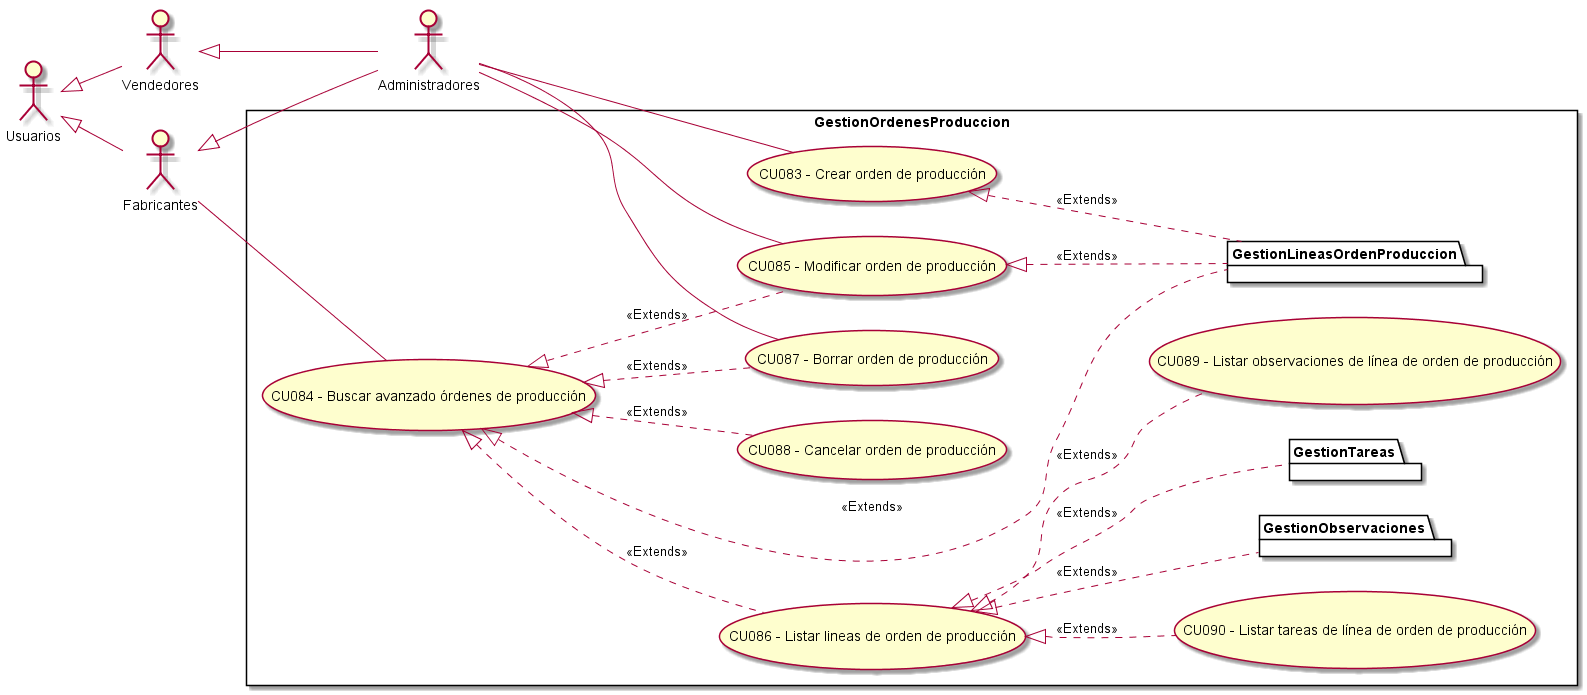
\includegraphics[width=\textwidth,height=0.90\textheight,keepaspectratio]{ModeladoDeCasosDeUso/DiagramaDeCasosDeUso/GestionOrdenesProduccion}
		\caption{Diagrama de casos de uso para la gestión de órdenes de producción}
	\label{fig:GestionOrdenesProduccion}
    \end{figure}
    \begin{figure}[H]
		\centering
		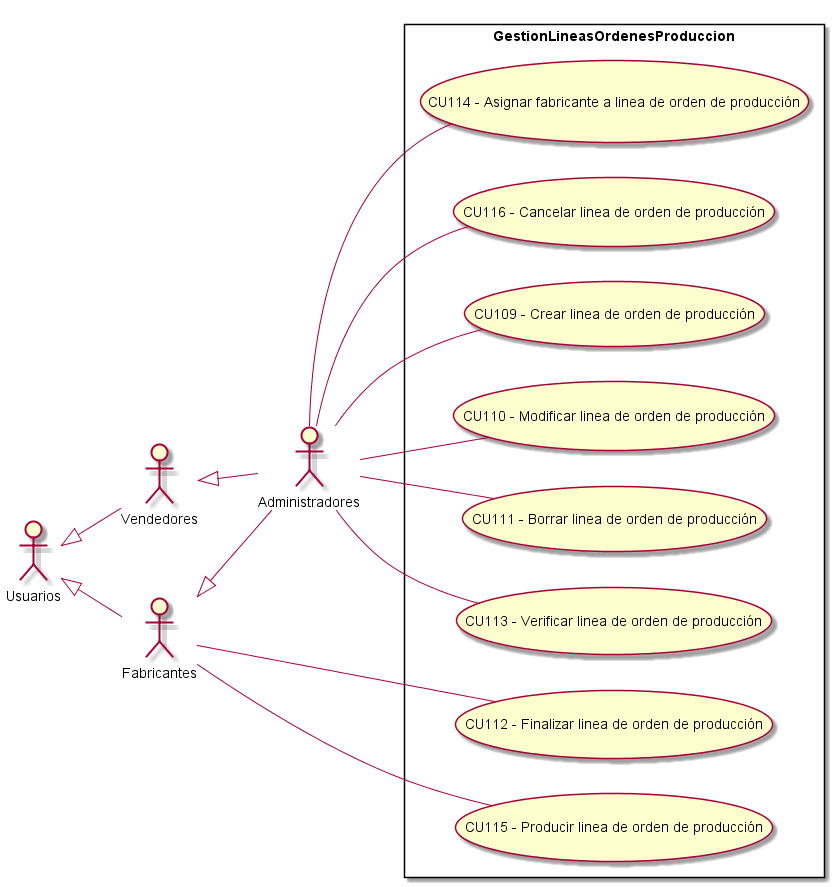
\includegraphics[width=\textwidth,height=0.90\textheight,keepaspectratio]{ModeladoDeCasosDeUso/DiagramaDeCasosDeUso/GestionLineasOrdenesProduccion}
		\caption{Diagrama de casos de uso para la gestión de líneas de órdenes de producción}
	\label{fig:GestionLineasOrdenesProduccion}
    \end{figure}
    \begin{figure}[H]
		\centering
		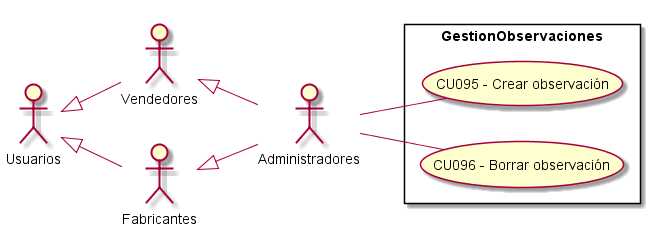
\includegraphics[width=\textwidth,height=0.90\textheight,keepaspectratio]{ModeladoDeCasosDeUso/DiagramaDeCasosDeUso/GestionObservaciones}
		\caption{Diagrama de casos de uso para la gestión de observaciones}
	\label{fig:GestionObservaciones}
	\end{figure}
	\begin{figure}[H]
		\centering
		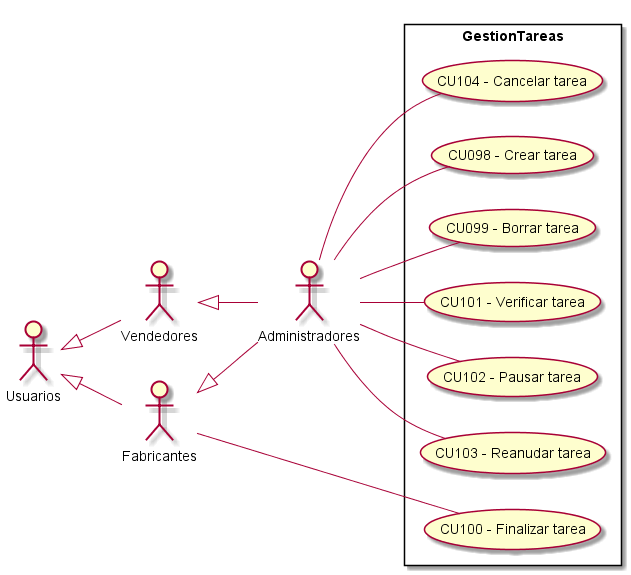
\includegraphics[width=\textwidth,height=0.90\textheight,keepaspectratio]{ModeladoDeCasosDeUso/DiagramaDeCasosDeUso/GestionTareas}
		\caption{Diagrama de casos de uso para la gestión de tareas}
	\label{fig:GestionTareas}
	\end{figure}
	\clearpage %salto de pagina
	\subsection{Descripción textual de los casos de uso y diagramas de actividad}
		A continuación se encuentran los casos de uso más relevantes del sistema. Los restantes pueden ser consultados en el Anexo.
		%GestionRemitos
		
\renewcommand{\caseUseShortName}{crearRemito} %cammelCase name

\renewcommand{\caseUseCreated}{05/03/2020} %Fecha creación
\renewcommand{\caseUseModified}{05/03/2020} %Fecha modificación
\renewcommand{\caseUseName}{\CUcrearRemito - Crear remito } %{\CUcammelCase - Title}

\renewcommand{\caseUseSummary}{Este caso de uso permite a un vendedor de ZMGestion crear un remito.} %Resumen
\renewcommand{\caseUsePeople}{Vendedores: desea crear un remito.} %Actor: Meta
\renewcommand{\caseUsePreconditions}{
	\caseUseRow{Haber iniciado sesión en el sistema y tener el permiso necesario para realizar esta función.} %Precondiciones
}
\renewcommand{\caseUsePostconditions}{
	\caseUseRow{Ninguna.} %Postcondiciones
}
\renewcommand{\caseUseScene}{ %Escenario principal
    \addCaseUseStep{El vendedor accede a la pantalla para crear remitos.}
    \addCaseUseStep{ZMGestion muestra un formulario para que el vendedor seleccione el tipo de remito (Entrada o Salida), la ubicación, de entrada o salida según corresponda, y los productos cuestion. Indicando que todos los campos son obligatorios.}
    \addCaseUseStep{El vendedor completa los campos requeridos.} 
    \addCaseUseStep{ZMGestion crea el remito.}
}
\renewcommand{\alternativeCaseUse}{ %Flujos alternativos
	\newAlternative{A1: El vendedor ha dejado un campo obligatorio vacio.}{2} %Flujo alternativo A1.
	\caseUseRow{La secuencia A1 comienza luego del punto 2 del escenario principal.} %¡Indicar número paso!
    \alternativeRow{ZMGestion muestra un mensaje de error indicando que ha dejado un campo obligatorio vacio.}
    \caseUseRow{El escenario vuelve al punto 2.}
    \caseUseRow{}

}

\item Caso de uso \caseUseName
\input{Capitulos/Capitulo4/CasosUso/generalTable.tex}

%DIAGRAMA DE ACTIVIDAD
%\lineabreak[0]
%\activityDiagram{\caseUseShortName}{Diagrama de actividad - \caseUseName}
		
\renewcommand{\caseUseShortName}{} %cammelCase name

\renewcommand{\caseUseCreated}{15/02/2020} %Fecha creación
\renewcommand{\caseUseModified}{15/02/2020} %Fecha modificación
\renewcommand{\caseUseName}{\CU - } %{\CUcammelCase - Title}

\renewcommand{\caseUseSummary}{} %Resumen
\renewcommand{\caseUsePeople}{} %Actor: Meta
\renewcommand{\caseUsePreconditions}{
	\caseUseRow{Haber iniciado sesión en el sistema.} %Precondiciones
}
\renewcommand{\caseUsePostconditions}{
	\caseUseRow{Ninguna.} %Postcondiciones
}
\renewcommand{\caseUseScene}{ %Escenario principal
    \addCaseUseStep{}
    \addCaseUseStep{}
    \addCaseUseStep{}
    \addCaseUseStep{}
    \addCaseUseStep{}
    \addCaseUseStep{}
    \addCaseUseStep{}
    \addCaseUseStep{}
}
\renewcommand{\alternativeCaseUse}{ %Flujos alternativos
	\newAlternative{A1: Error al .}{NUMERO} %Flujo alternativo A1.
	\caseUseRow{La secuencia A1 comienza luego del punto NUMERO del escenario principal.} %¡Indicar número paso!
    \alternativeRow{}
    \alternativeRow{}
    \alternativeRow{}
    \alternativeRow{}
    \alternativeRow{}
    \alternativeRow{}
    
    \caseUseRow{}

	\newAlternative{A2: Error al .}{NUMERO} %Flujo alternativo A2.
    \caseUseRow{La secuencia A2 comienza luego del punto NUMERO del escenario principal.}%¡Indicar número paso!
    \alternativeRow{}
    \alternativeRow{}
    \alternativeRow{}
    \alternativeRow{}
    \alternativeRow{}
    \alternativeRow{}
}
\renewcommand{\caseUseRequirementsGUI}{
	\caseUseRow{Teclado, Mouse y Pantalla} %Requisitos interfaz de usuario
}
\renewcommand{\caseUseResponseTime}{La interfaz debe responder dentro de un tiempo máximo de 10 segundos.} %Requisitos funcionales: Tiempo de respuesta
\renewcommand{\caseUseConcurrence}{} %Requisitos funcionales: Concurrencia
\renewcommand{\caseUseAvailability}{} %Requisitos funcionales: Disponibilidad

\item Caso de uso \caseUseName
\input{Capitulos/Capitulo4/CasosUso/generalTable.tex}

%DIAGRAMA DE ACTIVIDAD
%\lineabreak[0]
%\activityDiagram{\caseUseShortName}{Diagrama de actividad - \caseUseName}
		\renewcommand{\caseUseShortName}{cancelarRemito} %cammelCase name

\renewcommand{\caseUseCreated}{11/03/2020} %Fecha creación
\renewcommand{\caseUseModified}{11/03/2020} %Fecha modificación
\renewcommand{\caseUseName}{\CUcancelarRemito\ - Cancelar remito} %{\CUcammelCase - Title}

\renewcommand{\caseUseSummary}{Este caso de uso permite a un administrador de ZMGestion cancelar un remito.} %Resumen
\renewcommand{\caseUsePeople}{Administradores: quiere cancelar un remito.} %Actor: Meta
\renewcommand{\caseUsePreconditions}{
    \caseUseRow{Haber ejecutado con éxito el \CUbuscarAvanzadoRemitos (Buscar avanzado remitos)} %Precondiciones
}
\renewcommand{\caseUsePostconditions}{
    \caseUseRow{Ninguna.} %Postcondiciones
}
\renewcommand{\caseUseScene}{ %Escenario principal
    \addCaseUseStep{El administrador indica el remito que desea cancelar.}
    \addCaseUseStep{ZMGestion pasa el estado del remito a `Cancelado'.}
}
\renewcommand{\alternativeCaseUse}{ %Flujos alternativos
    \newAlternative{A1: El remito se encuentra en un estado distinto de `Creado'.}{1} %Flujo alternativo A1.
    \caseUseRow{La secuencia A1 comienza luego del punto 1 del escenario principal.} %¡Indicar número paso!
    \alternativeRow{ZMGestion muestra un mensaje de error indicando que no se puede cancelar dicho remito.}
    \caseUseRow{El escenario vuelve al punto 1.}
    \caseUseRow{}
}


\item Caso de uso \caseUseName
\input{Capitulos/Capitulo4/CasosUso/generalTable.tex}

%DIAGRAMA DE ACTIVIDAD
%\lineabreak[0]
%\activityDiagram{\caseUseShortName}{Diagrama de actividad - \caseUseName}
		\renewcommand{\caseUseShortName}{descancelarRemito} %cammelCase name

\renewcommand{\caseUseCreated}{11/03/2020} %Fecha creación
\renewcommand{\caseUseModified}{11/03/2020} %Fecha modificación
\renewcommand{\caseUseName}{\CUdescancelarRemito\ - Descancelar remito} %{\CUcammelCase - Title}

\renewcommand{\caseUseSummary}{Este caso de uso permite a un administrador de ZMGestion descancelar un remito cancelado.} %Resumen
\renewcommand{\caseUsePeople}{Administradores: quiere descancelar un remito cancelado.} %Actor: Meta
\renewcommand{\caseUsePreconditions}{
    \caseUseRow{Haber ejecutado con éxito el \CUbuscarAvanzadoRemitos (Buscar avanzado remitos)} %Precondiciones
}
\renewcommand{\caseUsePostconditions}{
    \caseUseRow{Ninguna.} %Postcondiciones
}
\renewcommand{\caseUseScene}{ %Escenario principal
    \addCaseUseStep{El administrador indica el remito que desea descancelar.}
    \addCaseUseStep{ZMGestion pasa el estado del remito a `Creado'.}
}
\renewcommand{\alternativeCaseUse}{ %Flujos alternativos
    \newAlternative{A1: El remito se encuentra en un estado distinto de `Cancelado'.}{1} %Flujo alternativo A1.
    \caseUseRow{La secuencia A1 comienza luego del punto 1 del escenario principal.} %¡Indicar número paso!
    \alternativeRow{ZMGestion muestra un mensaje de error indicando que no se puede descancelar dicho remito.}
    \caseUseRow{El escenario vuelve al punto 1.}
    \caseUseRow{}
    \newAlternative{A2: El remito no posee lineas de remito.}{1}
    %Debido a que puede ocurrir que las lineas de venta (que representaban una linea de remito)
    %que tenian el idRemito que fue cancelado puede ser reemplazado por otro remito nuevo
    %y quedar sin lineas de remito el remito cancelado.
    \caseUseRow{La secuencia A1 comienza luego del punto 1 del escenario principal.} %¡Indicar número paso!
    \alternativeRow{ZMGestion muestra un mensaje de error indicando que el remito se encuentra vacío.}
    \caseUseRow{El escenario vuelve al punto 1.}
    \caseUseRow{}
}

\item Caso de uso \caseUseName
\input{Capitulos/Capitulo4/CasosUso/generalTable.tex}

%DIAGRAMA DE ACTIVIDAD
		\renewcommand{\caseUseShortName}{entregarRemito} %cammelCase name

\renewcommand{\caseUseCreated}{11/03/2020} %Fecha creación
\renewcommand{\caseUseModified}{11/03/2020} %Fecha modificación
\renewcommand{\caseUseName}{\CUentregarRemito\ - Entregar remito} %{\CUcammelCase - Title}

\renewcommand{\caseUseSummary}{Este caso de uso permite a un administrador de ZMGestion marcar como entregado todos los productos de un remito.} %Resumen
\renewcommand{\caseUsePeople}{Administradores: quiere indicar que todos los productos de un remito fueron entregado y ademas especificar la fecha.} %Actor: Meta
\renewcommand{\caseUsePreconditions}{
    \caseUseRow{Haber ejecutado con éxito el \CUbuscarAvanzadoRemitos (Buscar avanzado remitos)} %Precondiciones
}
\renewcommand{\caseUsePostconditions}{
    \caseUseRow{Ninguna.} %Postcondiciones
}
\renewcommand{\caseUseScene}{ %Escenario principal
    \addCaseUseStep{El administrador indica el remito que desea asignarle una fecha de entrega.}
    \addCaseUseStep{ZMGestion muestra un formulario para que el administrador indique la fecha en que todos los productos del remito fueron entregados.}
    \addCaseUseStep{El administrador selecciona la fecha en que los productos fueron entregados.}
    \addCaseUseStep{ZMGestion pasa el estado del remito a `Entregado' y a cada línea de remito la pasa al estado de `Entregada'.}
}
\renewcommand{\alternativeCaseUse}{ %Flujos alternativos
    \newAlternative{A1: El remito seleccionado se encuentra en un estado `Creado'.}{1} %Flujo alternativo A1.
    \caseUseRow{La secuencia A1 comienza luego del punto 1 del escenario principal.} %¡Indicar número paso!
    \alternativeRow{ZMGestion muestra un mensaje de error indicando que no se puede marcar como entregado los productos de dicho remito.}
    \caseUseRow{El escenario vuelve al punto 1.}
    \caseUseRow{}

    \newAlternative{A2: La fecha ingresada por el administrador es anterior a la fecha de creación del remito.}{3} %Flujo alternativo A1.
    \caseUseRow{La secuencia A2 comienza luego del punto 3 del escenario principal.} %¡Indicar número paso!
    \alternativeRow{ZMGestion muestra un mensaje de error indicando que la fecha de entrega de los productos no puede ser anterior a la fecha de creación del remito.}
    \caseUseRow{El escenario vuelve al punto 1.}
    \caseUseRow{}

}

%\item Caso de uso \caseUseName
\input{Capitulos/Capitulo4/CasosUso/generalTable.tex}

%DIAGRAMA DE ACTIVIDAD
%\lineabreak[0]
%\activityDiagram{\caseUseShortName}{Diagrama de actividad - \caseUseName}
		
\renewcommand{\caseUseShortName}{} %cammelCase name

\renewcommand{\caseUseCreated}{15/02/2020} %Fecha creación
\renewcommand{\caseUseModified}{15/02/2020} %Fecha modificación
\renewcommand{\caseUseName}{\CU - } %{\CUcammelCase - Title}

\renewcommand{\caseUseSummary}{} %Resumen
\renewcommand{\caseUsePeople}{} %Actor: Meta
\renewcommand{\caseUsePreconditions}{
	\caseUseRow{Haber iniciado sesión en el sistema.} %Precondiciones
}
\renewcommand{\caseUsePostconditions}{
	\caseUseRow{Ninguna.} %Postcondiciones
}
\renewcommand{\caseUseScene}{ %Escenario principal
    \addCaseUseStep{}
    \addCaseUseStep{}
    \addCaseUseStep{}
    \addCaseUseStep{}
    \addCaseUseStep{}
    \addCaseUseStep{}
    \addCaseUseStep{}
    \addCaseUseStep{}
}
\renewcommand{\alternativeCaseUse}{ %Flujos alternativos
	\newAlternative{A1: Error al .}{NUMERO} %Flujo alternativo A1.
	\caseUseRow{La secuencia A1 comienza luego del punto NUMERO del escenario principal.} %¡Indicar número paso!
    \alternativeRow{}
    \alternativeRow{}
    \alternativeRow{}
    \alternativeRow{}
    \alternativeRow{}
    \alternativeRow{}
    
    \caseUseRow{}

	\newAlternative{A2: Error al .}{NUMERO} %Flujo alternativo A2.
    \caseUseRow{La secuencia A2 comienza luego del punto NUMERO del escenario principal.}%¡Indicar número paso!
    \alternativeRow{}
    \alternativeRow{}
    \alternativeRow{}
    \alternativeRow{}
    \alternativeRow{}
    \alternativeRow{}
}
\renewcommand{\caseUseRequirementsGUI}{
	\caseUseRow{Teclado, Mouse y Pantalla} %Requisitos interfaz de usuario
}
\renewcommand{\caseUseResponseTime}{La interfaz debe responder dentro de un tiempo máximo de 10 segundos.} %Requisitos funcionales: Tiempo de respuesta
\renewcommand{\caseUseConcurrence}{} %Requisitos funcionales: Concurrencia
\renewcommand{\caseUseAvailability}{} %Requisitos funcionales: Disponibilidad

\item Caso de uso \caseUseName
\input{Capitulos/Capitulo4/CasosUso/generalTable.tex}

%DIAGRAMA DE ACTIVIDAD
%\lineabreak[0]
%\activityDiagram{\caseUseShortName}{Diagrama de actividad - \caseUseName}
		
\renewcommand{\caseUseShortName}{listarLineasRemito} %cammelCase name

\renewcommand{\caseUseCreated}{11/03/2020} %Fecha creación
\renewcommand{\caseUseModified}{11/03/2020} %Fecha modificación
\renewcommand{\caseUseName}{\CUlistarLineasRemito - Listar líneas de remito} %{\CUcammelCase - Title}

\renewcommand{\caseUseSummary}{Este caso de uso permite a un vendedor de ZMGestion listar las líneas de remito de un remito determinado.} %Resumen
\renewcommand{\caseUsePeople}{Vendedores: quiere listar las líneas de remito de un remito existente.} %Actor: Meta
\renewcommand{\caseUsePreconditions}{
	\caseUseRow{Haber realizado con éxito el \CUbuscarAvanzadoRemitos\ (Buscar avanzado remitos).} %Precondiciones
}
\renewcommand{\caseUsePostconditions}{
	\caseUseRow{Ninguna.} %Postcondiciones
}
\renewcommand{\caseUseScene}{ %Escenario principal
    \addCaseUseStep{El vendedor indica el remito del cual desea listar sus líneas de remito.}
    \addCaseUseStep{ZMGestion lista las líneas de remito existentes del remito seleccionado.}
}
\renewcommand{\alternativeCaseUse}{ %Flujos alternativos
	\newAlternative{A1: El remito no posee líneas de remito.}{1} %Flujo alternativo A1.
	\caseUseRow{La secuencia A1 comienza luego del punto 1 del escenario principal.} %¡Indicar número paso!
    \alternativeRow{ZMGestion muestra un mensaje de error indicando que el remito seleccionado no posee ninguna linea de remito.}
    \caseUseRow{El escenario vuelve al punto 1.}
    \caseUseRow{}
}
%\item Caso de uso \caseUseName
\input{Capitulos/Capitulo4/CasosUso/generalTable.tex}

%DIAGRAMA DE ACTIVIDAD
%\lineabreak[0]
%\activityDiagram{\caseUseShortName}{Diagrama de actividad - \caseUseName}

		%GestionLineasRemito
		\renewcommand{\caseUseShortName}{crearLineaRemito} %cammelCase name

\renewcommand{\caseUseCreated}{10/03/2020} %Fecha creación
\renewcommand{\caseUseModified}{10/03/2020} %Fecha modificación
\renewcommand{\caseUseName}{\CUcrearLineaRemito\ - Crear linea de remito.} %{\CUcammelCase - Title}

\renewcommand{\caseUseSummary}{Este caso de uso permite a un vendedor de ZMGestion crear una linea de remito para un determinado remito.} %Resumen
\renewcommand{\caseUsePeople}{Vendedores: quiere crear una linea de remito.} %Actor: Meta
\renewcommand{\caseUsePreconditions}{
	\caseUseRow{Estar ejecutando el \CUcrearRemito (Crear remito).} %Precondiciones
}
\renewcommand{\caseUsePostconditions}{
	\caseUseRow{Ningúna.} %Postcondiciones
}
\renewcommand{\caseUseScene}{ %Escenario principal
    \addCaseUseStep{El vendedor desea agregar una linea de remito a un determinado remito.}
    \addCaseUseStep{ZMGestion muestra un formulario para que el vendedor seleccione un producto, tela, lustre, indique la cantidad del mismo y la ubicación (de entrada o salida según corresponda). Indicando que el producto y la cantidad son obligatorios.}
    \addCaseUseStep{El vendedor selecciona producto, tela, lustre, la cantidad que desea producir y la ubicación.}
    \addCaseUseStep{ZMGestion crea la linea de remito en estado `Pendiente de entrega' y la asocia al remito correspondiente.}
}
\renewcommand{\alternativeCaseUse}{ %Flujos alternativos
    \newAlternative{A1: La cantidad indicada es menor o igual a cero.}{3} %Flujo alternativo A1.
    \caseUseRow{La secuencia A1 comienza luego del punto 3 del escenario principal.} %¡Indicar número paso!
    \alternativeRow{ZMGestion muestra un mensaje de error indicando que debe ingresar una cantidad mayor a cero.}
    \caseUseRow{El escenario vuelve al punto 2.}
    \caseUseRow{}
    \newAlternative{A2: El producto, tela, lustre y ubicación indicado ya se encuentra en el remito.}{3} %Flujo alternativo A2.
    \caseUseRow{La secuencia A2 comienza luego del punto 3 del escenario principal.} %¡Indicar número paso!
    \alternativeRow{ZMGestion muestra un mensaje de error indicando que la combinación de producto, tela y lustre ya se encuentra en el remito.}
    \caseUseRow{El escenario vuelve al punto 2.}
    \caseUseRow{}
    \newAlternative{A3: El vendedor ha dejado un campo obligatorio vacio.}{3} %Flujo alternativo A2.
    \caseUseRow{La secuencia A3 comienza luego del punto 3 del escenario principal.}%¡Indicar número paso!
    \alternativeRow{ZMGestion muestra un mensaje de error indicando que dicho campo es requerido.}
    \caseUseRow{El escenario vuelve al punto 2.}
    \caseUseRow{}
}

\item Caso de uso \caseUseName
\input{Capitulos/Capitulo4/CasosUso/generalTable.tex}

%DIAGRAMA DE ACTIVIDAD
%\lineabreak[0]
%\activityDiagram{\caseUseShortName}{Diagrama de actividad - \caseUseName}
		
\renewcommand{\caseUseShortName}{modificarLineaRemito} %cammelCase name

\renewcommand{\caseUseCreated}{10/03/2020} %Fecha creación
\renewcommand{\caseUseModified}{10/03/2020} %Fecha modificación
\renewcommand{\caseUseName}{\CUmodificarLineaRemito - Modificar línea remito} %{\CUcammelCase - Title}

\renewcommand{\caseUseSummary}{Este caso de uso permite a un vendedor de ZMGestion modificar una línea de remito.} %Resumen
\renewcommand{\caseUsePeople}{Vendedores: desea modificar una línea deremito.} %Actor: Meta
\renewcommand{\caseUsePreconditions}{
	\caseUseRow{Haber ejecutado con éxito el \CUlistarLineasRemito (Listar lineas de remito).} %Precondiciones
}
\renewcommand{\caseUsePostconditions}{
	\caseUseRow{Ninguna.} %Postcondiciones
}
\renewcommand{\caseUseScene}{ %Escenario principal
    \addCaseUseStep{El administrador indica la línea de remito que desea modificar.}
    \addCaseUseStep{ZMGestion muestra un formulario autocompletado con los datos de la linea de remito seleccionada, producto, tela, lustre, cantidady ubicación. Indicando que todos los el producto y la cantidad son obligatorios.}
    \addCaseUseStep{El administrador modifica el producto, tela, lustre, cantidad y ubicación.}
    \addCaseUseStep{ZMGestion modifica la línea de remito y muestra un mensaje indicando el éxito de la operación.}

}
\renewcommand{\alternativeCaseUse}{ %Flujos alternativos
	\newAlternative{A1: La línea de remito seleccionada no se encuentra en estado de `Pendiente de entrega'.}{1} %Flujo alternativo A1.
	\caseUseRow{La secuencia A1 comienza luego del punto 1 del escenario principal.} %¡Indicar número paso!
    \alternativeRow{ZMgestion muestra un mensaje de error indicando que la línea de remito no puede modificarse.}
    \caseUseRow{El escenario vuelve al punto 1.}
    \caseUseRow{}

	\newAlternative{A2: La cantidad es menor o igual que cero.}{3} %Flujo alternativo A2.
    \caseUseRow{La secuencia A2 comienza luego del punto 3 del escenario principal.}%¡Indicar número paso!
    \alternativeRow{ZMGestion muestra un mensaje de error indicando que la cantidad debe ser mayor que cero.}
    \caseUseRow{El escenario vuelve al punto 2.}
    \caseUseRow{}

    \newAlternative{A3: La combinación de producto, tela, lustre y ubicación
    ya se encuentra en el remito.}{3} %Flujo alternativo A2.
    \caseUseRow{La secuencia A3 comienza luego del punto 3 del escenario principal.}%¡Indicar número paso!
    \alternativeRow{ZMGestion muestra un mensaje de error indicando que ya existe una línea de remito identica en el remito.}
    \caseUseRow{El escenario vuelve al punto 2.}
    \caseUseRow{}

    \newAlternative{A4: El vendedor ha dejado un campo obligatorio vacío.}{3} %Flujo alternativo A2.
    \caseUseRow{La secuencia A4 comienza luego del punto 3 del escenario principal.}%¡Indicar número paso!
    \alternativeRow{ZMGestion muestra un mensaje de error indicando que dicho campo es requerido.}
    \caseUseRow{El escenario vuelve al punto 2.}
    \caseUseRow{}
}

\item Caso de uso \caseUseName
\input{Capitulos/Capitulo4/CasosUso/generalTable.tex}

%DIAGRAMA DE ACTIVIDAD
%\lineabreak[0]
%\activityDiagram{\caseUseShortName}{Diagrama de actividad - \caseUseName}
		\renewcommand{\caseUseShortName}{borrarLineaRemito} %cammelCase name

\renewcommand{\caseUseCreated}{10/03/2020} %Fecha creación
\renewcommand{\caseUseModified}{10/03/2020} %Fecha modificación
\renewcommand{\caseUseName}{\CUborrarLineaRemito\ - Borrar linea de remito.} %{\CUcammelCase - Title}

\renewcommand{\caseUseSummary}{Este caso de uso permite a un administrador de ZMGestion borrar una linea de remito de un remito determinad.} %Resumen
\renewcommand{\caseUsePeople}{Administradores: quiere borrar una linea de remito.} %Actor: Meta
\renewcommand{\caseUsePreconditions}{
	\caseUseRow{Haber ejecutado con éxito el \CUlistarLineasRemito (Listar lineas de remito).} %Precondiciones
}
\renewcommand{\caseUsePostconditions}{
	\caseUseRow{Ninguna.} %Postcondiciones
}
\renewcommand{\caseUseScene}{ %Escenario principal
    \addCaseUseStep{El vendedor indica la linea de remito que desea borrar.}
    \addCaseUseStep{ZMGestion borra la linea de remito.}
}
\renewcommand{\alternativeCaseUse}{ %Flujos alternativos

    %VER QUE A1 TAMBIEN SE PUEDE HACER REVISANDO SI LA LINEA ESTA UTILIZADA O NO

	\newAlternative{A1: La linea seleccionada tiene un estado distinto de `Pendiente de entrega'.}{1} %Flujo alternativo A1.
	\caseUseRow{La secuencia A1 comienza luego del punto 1 del escenario principal.} %¡Indicar número paso!
    \alternativeRow{ZMGestion muestra un mensaje de error indicando que no se puede borrar la linea de remito.}
    \caseUseRow{El escenario vuelve al punto 1.}
}

%\item Caso de uso \caseUseName
\input{Capitulos/Capitulo4/CasosUso/generalTable.tex}

%DIAGRAMA DE ACTIVIDAD
%\lineabreak[0]
%\activityDiagram{\caseUseShortName}{Diagrama de actividad - \caseUseName}

		%GestionPresupuestos
		
\renewcommand{\caseUseShortName}{transformarPresupuestosEnVenta} %cammelCase name

\renewcommand{\caseUseCreated}{04/02/2020} %Fecha creación
\renewcommand{\caseUseModified}{04/02/2020} %Fecha modificación
\renewcommand{\caseUseName}{\CUtransformarPresupuestosEnVenta\ - Transformar presupuestos en venta.} %{\CUcammelCase - Title}

\renewcommand{\caseUseSummary}{Este caso de uso permite a un vendedor transformar uno o más presupuestos existentes en venta.} %Resumen
\renewcommand{\caseUsePeople}{Vendedores: quiere realizar una venta a partir de uno o más presupuestos.} %Actor: Meta
\renewcommand{\caseUsePreconditions}{
	\caseUseRow{Haber realizado con éxito el CU65 (Buscar avanzado presupuestos).} %Precondiciones
}
\renewcommand{\caseUsePostconditions}{
	\caseUseRow{Ninguna.} %Postcondiciones
}
\renewcommand{\caseUseScene}{ %Escenario principal
    \addCaseUseStep{El vendedor indica uno o más presupuestos a partir de los cuales desea generar la venta.}
    \addCaseUseStep{ZMGestion muestra un formulario para que el vendedor seleccione un cliente existente y se ejecuta el CU71 (Listar líneas de presupuesto) para cada presupuesto seleccionado, mostrando una opción por cada linea para indicar si desea añadirla a la venta.}
    \addCaseUseStep{El vendedor selecciona un cliente existente y las líneas de presupuestos que desea agregar a la venta.}
    \addCaseUseStep{ZMGestion crea una venta en estado "En creación" para el cliente seleccionado, ejecuta el \CUcrearLineaVenta\ (Crear linea de venta) con los valores de producto, cantidad y precio de cada linea de presupuesto seleccionada.}
    \addCaseUseStep{Si el vendedor desea modificar alguna de las líneas de venta agregadas ejecuta el \CUmodificarLineaVenta\ (Modificar linea de venta). Si el vendedor desea quitar alguna linea de venta agregada se ejecuta el \CUborrarLineaVenta\ (Borrar linea de venta). Si el vendedor desea agregar una nueva linea de venta se ejecuta el \CUcrearLineaVenta\ (Crear linea de venta).}
    \addCaseUseStep{ZMGestión verifica que las líneas de ventas creadas tengan el precio actual del producto, en caso de que una o más líneas de venta tengan un precio distinto al precio actual, la venta se pasa al estado "En revisión", caso contrario se pasa al estado "Pendiente" y, en este caso, las líneas de presupuesto que se utilizaron para la venta se pasan al estado "Utilizadas" y las que no se utilizaron al estado "No utilizadas".}
}
\renewcommand{\alternativeCaseUse}{ %Flujos alternativos
	\newAlternative{A1: Uno o más de los presupuestos seleccionados se encuentra en estado "Vendido".}{1} %Flujo alternativo A1.
	\caseUseRow{La secuencia A1 comienza luego del punto 1 del escenario principal.} %¡Indicar número paso!
    \alternativeRow{ZMGestion muestra un mensaje de error indicando que uno de los presupuestos seleccionados se encuentra en estado "Vendido".}
    \caseUseRow{}
    \caseUseRow{El escenario vuelve al punto 1.}
    \newAlternative{A2:El vendedor ha dejado el campo de cliente vacío.}{3} %Flujo alternativo A2.
	\caseUseRow{La secuencia A2 comienza luego del punto 3 del escenario principal.} %¡Indicar número paso!
    \alternativeRow{ZMGestion muestra un mensaje de error indicando que debe seleccionar un cliente válido.}
    \caseUseRow{}
    \caseUseRow{El escenario vuelve al punto 2.}
    \newAlternative{A3:No se ingresó ninguna linea de venta.}{5} %Flujo alternativo A3.
	\caseUseRow{La secuencia A3 comienza luego del punto 5 del escenario principal.} %¡Indicar número paso!
    \alternativeRow{ZMGestion muestra un mensaje de error indicando que debe ingresar al menos una linea.}
    \caseUseRow{}
    \caseUseRow{El escenario vuelve al punto 5.}

}
%\item Caso de uso \caseUseName
\input{Capitulos/Capitulo4/CasosUso/generalTable.tex}

%DIAGRAMA DE ACTIVIDAD
%\lineabreak[0]
\activityDiagram{\caseUseShortName}{Diagrama de actividad - \caseUseName}

		%GestionVentas
		\renewcommand{\caseUseShortName}{crearVenta} %cammelCase name

\renewcommand{\caseUseCreated}{08/02/2020} %Fecha creación
\renewcommand{\caseUseModified}{08/02/2020} %Fecha modificación
\renewcommand{\caseUseName}{\CUcrearVenta - Crear venta} %{\CUcammelCase - Title}

\renewcommand{\caseUseSummary}{Este caso de uso permite a un vendedor de ZMGestion crear una venta para un cliente existente.} %Resumen
\renewcommand{\caseUsePeople}{Vendedores: quiere crear una venta para un cliente existente.} %Actor: Meta
\renewcommand{\caseUsePreconditions}{
	\caseUseRow{Haber iniciado sesión en el sistemay tener el permiso necesario para realizar esta función.} %Precondiciones
}
\renewcommand{\caseUsePostconditions}{
	\caseUseRow{Ninguna.} %Postcondiciones
}
\renewcommand{\caseUseScene}{ %Escenario principal
    \addCaseUseStep{El vendedor accede a la pantalla para crear ventas.}
    \addCaseUseStep{ZMGestion le muestra un formulario para que el vendedor seleccione un cliente.}
    \addCaseUseStep{El vendedor selecciona un cliente.}%3
    \addCaseUseStep{ZMGestion crea una venta en estado de "En revisión" para el cliente seleccionado.}%4
    \addCaseUseStep{ZMGestion pregunta si desea agregar una nueva linea de venta.}%5
    \addCaseUseStep{En caso afirmativo se ejecuta el \CUcrearLineaVenta (Crear linea de venta) y se vuelve a realizar la pregunta. En caso contrario ZMGestión verifica que las lineas de ventas creadas tengan el precio actual del producto, en caso de que todas las lineas de venta tengan el precio actual para el producto y tela seleccionados, la venta se pasa al estado "En edición", el estado de las lineas de presupuesto que se utilizaron se pasan a "Utilizadas" y las que no se utilizaron al estado "No utilizadas".} %REVISAR ESTADO DE LAS LINEAS DE VENTA. SIGUEN EN EDICION... SE DEBERIA CAMBIAR A ALGUN OTRO ESTADO? EL ESTADO DE LA VENTA SE DETERMINA A PARTIR DEL ESTADO DE LAS LINEAS DE VENTA Y CREAR UNA VENTA NO SIGNIFICA QUE HAYA HECHO UN PAGO...
    \addCaseUseStep{ZMGestión muestra un mensaje indicando el éxito de la operacion y vuelve al punto 5 del escenario principal.}
}
\renewcommand{\alternativeCaseUse}{ %Flujos alternativos
	\newAlternative{A1: No ha seleccionado ningún cliente.}{3} %Flujo alternativo A1.
	\caseUseRow{La secuencia A1 comienza luego del punto 3 del escenario principal.} %¡Indicar número paso!
    \alternativeRow{ZMGestion muestra un mensaje de error indicando que debe seleccionar un cliente.}
    \caseUseRow{El escenario vuelve al punto 2.}
    \caseUseRow{}
	\newAlternative{A2: No ha agregado ninguna linea de venta.}{6} %Flujo alternativo A2.
    \caseUseRow{La secuencia A2 comienza luego del punto 6 del escenario principal.}%¡Indicar número paso!
    \alternativeRow{ZMGestion muestra un mensaje de error indicando que debe agregar al menos una linea de venta.}
    \caseUseRow{El escenario vuelve al punto 5.}
    \caseUseRow{}
}

\item Caso de uso \caseUseName
\input{Capitulos/Capitulo4/CasosUso/generalTable.tex}

%DIAGRAMA DE ACTIVIDAD
%\lineabreak[0]
%\activityDiagram{AD_\caseUseShortName}{Diagrama de actividad - \caseUseName}
		
\renewcommand{\caseUseShortName}{listarLineasVenta} %cammelCase name

\renewcommand{\caseUseCreated}{13/02/2020} %Fecha creación
\renewcommand{\caseUseModified}{13/02/2020} %Fecha modificación
\renewcommand{\caseUseName}{\CUlistarLineasVenta - Listar líneas de venta} %{\CUcammelCase - Title}

\renewcommand{\caseUseSummary}{Este caso de uso permite a un vendedor de ZMGestion listar las líneas de venta de una venta determinada.} %Resumen
\renewcommand{\caseUsePeople}{Vendedores: quiere listar las líneas de venta de una venta existente.} %Actor: Meta
\renewcommand{\caseUsePreconditions}{
	\caseUseRow{Haber realizado con éxito el \CUbuscarAvanzadoVentas\ (Buscar avanzado ventas).} %Precondiciones
}
\renewcommand{\caseUsePostconditions}{
	\caseUseRow{Ninguna.} %Postcondiciones
}
\renewcommand{\caseUseScene}{ %Escenario principal
    \addCaseUseStep{El vendedor indica la venta a la cual desea listar sus líneas de venta.}
    \addCaseUseStep{ZMGestion lista las líneas de venta existentes de la venta seleccionada.}
}
\renewcommand{\alternativeCaseUse}{ %Flujos alternativos
	\newAlternative{A1: La venta no posee líneas de venta.}{1} %Flujo alternativo A1.
	\caseUseRow{La secuencia A1 comienza luego del punto 1 del escenario principal.} %¡Indicar número paso!
    \alternativeRow{ZMGestion muestra un mensaje indicando que la venta seleccionada no posee ninguna linea de venta.}
    \caseUseRow{El escenario vuelve al punto 1.}
    \caseUseRow{}
}
%\item Caso de uso \caseUseName
\input{Capitulos/Capitulo4/CasosUso/generalTable.tex}

%DIAGRAMA DE ACTIVIDAD
%\lineabreak[0]
%\activityDiagram{\caseUseShortName}{Diagrama de actividad - \caseUseName}
		
\renewcommand{\caseUseShortName}{generarOrdenProduccionDesdeVenta} %cammelCase name

\renewcommand{\caseUseCreated}{15/02/2020} %Fecha creación
\renewcommand{\caseUseModified}{15/02/2020} %Fecha modificación
\renewcommand{\caseUseName}{\CUgenerarOrdenProduccionDesdeVenta - Generar orden de producción a partir de venta} %{\CUcammelCase - Title}

\renewcommand{\caseUseSummary}{Este caso de uso permite a un administrador de ZMGestion crear una orden de producción a partir de una venta existente.} %Resumen
\renewcommand{\caseUsePeople}{Administradores: quiere crear una orden de producción a partir de una venta.} %Actor: Meta
\renewcommand{\caseUsePreconditions}{
	\caseUseRow{Haber ejecutado con éxito el \CUbuscarAvanzadoVentas (Buscar avanzado ventas).} %Precondiciones
}
\renewcommand{\caseUsePostconditions}{
	\caseUseRow{Ninguna.} %Postcondiciones
}
\renewcommand{\caseUseScene}{ %Escenario principal
    \addCaseUseStep{El administrador selecciona una venta a partir de la cual desea generar la orden de producción.}
    \addCaseUseStep{ZMGestion ejecuta el \CUlistarLineasVenta\ (Listar líneas de venta) para la venta seleccionada, mostrando una opción por cada línea para indicar si desea añadirla a la orden de producción.}
    \addCaseUseStep{El administrador selecciona las líneas de ventas que desea agregar a la orden de producción.}
    \addCaseUseStep{ZMGestion crea una orden de producción en estado "En creación" y ejecuta el \CUcrearLineaOrdenProduccion\ (Crear línea de orden de producción) con los valores de producto, tela, lustre y cantidad de la línea de venta seleccionada.}
    \addCaseUseStep{Si el administrador desea modificar alguna de las líneas de orden de producción agregadas ejecuta el \CUmodificarLineaOrdenProduccion\ (Modificar línea de orden de producción). Si el administrador desea quitar alguna línea de orden de producción agregada se ejecuta el \CUborrarLineaOrdenProduccion\ (Borrar línea de orden de producción). Si el administrador desea agregar una nueva línea de orden de producción se ejecuta el \CUcrearLineaOrdenProduccion\ (Crear línea de orden de producción).}
    \addCaseUseStep{ZMGestión pasa el estado de la orden de producción a `Pendiente'.}
}
\renewcommand{\alternativeCaseUse}{ %Flujos alternativos
	\newAlternative{A1: No se agregó ninguna línea de orden de producción.}{5} %Flujo alternativo A1.
	\caseUseRow{La secuencia A1 comienza luego del punto 5 del escenario principal.} %¡Indicar número paso!
    \alternativeRow{ZMGestion muestra un mensaje de error indicando que debe ingresar al menos una linea de orden de producción.}
    \caseUseRow{El escenario vuelve al punto 5.}
    \caseUseRow{}
}

\item Caso de uso \caseUseName
\input{Capitulos/Capitulo4/CasosUso/generalTable.tex}

%DIAGRAMA DE ACTIVIDAD
%\lineabreak[0]
%\activityDiagram{\caseUseShortName}{Diagrama de actividad - \caseUseName}
		
\renewcommand{\caseUseShortName}{generarRemitoDesdeVenta} %cammelCase name

\renewcommand{\caseUseCreated}{08/03/2020} %Fecha creación
\renewcommand{\caseUseModified}{08/03/2020} %Fecha modificación
\renewcommand{\caseUseName}{\CUgenerarRemitoDesdeVenta - Generar remito a partir de venta} %{\CUcammelCase - Title}

\renewcommand{\caseUseSummary}{Este caso de uso permite a un administrador de ZMGestion crear un remito a partir de una venta existente.} %Resumen
\renewcommand{\caseUsePeople}{Administradores: quiere crear un remito a partir de una venta.} %Actor: Meta
\renewcommand{\caseUsePreconditions}{
	\caseUseRow{Haber ejecutado con éxito el CU78 (Buscar avanzado ventas).} %Precondiciones
}
\renewcommand{\caseUsePostconditions}{
	\caseUseRow{Ninguna.} %Postcondiciones
}
\renewcommand{\caseUseScene}{ %Escenario principal
    \addCaseUseStep{El administrador selecciona una venta a partir de la cual desea generar el remito.}
    \addCaseUseStep{ZMGestion ejecuta el \CUlistarLineasVenta\ (Listar líneas de venta) para la venta seleccionada, mostrando una opción por cada línea para indicar si desea añadirla a el remito.}
    \addCaseUseStep{El administrador selecciona las líneas de ventas que desea agregar a el remito.}
    \addCaseUseStep{ZMGestion crea un remito en estado `En creación' y ejecuta el \CUcrearLineaRemito\ (Crear línea de remito) con los valores de producto, tela, lustre y cantidad de la línea de venta seleccionada.}
    \addCaseUseStep{Si el administrador desea quitar alguna línea de remito agregada se ejecuta el \CUborrarLineaRemito\ (Borrar línea de remito).}
    \addCaseUseStep{ZMGestión pasa el estado de el remito a `Creado'.}
}
\renewcommand{\alternativeCaseUse}{ %Flujos alternativos
	\newAlternative{A1: No se agregó ninguna línea de remito.}{3} %Flujo alternativo A1.
	\caseUseRow{La secuencia A1 comienza luego del punto 3 del escenario principal.} %¡Indicar número paso!
    \alternativeRow{ZMGestion muestra un mensaje de error indicando que debe ingresar al menos una linea de remito.}
    \caseUseRow{El escenario vuelve al punto 2.}
    \caseUseRow{}
    \newAlternative{A2: El total pagado no es suficiente para realizar el remito.}{3} %Flujo alternativo A1.
	\caseUseRow{La secuencia A2 comienza luego del punto 3 del escenario principal.} %¡Indicar número paso!
    \alternativeRow{ZMGestion muestra un mensaje de error indicando que no se puede generar un remito a partir de la venta seleccionada.}
    \caseUseRow{El escenario vuelve al punto 2.}
    \caseUseRow{}
}

%\item Caso de uso \caseUseName
\input{Capitulos/Capitulo4/CasosUso/generalTable.tex}

%DIAGRAMA DE ACTIVIDAD
%\lineabreak[0]
%\activityDiagram{\caseUseShortName}{Diagrama de actividad - \caseUseName}
		
\renewcommand{\caseUseShortName}{} %cammelCase name

\renewcommand{\caseUseCreated}{15/02/2020} %Fecha creación
\renewcommand{\caseUseModified}{15/02/2020} %Fecha modificación
\renewcommand{\caseUseName}{\CU - } %{\CUcammelCase - Title}

\renewcommand{\caseUseSummary}{} %Resumen
\renewcommand{\caseUsePeople}{} %Actor: Meta
\renewcommand{\caseUsePreconditions}{
	\caseUseRow{Haber iniciado sesión en el sistema.} %Precondiciones
}
\renewcommand{\caseUsePostconditions}{
	\caseUseRow{Ninguna.} %Postcondiciones
}
\renewcommand{\caseUseScene}{ %Escenario principal
    \addCaseUseStep{}
    \addCaseUseStep{}
    \addCaseUseStep{}
    \addCaseUseStep{}
    \addCaseUseStep{}
    \addCaseUseStep{}
    \addCaseUseStep{}
    \addCaseUseStep{}
}
\renewcommand{\alternativeCaseUse}{ %Flujos alternativos
	\newAlternative{A1: Error al .}{NUMERO} %Flujo alternativo A1.
	\caseUseRow{La secuencia A1 comienza luego del punto NUMERO del escenario principal.} %¡Indicar número paso!
    \alternativeRow{}
    \alternativeRow{}
    \alternativeRow{}
    \alternativeRow{}
    \alternativeRow{}
    \alternativeRow{}
    
    \caseUseRow{}

	\newAlternative{A2: Error al .}{NUMERO} %Flujo alternativo A2.
    \caseUseRow{La secuencia A2 comienza luego del punto NUMERO del escenario principal.}%¡Indicar número paso!
    \alternativeRow{}
    \alternativeRow{}
    \alternativeRow{}
    \alternativeRow{}
    \alternativeRow{}
    \alternativeRow{}
}
\renewcommand{\caseUseRequirementsGUI}{
	\caseUseRow{Teclado, Mouse y Pantalla} %Requisitos interfaz de usuario
}
\renewcommand{\caseUseResponseTime}{La interfaz debe responder dentro de un tiempo máximo de 10 segundos.} %Requisitos funcionales: Tiempo de respuesta
\renewcommand{\caseUseConcurrence}{} %Requisitos funcionales: Concurrencia
\renewcommand{\caseUseAvailability}{} %Requisitos funcionales: Disponibilidad

\item Caso de uso \caseUseName
\input{Capitulos/Capitulo4/CasosUso/generalTable.tex}

%DIAGRAMA DE ACTIVIDAD
%\lineabreak[0]
%\activityDiagram{\caseUseShortName}{Diagrama de actividad - \caseUseName}
		
\renewcommand{\caseUseShortName}{revisarVenta} %cammelCase name

\renewcommand{\caseUseCreated}{13/02/2020} %Fecha creación
\renewcommand{\caseUseModified}{13/02/2020} %Fecha modificación
\renewcommand{\caseUseName}{\CUrevisarVenta - Revisar venta} %{\CUcammelCase - Title}

\renewcommand{\caseUseSummary}{Este caso de uso permite a un administrador de ZMGestion revisar una venta en estado "En revisión".} %Resumen
\renewcommand{\caseUsePeople}{Administradores: quiere revisar una venta existente.} %Actor: Meta
\renewcommand{\caseUsePreconditions}{
	\caseUseRow{Haber realizado con éxito el \CUbuscarAvanzadoVentas\ (Buscar avanzado ventas).} %Precondiciones
}
\renewcommand{\caseUsePostconditions}{
	\caseUseRow{Ninguna.} %Postcondiciones
}
\renewcommand{\caseUseScene}{ %Escenario principal
    \addCaseUseStep{El administrador selecciona una venta para revisar.}
    \addCaseUseStep{ZMGestion muestra el cliente al cual pertenece la venta.}
    \addCaseUseStep{Se ejecuta el \CUlistarLineasVenta para la venta seleccionada.}
    \addCaseUseStep{ZMGestion indica las lineas de venta que tengan precio unitario distinto del precio actual para el producto y tela de dicha linea de venta. Además se muestra dos opciones para aceptar o rechazar la revisión.}
    \addCaseUseStep{Si el administrador acepta la revisión se pasa la venta a estado "En edición"}
    \addCaseUseStep{}
    \addCaseUseStep{}
    \addCaseUseStep{}
}
\renewcommand{\alternativeCaseUse}{ %Flujos alternativos
	\newAlternative{A1: Error al .}{NUMERO} %Flujo alternativo A1.
	\caseUseRow{La secuencia A1 comienza luego del punto NUMERO del escenario principal.} %¡Indicar número paso!
    \alternativeRow{}
    \alternativeRow{}
    \alternativeRow{}
    \alternativeRow{}
    \alternativeRow{}
    \alternativeRow{}
    
    \caseUseRow{}

	\newAlternative{A2: Error al .}{NUMERO} %Flujo alternativo A2.
    \caseUseRow{La secuencia A2 comienza luego del punto NUMERO del escenario principal.}%¡Indicar número paso!
    \alternativeRow{}
    \alternativeRow{}
    \alternativeRow{}
    \alternativeRow{}
    \alternativeRow{}
    \alternativeRow{}
}
\renewcommand{\caseUseRequirementsGUI}{
	\caseUseRow{Teclado, Mouse y Pantalla} %Requisitos interfaz de usuario
}
\renewcommand{\caseUseResponseTime}{La interfaz debe responder dentro de un tiempo máximo de 10 segundos.} %Requisitos funcionales: Tiempo de respuesta
\renewcommand{\caseUseConcurrence}{} %Requisitos funcionales: Concurrencia
\renewcommand{\caseUseAvailability}{} %Requisitos funcionales: Disponibilidad

\item Caso de uso \caseUseName
\input{Capitulos/Capitulo4/CasosUso/generalTable.tex}

%DIAGRAMA DE ACTIVIDAD
%\lineabreak[0]
%\activityDiagram{\caseUseShortName}{Diagrama de actividad - \caseUseName}

		%GestionLineasVenta
		
\renewcommand{\caseUseShortName}{crearLineaVenta} %cammelCase name

\renewcommand{\caseUseCreated}{13/02/2020} %Fecha creación
\renewcommand{\caseUseModified}{13/02/2020} %Fecha modificación
\renewcommand{\caseUseName}{\CUcrearLineaVenta\ - Crear linea de venta.} %{\CUcammelCase - Title}

\renewcommand{\caseUseSummary}{Este caso de uso permite a un vendedor crear una linea de venta para una venta determinada.} %Resumen
\renewcommand{\caseUsePeople}{Vendedores: quiere crear una linea de venta.} %Actor: Meta
\renewcommand{\caseUsePreconditions}{
	\caseUseRow{Estar ejecutando el \CUcrearVenta (Crear venta) o el \CUmodificarVenta (Modificar venta).} %Precondiciones
}
\renewcommand{\caseUsePostconditions}{
	\caseUseRow{Si el producto, tela y lustre no pertenece a ningún producto final existente se ejecuta el \CUcrearProductoFinal\ (Crear producto final) con el producto, tela y lustre seleccionados.} %Postcondiciones
}
\renewcommand{\caseUseScene}{ %Escenario principal
    \addCaseUseStep{El vendedor desea agregar una linea de venta a una venta determinada.}
    \addCaseUseStep{ZMGestion le muestra un formulario para que el vendedor seleccione un producto, tela, lustre, precio unitario e indique la cantidad solicitada de dicho producto. En caso de no contar con los permisos necesarios para asignar precios el campo de precio unitario se muestra deshabilitado.}
    \addCaseUseStep{El vendedor selecciona producto, tela, lustre y la cantidad solicitada.}
    \addCaseUseStep{ZMGestion autocompleta el campo precio unitario con el precio actual del producto seleccionado con la tela solicitada. Si el vendedor cuenta con los permisos necesario para modificar este campo se le permite la edición, caso contrario se le muestra el campo deshabilitado con el precio.}
    \addCaseUseStep{El vendedor cuenta con los permisos necesarios y modifica el precio.}
    \addCaseUseStep{ZMGestion crea la linea de venta en estado `Pendiente' y la asocia a la venta seleccionada.}
}
\renewcommand{\alternativeCaseUse}{ %Flujos alternativos
    \newAlternative{A1: La cantidad solicitada es menor o igual a cero.}{3} %Flujo alternativo A1.
    \caseUseRow{La secuencia A1 comienza luego del punto 3 del escenario principal.} %¡Indicar número paso!
    \alternativeRow{ZMGestion muestra un mensaje de error indicando que debe ingresar una cantidad mayor a cero.}
    \caseUseRow{El escenario vuelve al punto 2.}
    \caseUseRow{}
    \newAlternative{A2: El producto, tela y lustre indicado ya se encuentra en la venta.}{5} %Flujo alternativo A2.
    \caseUseRow{La secuencia A2 comienza luego del punto 5 del escenario principal.} %¡Indicar número paso!
    \alternativeRow{ZMGestion muestra un mensaje de error indicando que no se pueden agregar dos lineas idénticas a la venta.}
    \caseUseRow{El escenario vuelve al punto 2.}
    \caseUseRow{}
}

\item Caso de uso \caseUseName
\input{Capitulos/Capitulo4/CasosUso/generalTable.tex}

%DIAGRAMA DE ACTIVIDAD
%\lineabreak[0]
%\activityDiagram{\caseUseShortName}{Diagrama de actividad - \caseUseName}
		
\renewcommand{\caseUseShortName}{modificarLineaVenta} %cammelCase name

\renewcommand{\caseUseCreated}{13/02/2020} %Fecha creación
\renewcommand{\caseUseModified}{13/02/2020} %Fecha modificación
\renewcommand{\caseUseName}{\CUmodificarLineaVenta\ - Modificar linea de venta} %{\CUcammelCase - Title}

\renewcommand{\caseUseSummary}{Este caso de uso permite a un vendedor modificar una linea de venta existente.} %Resumen
\renewcommand{\caseUsePeople}{Vendedores: quiere modificar una linea de venta.} %Actor: Meta
\renewcommand{\caseUsePreconditions}{
	\caseUseRow{Haber ejecutado con éxito el \CUlistarLineasVenta (Listar lineas de venta)} %Precondiciones
}
\renewcommand{\caseUsePostconditions}{
	\caseUseRow{Si el producto, tela y lustre seleccionado no pertenece a ningún producto final existente se ejecuta el CU25 (Crear producto final) con el producto, tela y lustre seleccionados.} %Postcondiciones
}
\renewcommand{\caseUseScene}{ %Escenario principal
    \addCaseUseStep{El vendedor indica la linea de venta que desea modificar.}
    \addCaseUseStep{ZMGestion le muestra un formulario autocompletado para que el vendedor modifique el producto, tela, lustre, precio unitario y la cantidad solicitada de dicho producto. En caso de no contar con los permisos necesarios para asignar precios el campo de precio unitario se muestra deshabilitado.}
    \addCaseUseStep{El vendedor modifica el producto, tela, lustre y la cantidad solicitada.}
    \addCaseUseStep{ZMGestion autocompleta el campo precio unitario con el precio actual del producto seleccionado con la tela solicitada. Si el vendedor cuenta con los permisos necesario para modificar este campo se le permite la edición, caso contrario se le muestra el campo deshabilitado con el precio actual del producto con la tela seleccionada.}
    \addCaseUseStep{El vendedor cuenta con los permisos necesarios y modifica el precio.}
    \addCaseUseStep{ZMGestion modifica la linea de venta con el valor de los campos producto, tela, lustre, precio unitario y cantidad solicitada ingresados por el vendedor.}
}
\renewcommand{\alternativeCaseUse}{ %Flujos alternativos
	\newAlternative{A1: La venta a la cual pertenece la linea no se encuentra en estado `En creación'.}{3} %Flujo alternativo A1.
	\caseUseRow{La secuencia A1 comienza luego del punto 3 del escenario principal.} %¡Indicar número paso!
    \alternativeRow{ZMGestion muestra un mensaje de error indicando que no se puede modificar la linea de venta ya que la venta no se encuentra en estado `En creación'.}
    \caseUseRow{El escenario vuelve al punto 2.}
    \caseUseRow{}

    \newAlternative{A2: La cantidad solicitada es menor o igual a cero.}{3} %Flujo alternativo A2.
	\caseUseRow{La secuencia A2 comienza luego del punto 3 del escenario principal.} %¡Indicar número paso!
    \alternativeRow{ZMGestion muestra un mensaje de error indicando que debe ingresar una cantidad mayor a cero.}
    \caseUseRow{El escenario vuelve al punto 2.}
    \caseUseRow{}

    \newAlternative{A3: El vendedor no cuenta con los permisos necesarios para modificar el precio.}{5} %Flujo alternativo A3.
    \caseUseRow{La secuencia A3 comienza luego del punto 5 del escenario principal.}%¡Indicar número paso!
    \alternativeRow{ZMGestion muestra un mensaje de error indicando que no cuenta con los permisos necesarios para modificar el precio unitario.}
    \caseUseRow{El escenario vuelve al punto 4.}
}

%\item Caso de uso \caseUseName
\input{Capitulos/Capitulo4/CasosUso/generalTable.tex}

%DIAGRAMA DE ACTIVIDAD
%\lineabreak[0]
%\activityDiagram{\caseUseShortName}{Diagrama de actividad - \caseUseName}
		
\renewcommand{\caseUseShortName}{borrarLineaVenta} %cammelCase name

\renewcommand{\caseUseCreated}{13/02/2020} %Fecha creación
\renewcommand{\caseUseModified}{13/02/2020} %Fecha modificación
\renewcommand{\caseUseName}{\CUborrarLineaVenta\ - Borrar linea de venta} %{\CUcammelCase - Title}

\renewcommand{\caseUseSummary}{Este caso de uso permite a un vendedor de ZMGestion borrar una linea de venta.} %Resumen
\renewcommand{\caseUsePeople}{Vendedores: quiere borrar una linea de venta.} %Actor: Meta
\renewcommand{\caseUsePreconditions}{
	\caseUseRow{Haber ejecutado con éxito el \CUlistarLineasVenta (Listar lineas de venta)} %Precondiciones
}
\renewcommand{\caseUsePostconditions}{
	\caseUseRow{Ninguna.} %Postcondiciones
}
\renewcommand{\caseUseScene}{ %Escenario principal
    \addCaseUseStep{El vendedor indica la linea de venta que desea borrar.}
    \addCaseUseStep{ZMGestion borra la linea de venta.}
}
\renewcommand{\alternativeCaseUse}{ %Flujos alternativos
	\newAlternative{A1: La venta a la cual pertenece la linea no se encuentra en estado `En creación'.}{1} %Flujo alternativo A1.
	\caseUseRow{La secuencia A1 comienza luego del punto 1 del escenario principal.} %¡Indicar número paso!
    \alternativeRow{ZMGestion muestra un mensaje de error indicando que no se puede borrar la linea de venta ya que la venta no se encuentra en estado `En creación'.}
    \newAlternative{A2: El vendedor que creó la venta no es el mismo que el que quiere borrar la linea de venta y no es un administrador.}{1} %Flujo alternativo A2.
	\caseUseRow{La secuencia A2 comienza luego del punto 1 del escenario principal.} 
    \alternativeRow{ZMGestion muestra un mensaje de error indicando que puede borrar la linea de venta de otro vendedor.}
    \caseUseRow{El escenario vuelve al punto 1.}
}

\item Caso de uso \caseUseName
\input{Capitulos/Capitulo4/CasosUso/generalTable.tex}

%DIAGRAMA DE ACTIVIDAD
%\lineabreak[0]
%\activityDiagram{\caseUseShortName}{Diagrama de actividad - \caseUseName}
		\renewcommand{\caseUseShortName}{cancelarLineaVenta} %cammelCase name

\renewcommand{\caseUseCreated}{11/03/2020} %Fecha creación
\renewcommand{\caseUseModified}{11/03/2020} %Fecha modificación
\renewcommand{\caseUseName}{CU87\ - Cancelar línea de venta} %{\CUcammelCase - Title}

\renewcommand{\caseUseSummary}{Este caso de uso permite a un administrador de ZMGestion cancelar una línea de venta.} %Resumen
\renewcommand{\caseUsePeople}{Administradores: quiere cancelar una línea de venta.} %Actor: Meta
\renewcommand{\caseUsePreconditions}{
    \caseUseRow{Haber ejecutado con éxito el \CUlistarLineasVenta (Listar líneas de venta)} %Precondiciones
}
\renewcommand{\caseUsePostconditions}{
\caseUseRow{Ninguna.} %Postcondiciones
}
\renewcommand{\caseUseScene}{ %Escenario principal
    \addCaseUseStep{El administrador indica la línea de venta que desea cancelar.}
    \addCaseUseStep{Si la línea de venta seleccionada posee un remito que no ha sido marcado como entregado, se ejecuta el \CUcancelarRemito\ (Cancelar remito).}
    \addCaseUseStep{ZMGestion pasa la línea de venta a `Cancelada'.}
}
\renewcommand{\alternativeCaseUse}{ %Flujos alternativos
    \caseUseRow{Ninguna.}
}

%Si la linea de vventa que se esta cancelando tiene un remito no entregado, se lo cancela

%\item Caso de uso \caseUseName
\input{Capitulos/Capitulo4/CasosUso/generalTable.tex}

%DIAGRAMA DE ACTIVIDAD
%\lineabreak[0]
%\activityDiagram{\caseUseShortName}{Diagrama de actividad - \caseUseName}

		%GestionComprobantes
		\renewcommand{\caseUseShortName}{modificarComprobante} %cammelCase name

\renewcommand{\caseUseCreated}{07/03/2020} %Fecha creación
\renewcommand{\caseUseModified}{07/03/2020} %Fecha modificación
\renewcommand{\caseUseName}{\CUmodificarComprobante - Modificar comprobante} %{\CUcammelCase - Title}

\renewcommand{\caseUseSummary}{Este caso de uso permite a un vendedor modificar un comprobante existente.} %Resumen
\renewcommand{\caseUsePeople}{Vendedores: quiere modificar un comprobante existente.} %Actor: Meta
\renewcommand{\caseUsePreconditions}{
	\caseUseRow{Haber realizado con éxito el \CUbuscarAvanzadoComprobantes\ (Buscar avanzado comprobantes).} %Precondiciones
}
\renewcommand{\caseUsePostconditions}{
	\caseUseRow{Ninguna.} %Postcondiciones
}
\renewcommand{\caseUseScene}{ %Escenario principal
    \addCaseUseStep{El vendedor indica el comprobante que desea modificar.}%1
    \addCaseUseStep{ZMGestion muestra un formulario autocompletado con el número de comprobante, tipo de comprobante y monto. Siendo requeridos todos los campos.}%2
    \addCaseUseStep{El vendedor modifica el número de comprobante, tipo de comprobante y monto.}%3
    \addCaseUseStep{ZMGestion modifica el comprobante con los nuevos valores ingresados por el vendedor.}
}
\renewcommand{\alternativeCaseUse}{ %Flujos alternativos
	\newAlternative{A1: El número de comprobante y tipo de comprobante ingresados ya existe.}{3} %Flujo alternativo A1.
	\caseUseRow{La secuencia A1 comienza luego del punto 3 del escenario principal.} %¡Indicar número paso!
    \alternativeRow{ZMGestion muestra un mensaje indicando que el comprobante ingresado ya existe.}
    \caseUseRow{El escenario vuelve al punto 2.}
    \caseUseRow{}
    \newAlternative{A2: El monto ingresado es menor o igual a cero.}{3} %Flujo alternativo A2.
	\caseUseRow{La secuencia A2 comienza luego del punto 3 del escenario principal.} %¡Indicar número paso!
    \alternativeRow{ZMGestion muestra un mensaje indicando que debe ingresar un monto válido.}
    \caseUseRow{El escenario vuelve al punto 2.}
    \caseUseRow{}
    \newAlternative{A3: Se ha dejado un campo requerido vacío.}{3} %Flujo alternativo A3.
	\caseUseRow{La secuencia A3 comienza luego del punto 3 del escenario principal.} %¡Indicar número paso!
    \alternativeRow{ZMGestion muestra un mensaje indicando que debe completar todos los campos requeridos.}
    \caseUseRow{El escenario vuelve al punto 2.}
    \caseUseRow{}
}
\item Caso de uso \caseUseName
\input{Capitulos/Capitulo4/CasosUso/generalTable.tex}

%DIAGRAMA DE ACTIVIDAD
%\lineabreak[0]
\activityDiagram{\caseUseShortName}{Diagrama de actividad - \caseUseName}
		
\renewcommand{\caseUseShortName}{borrarComprobante} %cammelCase name

\renewcommand{\caseUseCreated}{07/03/2020} %Fecha creación
\renewcommand{\caseUseModified}{07/03/2020} %Fecha modificación
\renewcommand{\caseUseName}{\CUborrarComprobante - Borrar comprobante} %{\CUcammelCase - Title}

\renewcommand{\caseUseSummary}{Este caso de uso permite a un administrador de ZMGestion borrar un comprobante de una venta.} %Resumen
\renewcommand{\caseUsePeople}{Administradores: quiere borrar una venta.} %Actor: Meta
\renewcommand{\caseUsePreconditions}{
	\caseUseRow{Haber realizado con éxito el \CUbuscarAvanzadoComprobantes\ (Buscar avanzado comprobantes).} %Precondiciones
}
\renewcommand{\caseUsePostconditions}{
	\caseUseRow{Ninguna.} %Postcondiciones
}
\renewcommand{\caseUseScene}{ %Escenario principal
    \addCaseUseStep{El administrador indica el comprobante que desea borrar.}
    \addCaseUseStep{ZMGestion borra el comprobante y muestra un mensaje indicando el éxito de la operación.}
}
\renewcommand{\alternativeCaseUse}{ %Flujos alternativos
    \caseUseRow{Ninguna.}
}
\item Caso de uso \caseUseName
\input{Capitulos/Capitulo4/CasosUso/generalTable.tex}

%DIAGRAMA DE ACTIVIDAD
%\lineabreak[0]
%\activityDiagram{\caseUseShortName}{Diagrama de actividad - \caseUseName}
		
		%GestionOrdenesProduccion
		\renewcommand{\caseUseShortName}{crearOrdenProduccion} %cammelCase name

\renewcommand{\caseUseCreated}{02/03/2020} %Fecha creación
\renewcommand{\caseUseModified}{02/03/2020} %Fecha modificación
\renewcommand{\caseUseName}{\CUcrearOrdenProduccion - Crear orden de producción} %{\CUcammelCase - Title}

\renewcommand{\caseUseSummary}{Este caso de uso permite a un administrador de ZMGestion crear una orden de producción.} %Resumen
\renewcommand{\caseUsePeople}{Administradores: quiere crear una orden de producción.} %Actor: Meta
\renewcommand{\caseUsePreconditions}{
	\caseUseRow{Haber iniciado sesión en el sistema y tener el permiso necesario para realizar esta función.} %Precondiciones
}
\renewcommand{\caseUsePostconditions}{
	\caseUseRow{Ninguna.} %Postcondiciones
}
\renewcommand{\caseUseScene}{ %Escenario principal
    \addCaseUseStep{El administrador accede a la pantalla para crear órdenes de producción.}
    \addCaseUseStep{ZMGestion crea una orden de producción en estado de `En creación'.}%4
    \addCaseUseStep{Si el administrador desea agregar una linea de orden de producción ejecuta el \CUcrearLineaOrdenProduccion (Crear linea de orden de producción). Si el vendedor desea borrar una linea de orden de producción se ejecuta el \CUborrarLineaOrdenProduccion (Borrar linea de orden de producción). Si el administrador desea modificar una linea de orden de producción se ejecuta el \CUmodificarLineaOrdenProduccion (Modificar linea de orden de producción).}%5
    \addCaseUseStep{ZMGestion pasa el estado de la orden de producción a `Pendiente'.}
}
\renewcommand{\alternativeCaseUse}{ %Flujos alternativos
	\newAlternative{A1: No se agregó ninguna linea de orden de producción.}{3} %Flujo alternativo A1.
	\caseUseRow{La secuencia A1 comienza luego del punto 3 del escenario principal.} %¡Indicar número paso!
    \alternativeRow{ZMGestion muestra un mensaje de error indicando que no se pueden agregar dos lineas idénticas a la orden de producción.}
    \caseUseRow{El escenario vuelve al punto 3.}
    \caseUseRow{}
}

\item Caso de uso \caseUseName
\input{Capitulos/Capitulo4/CasosUso/generalTable.tex}

%DIAGRAMA DE ACTIVIDAD
%\lineabreak[0]
%\activityDiagram{\caseUseShortName}{Diagrama de actividad - \caseUseName}
		\renewcommand{\caseUseShortName}{buscarAvanzadoOrdenesProduccion} %cammelCase name

\renewcommand{\caseUseCreated}{05/03/2020} %Fecha creación
\renewcommand{\caseUseModified}{05/03/2020} %Fecha modificación
\renewcommand{\caseUseName}{\CUbuscarAvanzadoOrdenesProduccion- Buscar avanzado órdenes de producción} %{\CUcammelCase - Title}

\renewcommand{\caseUseSummary}{Este caso de uso permite a un fabricante de ZMGestion buscar órdenes de producción a partir de un producto, tela, lustre y estado.} %Resumen
\renewcommand{\caseUsePeople}{Fabricantes: quiere encontrar una orden de producción existente en el sistema.} %Actor: Meta
\renewcommand{\caseUsePreconditions}{
	\caseUseRow{Haber iniciado sesión en el sistema y tener el permiso necesario para realizar esta función.} %Precondiciones
}
\renewcommand{\caseUsePostconditions}{
	\caseUseRow{Ninguna.} %Postcondiciones
}
\renewcommand{\caseUseScene}{ %Escenario principal
    \addCaseUseStep{El fabricante accede a la pantalla para realizar la búsqueda de órdenes de producción.}
    \addCaseUseStep{ZMGestion muestra un formulario para que el fabricante seleccione un producto, tela, lustre y estado de la orden de producción. Siendo opcionales todos los campos solicitados.}
    \addCaseUseStep{El fabricante completa los campos solicitados.}
    \addCaseUseStep{ZMGestion realiza la busqueda por producto, tela, lustre y estado de la orden de producción.}
    \addCaseUseStep{ZMGestion lista las coincidencias encontradas.}
}
\renewcommand{\alternativeCaseUse}{ %Flujos alternativos
	\newAlternative{A1: No se encontró ninguna coincidencia.}{4} %Flujo alternativo A1.
	\caseUseRow{La secuencia A1 comienza luego del punto 3 del escenario principal.} %¡Indicar número paso!
    \alternativeRow{ZMGestion informa al usuario que no se encontron resultados para su búsqueda.}
    \caseUseRow{El escenario vuelve al punto 2.}
}
\item Caso de uso \caseUseName
\input{Capitulos/Capitulo4/CasosUso/generalTable.tex}

%DIAGRAMA DE ACTIVIDAD
%\lineabreak[0]
\activityDiagram{\caseUseShortName}{Diagrama de actividad - \caseUseName}
		
\renewcommand{\caseUseShortName}{listarLineasOrdenProduccion} %cammelCase name

\renewcommand{\caseUseCreated}{05/03/2020} %Fecha creación
\renewcommand{\caseUseModified}{05/03/2020} %Fecha modificación
\renewcommand{\caseUseName}{\CUlistarLineasOrdenProduccion - Listar líneas de orden de producción} %{\CUcammelCase - Title}

\renewcommand{\caseUseSummary}{Este caso de uso permite a un fabricante de ZMGestion listar las líneas de órdenes de producción de una orden de producción determinada.} %Resumen
\renewcommand{\caseUsePeople}{Vendedores: quiere listar las líneas de venta de una venta existente.} %Actor: Meta
\renewcommand{\caseUsePreconditions}{
	\caseUseRow{Haber realizado con éxito el \CUbuscarAvanzadoOrdenesProduccion\ (Buscar avanzado órdenes de producción).} %Precondiciones
}
\renewcommand{\caseUsePostconditions}{
	\caseUseRow{Ninguna.} %Postcondiciones
}
\renewcommand{\caseUseScene}{ %Escenario principal
    \addCaseUseStep{El fabricante indica la orden de producción a la cual desea listar sus líneas de orden de producción.}
    \addCaseUseStep{ZMGestion lista las líneas de orden de producción existentes de la orden de producción seleccionada.}
}
\renewcommand{\alternativeCaseUse}{ %Flujos alternativos
	\newAlternative{A1: La orden de producción no posee líneas de orden de producción.}{1} %Flujo alternativo A1.
	\caseUseRow{La secuencia A1 comienza luego del punto 1 del escenario principal.} %¡Indicar número paso!
    \alternativeRow{ZMGestion muestra un mensaje indicando que la orden de producción seleccionada no posee ninguna linea de orden de producción.}
    \caseUseRow{El escenario vuelve al punto 1.}
    \caseUseRow{}
}
%\item Caso de uso \caseUseName
\input{Capitulos/Capitulo4/CasosUso/generalTable.tex}

%DIAGRAMA DE ACTIVIDAD
%\lineabreak[0]
\begin{figure}[H]
    \centering
    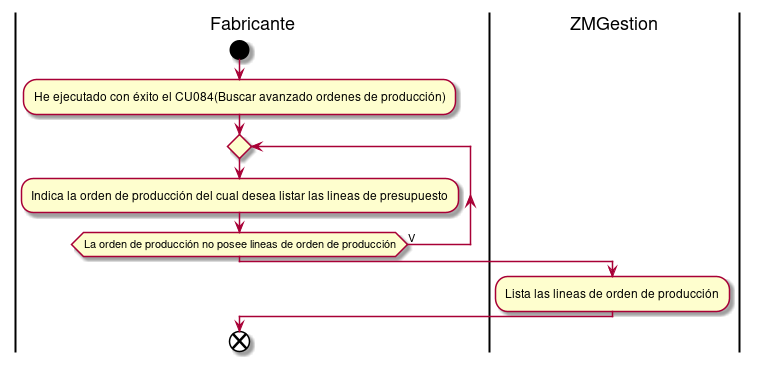
\includegraphics[width=\textwidth,height=0.95\textheight,keepaspectratio]{DiagramasActividad/DiagramaDeActividad/listarLineasOrdenProduccion}
    \caption{CU94 - Listar líneas de orden de producción}
\label{fig:listarLineasOrdenProduccion}
\end{figure}
		
\renewcommand{\caseUseShortName}{cancelarOrdenProduccion} %cammelCase name

\renewcommand{\caseUseCreated}{05/03/2020} %Fecha creación
\renewcommand{\caseUseModified}{05/03/2020} %Fecha modificación
\renewcommand{\caseUseName}{\CUcancelarOrdenProduccion - Cancelar orden de producción} %{\CUcammelCase - Title}

\renewcommand{\caseUseSummary}{Este caso de uso permite a un administrador de ZMGestion cancelar una orden de producción.} %Resumen
\renewcommand{\caseUsePeople}{Administradores: quiere cancelar una orden de producción existente.} %Actor: Meta
\renewcommand{\caseUsePreconditions}{
	\caseUseRow{Haber realizado con éxito el \CUbuscarAvanzadoOrdenesProduccion\ (Buscar avanzado órdenes de producción).}
}
\renewcommand{\caseUsePostconditions}{
	\caseUseRow{Ninguna.} %Postcondiciones
}
\renewcommand{\caseUseScene}{ %Escenario principal
    \addCaseUseStep{El administrador selecciona una orden de producción que desea cancelar.}
    \addCaseUseStep{ZMGestion ejecuta el \CUcancelarLineaOrdenProduccion\ (Cancelar línea orden de producción) para cada línea de la orden de producción que se encuentre `Pendiente de producción' o `En producción'.}
}
\renewcommand{\alternativeCaseUse}{ %Flujos alternativos
	\newAlternative{A1: La orden de producción seleccionada no se encuentra en estado `Pendiente' o `En producción'.}{1} %Flujo alternativo A1.
	\caseUseRow{La secuencia A1 comienza luego del punto 1 del escenario principal.} %¡Indicar número paso!
    \alternativeRow{ZMGestion muestra un mensaje de error indicando que la orden de producción no puede cancelarse.}
    \caseUseRow{El escenario vuelve al punto 1.}
    \caseUseRow{}
}

%\item Caso de uso \caseUseName
\input{Capitulos/Capitulo4/CasosUso/generalTable.tex}

%DIAGRAMA DE ACTIVIDAD
%\lineabreak[0]
\activityDiagram{\caseUseShortName}{Diagrama de actividad - \caseUseName}
		
\renewcommand{\caseUseShortName}{listarLineasOrdenProduccion} %cammelCase name

\renewcommand{\caseUseCreated}{03/03/2020} %Fecha creación
\renewcommand{\caseUseModified}{03/03/2020} %Fecha modificación
\renewcommand{\caseUseName}{\CUlistarLineasOrdenProduccion - Listar lineas de orden de producción } %{\CUcammelCase - Title}

\renewcommand{\caseUseSummary}{Este caso de uso permite a los usuarios de ZMGestion listar las lineas de orden de producción de una orden de producción especifica.} %Resumen
\renewcommand{\caseUsePeople}{Usuarios: quiere listar las lineas de orden de producción.} %Actor: Meta
\renewcommand{\caseUsePreconditions}{\caseUseRow{Haber realizado con éxito el \CUbuscarAvanzadoOrdenesProduccion\ (Buscar avanzado órdenes de producción).} %Precondiciones
}
\renewcommand{\caseUsePostconditions}{
	\caseUseRow{Ninguna.} %Postcondiciones
}
\renewcommand{\caseUseScene}{ %Escenario principal
    \addCaseUseStep{El usuario indica la orden de producción de la cual desea listar sus lineas de orden de producción.}
    \addCaseUseStep{ZMGestion lista las lineas de orden de producción de la orden de producción seleccionada.}
}
\renewcommand{\alternativeCaseUse}{ %Flujos alternativos
	\newAlternative{A1: La orden de producción no posee lineas de orden de producción.}{1} %Flujo alternativo A1.
	\caseUseRow{La secuencia A1 comienza luego del punto 1 del escenario principal.} %¡Indicar número paso!
    \alternativeRow{ZMGestion muetsra un mensaje indicando que la orden de producción indicada no posee lineas de orden de producción.}
    \caseUseRow{El escenario vuelve al punto 1.}
    \caseUseRow{}

}
\renewcommand{\caseUseRequirementsGUI}{
	\caseUseRow{Teclado, Mouse y Pantalla} %Requisitos interfaz de usuario
}
\renewcommand{\caseUseResponseTime}{La interfaz debe responder dentro de un tiempo máximo de 10 segundos.} %Requisitos funcionales: Tiempo de respuesta
\renewcommand{\caseUseConcurrence}{} %Requisitos funcionales: Concurrencia
\renewcommand{\caseUseAvailability}{} %Requisitos funcionales: Disponibilidad

\item Caso de uso \caseUseName
\input{Capitulos/Capitulo4/CasosUso/generalTable.tex}

%DIAGRAMA DE ACTIVIDAD
%\lineabreak[0]
%\activityDiagram{\caseUseShortName}{Diagrama de actividad - \caseUseName}

		%GestionLineasOrdenesProduccion
		
\renewcommand{\caseUseShortName}{verificarLineaOrdenProduccion} %cammelCase name

\renewcommand{\caseUseCreated}{04/03/2020} %Fecha creación
\renewcommand{\caseUseModified}{04/03/2020} %Fecha modificación
\renewcommand{\caseUseName}{\CUverificarLineaOrdenProduccion - Verificar línea de orden de producción} %{\CUcammelCase - Title}

\renewcommand{\caseUseSummary}{Este caso de uso permite a un administrador de ZMGestion verificar que una línea de orden de producción (cuyas tareas se encuentran finalizadas) efectivamente se ha finalizado.} %Resumen
\renewcommand{\caseUsePeople}{Administradores: quiere verificar que una línea de orden de producción está finalizada.} %Actor: Meta
\renewcommand{\caseUsePreconditions}{
	\caseUseRow{Haber ejecutado con éxito el \CUlistarLineasOrdenProduccion (Listar lineas de orden de producción).} %Precondiciones
}
\renewcommand{\caseUsePostconditions}{
	\caseUseRow{Ninguna.} %Postcondiciones
}
\renewcommand{\caseUseScene}{ %Escenario principal
    \addCaseUseStep{El administrador indica la línea de orden de producción que desea verificar que esta finalizada.}
    \addCaseUseStep{ZMGestion pasa la línea de orden de producción al estado `Verificada' y en caso de tener una venta asociada reserva los productos fabricados para el cliente, pasando las lineas de venta utilizadas para generar la orden de produccion al estado `Reservada'.}
}
\renewcommand{\alternativeCaseUse}{ %Flujos alternativos
	\newAlternative{A1: La línea de orden de producción no se encuentra en estado `En producción' o sus tareas no están todas finalizadas.}{1} %Flujo alternativoA1.
	\caseUseRow{La secuencia A1 comienza luego del punto 1 del escenario principal.} %¡Indicar número paso!
    \alternativeRow{ZMGestion muestra un mensaje de error indicando que la línea de orden de producción no puede ser verificada.}
    \caseUseRow{El escenario vuelve al punto 1.}    
    \caseUseRow{}
}

%\item Caso de uso \caseUseName
\input{Capitulos/Capitulo4/CasosUso/generalTable.tex}

%DIAGRAMA DE ACTIVIDAD
%\lineabreak[0]
%\activityDiagram{\caseUseShortName}{Diagrama de actividad - \caseUseName}
		
\renewcommand{\caseUseShortName}{} %cammelCase name

\renewcommand{\caseUseCreated}{15/02/2020} %Fecha creación
\renewcommand{\caseUseModified}{15/02/2020} %Fecha modificación
\renewcommand{\caseUseName}{\CU - } %{\CUcammelCase - Title}

\renewcommand{\caseUseSummary}{} %Resumen
\renewcommand{\caseUsePeople}{} %Actor: Meta
\renewcommand{\caseUsePreconditions}{
	\caseUseRow{Haber iniciado sesión en el sistema.} %Precondiciones
}
\renewcommand{\caseUsePostconditions}{
	\caseUseRow{Ninguna.} %Postcondiciones
}
\renewcommand{\caseUseScene}{ %Escenario principal
    \addCaseUseStep{}
    \addCaseUseStep{}
    \addCaseUseStep{}
    \addCaseUseStep{}
    \addCaseUseStep{}
    \addCaseUseStep{}
    \addCaseUseStep{}
    \addCaseUseStep{}
}
\renewcommand{\alternativeCaseUse}{ %Flujos alternativos
	\newAlternative{A1: Error al .}{NUMERO} %Flujo alternativo A1.
	\caseUseRow{La secuencia A1 comienza luego del punto NUMERO del escenario principal.} %¡Indicar número paso!
    \alternativeRow{}
    \alternativeRow{}
    \alternativeRow{}
    \alternativeRow{}
    \alternativeRow{}
    \alternativeRow{}
    
    \caseUseRow{}

	\newAlternative{A2: Error al .}{NUMERO} %Flujo alternativo A2.
    \caseUseRow{La secuencia A2 comienza luego del punto NUMERO del escenario principal.}%¡Indicar número paso!
    \alternativeRow{}
    \alternativeRow{}
    \alternativeRow{}
    \alternativeRow{}
    \alternativeRow{}
    \alternativeRow{}
}
\renewcommand{\caseUseRequirementsGUI}{
	\caseUseRow{Teclado, Mouse y Pantalla} %Requisitos interfaz de usuario
}
\renewcommand{\caseUseResponseTime}{La interfaz debe responder dentro de un tiempo máximo de 10 segundos.} %Requisitos funcionales: Tiempo de respuesta
\renewcommand{\caseUseConcurrence}{} %Requisitos funcionales: Concurrencia
\renewcommand{\caseUseAvailability}{} %Requisitos funcionales: Disponibilidad

\item Caso de uso \caseUseName
\input{Capitulos/Capitulo4/CasosUso/generalTable.tex}

%DIAGRAMA DE ACTIVIDAD
%\lineabreak[0]
%\activityDiagram{\caseUseShortName}{Diagrama de actividad - \caseUseName}
		
\renewcommand{\caseUseShortName}{reanudarLineaOrdenProduccion} %cammelCase name

\renewcommand{\caseUseCreated}{05/03/2020} %Fecha creación
\renewcommand{\caseUseModified}{05/03/2020} %Fecha modificación
\renewcommand{\caseUseName}{\CUreanudarLineaOrdenProduccion - Reanudar línea de orden de producción} %{\CUcammelCase - Title}

\renewcommand{\caseUseSummary}{Este caso de uso permite a un administrador de ZMGestion reanudar la producción de una línea de orden de producción que fue cancelada.} %Resumen

\renewcommand{\caseUsePeople}{Administradores: quiere reanudar la producción de una línea de orden de producción cancelada.} %Actor: Meta
\renewcommand{\caseUsePreconditions}{
	\caseUseRow{Haber ejecutado con éxito el \CUlistarLineasOrdenProduccion (Listar lineas de orden de producción).} %Precondiciones
}
\renewcommand{\caseUsePostconditions}{
	\caseUseRow{Ninguna.} %Postcondiciones
}
\renewcommand{\caseUseScene}{ %Escenario principal
    \addCaseUseStep{El administrador indica la línea de orden de producción que desea reanudar.}
    \addCaseUseStep{Si la línea de orden de producción tiene tareas ZMGestion cambia el estado de la línea de orden de producción al estado de `En producción', caso contrario al estado de `Pendiente de producción'. ZMGestion muestra un mensaje indicando el éxito de la operación.}
}
\renewcommand{\alternativeCaseUse}{ %Flujos alternativos
    \newAlternative{A1: La línea de orden de producción no se encuentra en estado de `Cancelada'.}{1} %Flujo alternativo A1.
    \caseUseRow{La secuencia A1 comienza luego del punto 1 del escenario principal.} %¡Indicar número paso!
    \alternativeRow{ZMGestion muestra un mensaje de error indicando que la línea de orden de producción no puede reanudarse.}
    \caseUseRow{el escenario vuelve al punto 1.}
    \caseUseRow{}
}
%\item Caso de uso \caseUseName
\input{Capitulos/Capitulo4/CasosUso/generalTable.tex}

%DIAGRAMA DE ACTIVIDAD
%\lineabreak[0]
%\activityDiagram{\caseUseShortName}{Diagrama de actividad - \caseUseName}
		
		%GestionTareas
		
\renewcommand{\caseUseShortName}{} %cammelCase name

\renewcommand{\caseUseCreated}{15/02/2020} %Fecha creación
\renewcommand{\caseUseModified}{15/02/2020} %Fecha modificación
\renewcommand{\caseUseName}{\CU - } %{\CUcammelCase - Title}

\renewcommand{\caseUseSummary}{} %Resumen
\renewcommand{\caseUsePeople}{} %Actor: Meta
\renewcommand{\caseUsePreconditions}{
	\caseUseRow{Haber iniciado sesión en el sistema.} %Precondiciones
}
\renewcommand{\caseUsePostconditions}{
	\caseUseRow{Ninguna.} %Postcondiciones
}
\renewcommand{\caseUseScene}{ %Escenario principal
    \addCaseUseStep{}
    \addCaseUseStep{}
    \addCaseUseStep{}
    \addCaseUseStep{}
    \addCaseUseStep{}
    \addCaseUseStep{}
    \addCaseUseStep{}
    \addCaseUseStep{}
}
\renewcommand{\alternativeCaseUse}{ %Flujos alternativos
	\newAlternative{A1: Error al .}{NUMERO} %Flujo alternativo A1.
	\caseUseRow{La secuencia A1 comienza luego del punto NUMERO del escenario principal.} %¡Indicar número paso!
    \alternativeRow{}
    \alternativeRow{}
    \alternativeRow{}
    \alternativeRow{}
    \alternativeRow{}
    \alternativeRow{}
    
    \caseUseRow{}

	\newAlternative{A2: Error al .}{NUMERO} %Flujo alternativo A2.
    \caseUseRow{La secuencia A2 comienza luego del punto NUMERO del escenario principal.}%¡Indicar número paso!
    \alternativeRow{}
    \alternativeRow{}
    \alternativeRow{}
    \alternativeRow{}
    \alternativeRow{}
    \alternativeRow{}
}
\renewcommand{\caseUseRequirementsGUI}{
	\caseUseRow{Teclado, Mouse y Pantalla} %Requisitos interfaz de usuario
}
\renewcommand{\caseUseResponseTime}{La interfaz debe responder dentro de un tiempo máximo de 10 segundos.} %Requisitos funcionales: Tiempo de respuesta
\renewcommand{\caseUseConcurrence}{} %Requisitos funcionales: Concurrencia
\renewcommand{\caseUseAvailability}{} %Requisitos funcionales: Disponibilidad

\item Caso de uso \caseUseName
\input{Capitulos/Capitulo4/CasosUso/generalTable.tex}

%DIAGRAMA DE ACTIVIDAD
%\lineabreak[0]
%\activityDiagram{\caseUseShortName}{Diagrama de actividad - \caseUseName}
		\renewcommand{\caseUseShortName}{borrarTarea} %cammelCase name

\renewcommand{\caseUseCreated}{05/03/2020} %Fecha creación
\renewcommand{\caseUseModified}{05/03/2020} %Fecha modificación
\renewcommand{\caseUseName}{\CUborrarTarea - Borrar tarea} %{\CUcammelCase - Title}

\renewcommand{\caseUseSummary}{Este caso de uso permite a un administrador de ZMGestion borrar una tarea de una línea de orden de producción existente.} %Resumen
\renewcommand{\caseUsePeople}{Administradores: quiere borrar una tarea de una línea de orden de producción.} %Actor: Meta
\renewcommand{\caseUsePreconditions}{
	\caseUseRow{Haber ejecutado con éxito el \CUlistarTareasLineaOrdenProduccion (Listar tareas de línea de orden de producción).} %Precondiciones
}
\renewcommand{\caseUsePostconditions}{
	\caseUseRow{Ninguna.} %Postcondiciones
}
\renewcommand{\caseUseScene}{ %Escenario principal
    \addCaseUseStep{El administrador indica la tarea de la línea de orden de producción que desea borrar.}
    \addCaseUseStep{ZMGestion borra la tarea de la linea de orden de producción.}
}
\renewcommand{\alternativeCaseUse}{ %Flujos alternativos
	\newAlternative{A1: La tarea no se encuentra en estado `Pendiente' o `Cancelada'.}{1} %Flujo alternativo A2.
	\caseUseRow{La secuencia A1 comienza luego del punto 1 del escenario principal.} %¡Indicar número paso!
    \alternativeRow{ZMGestion muestra un mensaje de error indicando que no se puede borrar la tarea.}
    \caseUseRow{El escenario vuelve al punto 1.}    
    \caseUseRow{}
}

%\item Caso de uso \caseUseName
\input{Capitulos/Capitulo4/CasosUso/generalTable.tex}

%DIAGRAMA DE ACTIVIDAD
%\lineabreak[0]
%\activityDiagram{\caseUseShortName}{Diagrama de actividad - \caseUseName}
		\renewcommand{\caseUseShortName}{finalizarTarea} %cammelCase name

\renewcommand{\caseUseCreated}{05/03/2020} %Fecha creación
\renewcommand{\caseUseModified}{05/03/2020} %Fecha modificación
\renewcommand{\caseUseName}{\CUfinalizarTarea - Finalizar tarea} %{\CUcammelCase - Title}

\renewcommand{\caseUseSummary}{Este caso de uso permite a un fabricante de ZMGestion indicar que se ha finalizado una tarea de una línea de orden de producción existente.} %Resumen
\renewcommand{\caseUsePeople}{Fabricantes: quiere indicar que ha finalizado la ejecución de una tarea en una línea de orden de producción.} %Actor: Meta
\renewcommand{\caseUsePreconditions}{
	\caseUseRow{Haber ejecutado con éxito el CU97 (Listar tareas de línea de orden de producción).} %Precondiciones
}
\renewcommand{\caseUsePostconditions}{
	\caseUseRow{Ninguna.} %Postcondiciones
}
\renewcommand{\caseUseScene}{ %Escenario principal
    \addCaseUseStep{El fabricante indica la tarea, de una línea de orden de producción, que ha finalizado.}
    \addCaseUseStep{ZMGestion pasa el estado de la tarea seleccionada a `Finalizada'.}
}
\renewcommand{\alternativeCaseUse}{ %Flujos alternativos
	\newAlternative{A1: La tarea no se encuentra en estado `En proceso'.}{1} %Flujo alternativo A2.
	\caseUseRow{La secuencia A1 comienza luego del punto 1 del escenario principal.} %¡Indicar número paso!
    \alternativeRow{ZMGestion muestra un mensaje de error indicando que no se puede finalizar una tarea que no está en proceso.}
    \caseUseRow{El escenario vuelve al punto 1.}    
    \caseUseRow{}
}

%\item Caso de uso \caseUseName
\input{Capitulos/Capitulo4/CasosUso/generalTable.tex}

%DIAGRAMA DE ACTIVIDAD
%\lineabreak[0]
%\activityDiagram{\caseUseShortName}{Diagrama de actividad - \caseUseName}
		\renewcommand{\caseUseShortName}{verificarTarea} %cammelCase name

\renewcommand{\caseUseCreated}{05/03/2020} %Fecha creación
\renewcommand{\caseUseModified}{05/03/2020} %Fecha modificación
\renewcommand{\caseUseName}{\CUverificarTarea - Verificar tarea} %{\CUcammelCase - Title}

\renewcommand{\caseUseSummary}{Este caso de uso permite a un administrador de ZMGestion verificar la finalización de una tarea que fue asignada previamente como finalizada por un fabricante.} %Resumen
\renewcommand{\caseUsePeople}{Administradores: quiere verificar la finalización de una tarea.} %Actor: Meta
\renewcommand{\caseUsePreconditions}{
	\caseUseRow{Haber ejecutado con éxito el CU97 (Listar tareas de línea de orden de producción).} %Precondiciones
}
\renewcommand{\caseUsePostconditions}{
	\caseUseRow{Ninguna.} %Postcondiciones
}
\renewcommand{\caseUseScene}{ %Escenario principal
    \addCaseUseStep{El administrador indica la tarea de una línea de orden de producción que desea verificar su finalización.}
    \addCaseUseStep{ZMGestion pasa el estado de la tarea seleccionada a `Verificada'.}
}
\renewcommand{\alternativeCaseUse}{ %Flujos alternativos
	\newAlternative{A1: La tarea no se encuentra en estado `Finalizada'.}{1} %Flujo alternativo A2.
	\caseUseRow{La secuencia A1 comienza luego del punto 1 del escenario principal.} %¡Indicar número paso!
    \alternativeRow{ZMGestion muestra un mensaje de error indicando que no se puede verificar la finalización de una tarea que no se ha finalizado.}
    \caseUseRow{El escenario vuelve al punto 1.}    
    \caseUseRow{}
}

%\item Caso de uso \caseUseName
\input{Capitulos/Capitulo4/CasosUso/generalTable.tex}

%DIAGRAMA DE ACTIVIDAD
%\lineabreak[0]
%\activityDiagram{\caseUseShortName}{Diagrama de actividad - \caseUseName}
		\renewcommand{\caseUseShortName}{pausarTarea} %cammelCase name

\renewcommand{\caseUseCreated}{05/03/2020} %Fecha creación
\renewcommand{\caseUseModified}{05/03/2020} %Fecha modificación
\renewcommand{\caseUseName}{\CUpausarTarea - Pausar tarea} %{\CUcammelCase - Title}

\renewcommand{\caseUseSummary}{Este caso de uso permite a un administrador de ZMGestion pausar la ejecución de una tarea en una línea de orden de producción existente.} %Resumen
\renewcommand{\caseUsePeople}{Administradores: quiere pausar la ejecución de una tarea en una línea de orden de producción.} %Actor: Meta
\renewcommand{\caseUsePreconditions}{
	\caseUseRow{Haber ejecutado con éxito el CU97 (Listar tareas de línea de orden de producción).} %Precondiciones
}
\renewcommand{\caseUsePostconditions}{
	\caseUseRow{Ninguna.} %Postcondiciones
}
\renewcommand{\caseUseScene}{ %Escenario principal
    \addCaseUseStep{El administrador indica una tarea de una línea de orden de producción a la cual le desea pausar su ejecución.}
    \addCaseUseStep{ZMGestion pasa el estado de la tarea seleccionada a `Pausada'.}
}
\renewcommand{\alternativeCaseUse}{ %Flujos alternativos
	\newAlternative{A1: La tarea no se encuentra en estado `En proceso', `Finalizada' o `Pausada'.}{1} %Flujo alternativo A2.
	\caseUseRow{La secuencia A1 comienza luego del punto 1 del escenario principal.} %¡Indicar número paso!
    \alternativeRow{ZMGestion muestra un mensaje de error indicando que la tarea no se puede cancelar.}
    \caseUseRow{El escenario vuelve al punto 1.}    
    \caseUseRow{}
}

%\item Caso de uso \caseUseName
\input{Capitulos/Capitulo4/CasosUso/generalTable.tex}

%DIAGRAMA DE ACTIVIDAD
%\lineabreak[0]
%\activityDiagram{\caseUseShortName}{Diagrama de actividad - \caseUseName}
		\renewcommand{\caseUseShortName}{reanudarTarea} %cammelCase name

\renewcommand{\caseUseCreated}{05/03/2020} %Fecha creación
\renewcommand{\caseUseModified}{05/03/2020} %Fecha modificación
\renewcommand{\caseUseName}{\CUreanudarTarea - Reanudar tarea} %{\CUcammelCase - Title}

\renewcommand{\caseUseSummary}{Este caso de uso permite a un administrador de ZMGestion reanudar la ejecución de una tarea en una línea de orden de producción existente.} %Resumen
\renewcommand{\caseUsePeople}{Administradores: quiere reanudar la ejecución de una tarea en una línea de orden de producción.} %Actor: Meta
\renewcommand{\caseUsePreconditions}{
	\caseUseRow{Haber ejecutado con éxito el \CUlistarTareasLineaOrdenProduccion (Listar tareas de línea de orden de producción).} %Precondiciones
}
\renewcommand{\caseUsePostconditions}{
	\caseUseRow{Ninguna.} %Postcondiciones
}
\renewcommand{\caseUseScene}{ %Escenario principal
    \addCaseUseStep{El administrador indica una tarea de una línea de orden de producción a la cual le desea reanudar su ejecución.}
    \addCaseUseStep{ZMGestion pasa el estado de la tarea seleccionada a `En proceso'.}
}
\renewcommand{\alternativeCaseUse}{ %Flujos alternativos
	\newAlternative{A1: La tarea no se encuentra en estado `Pausada', `Finalizada' o `Cancelada'.}{1} %Flujo alternativo A2.
	\caseUseRow{La secuencia A1 comienza luego del punto 1 del escenario principal.} %¡Indicar número paso!
    \alternativeRow{ZMGestion muestra un mensaje de error indicando que la tarea no se puede reanudar.}
    \caseUseRow{El escenario vuelve al punto 1.}    
    \caseUseRow{}
}

\item Caso de uso \caseUseName
\input{Capitulos/Capitulo4/CasosUso/generalTable.tex}

%DIAGRAMA DE ACTIVIDAD
%\lineabreak[0]
%\activityDiagram{\caseUseShortName}{Diagrama de actividad - \caseUseName}
		
\renewcommand{\caseUseShortName}{} %cammelCase name

\renewcommand{\caseUseCreated}{15/02/2020} %Fecha creación
\renewcommand{\caseUseModified}{15/02/2020} %Fecha modificación
\renewcommand{\caseUseName}{\CU - } %{\CUcammelCase - Title}

\renewcommand{\caseUseSummary}{} %Resumen
\renewcommand{\caseUsePeople}{} %Actor: Meta
\renewcommand{\caseUsePreconditions}{
	\caseUseRow{Haber iniciado sesión en el sistema.} %Precondiciones
}
\renewcommand{\caseUsePostconditions}{
	\caseUseRow{Ninguna.} %Postcondiciones
}
\renewcommand{\caseUseScene}{ %Escenario principal
    \addCaseUseStep{}
    \addCaseUseStep{}
    \addCaseUseStep{}
    \addCaseUseStep{}
    \addCaseUseStep{}
    \addCaseUseStep{}
    \addCaseUseStep{}
    \addCaseUseStep{}
}
\renewcommand{\alternativeCaseUse}{ %Flujos alternativos
	\newAlternative{A1: Error al .}{NUMERO} %Flujo alternativo A1.
	\caseUseRow{La secuencia A1 comienza luego del punto NUMERO del escenario principal.} %¡Indicar número paso!
    \alternativeRow{}
    \alternativeRow{}
    \alternativeRow{}
    \alternativeRow{}
    \alternativeRow{}
    \alternativeRow{}
    
    \caseUseRow{}

	\newAlternative{A2: Error al .}{NUMERO} %Flujo alternativo A2.
    \caseUseRow{La secuencia A2 comienza luego del punto NUMERO del escenario principal.}%¡Indicar número paso!
    \alternativeRow{}
    \alternativeRow{}
    \alternativeRow{}
    \alternativeRow{}
    \alternativeRow{}
    \alternativeRow{}
}
\renewcommand{\caseUseRequirementsGUI}{
	\caseUseRow{Teclado, Mouse y Pantalla} %Requisitos interfaz de usuario
}
\renewcommand{\caseUseResponseTime}{La interfaz debe responder dentro de un tiempo máximo de 10 segundos.} %Requisitos funcionales: Tiempo de respuesta
\renewcommand{\caseUseConcurrence}{} %Requisitos funcionales: Concurrencia
\renewcommand{\caseUseAvailability}{} %Requisitos funcionales: Disponibilidad

\item Caso de uso \caseUseName
\input{Capitulos/Capitulo4/CasosUso/generalTable.tex}

%DIAGRAMA DE ACTIVIDAD
%\lineabreak[0]
%\activityDiagram{\caseUseShortName}{Diagrama de actividad - \caseUseName}
		\renewcommand{\caseUseShortName}{ejecutarTarea} %cammelCase name

\renewcommand{\caseUseCreated}{05/03/2020} %Fecha creación
\renewcommand{\caseUseModified}{05/03/2020} %Fecha modificación
\renewcommand{\caseUseName}{\CUejecutarTarea - Ejecutar tarea} %{\CUcammelCase - Title}

\renewcommand{\caseUseSummary}{Este caso de uso permite a un fabricante de ZMGestion indicar que se está por iniciar la ejecución de una tarea que se le asignó en una línea de orden de producción.} %Resumen
\renewcommand{\caseUsePeople}{Fabricantes: quiere indicar que iniciará la ejecución de una tarea que se le asignó en una línea de orden de producción.} %Actor: Meta
\renewcommand{\caseUsePreconditions}{
	\caseUseRow{Haber ejecutado con éxito el CU97 (Listar tareas de línea de orden de producción).} %Precondiciones
}
\renewcommand{\caseUsePostconditions}{
	\caseUseRow{Ninguna.} %Postcondiciones
}
\renewcommand{\caseUseScene}{ %Escenario principal
    \addCaseUseStep{El fabricante indica la tarea que iniciará, de una línea de orden de producción.}
    \addCaseUseStep{ZMGestion pasa el estado de la tarea seleccionada a `En proceso'.}
}
\renewcommand{\alternativeCaseUse}{ %Flujos alternativos
	\newAlternative{A1: La tarea no se encuentra en estado `Pendiente'.}{1} %Flujo alternativo A1.
	\caseUseRow{La secuencia A1 comienza luego del punto 1 del escenario principal.} %¡Indicar número paso!
    \alternativeRow{ZMGestion muestra un mensaje de error indicando que la tarea ya se inició previamente.}
    \caseUseRow{El escenario vuelve al punto 1.}    
    \caseUseRow{}
    \newAlternative{A2: La tarea indicada no se le asignó al fabricante que está intentando ejecutarla.}{1} %Flujo alternativo A2.
	\caseUseRow{La secuencia A2 comienza luego del punto 1 del escenario principal.} %¡Indicar número paso!
    \alternativeRow{ZMGestion muestra un mensaje de error indicando que la tarea no se le asignó a el.}
    \caseUseRow{El escenario vuelve al punto 1.}    
    \caseUseRow{}
}

%\item Caso de uso \caseUseName
\input{Capitulos/Capitulo4/CasosUso/generalTable.tex}

%DIAGRAMA DE ACTIVIDAD
%\lineabreak[0]
%\activityDiagram{\caseUseShortName}{Diagrama de actividad - \caseUseName}

	\subsection{Diagrama de clases}
	\begin{figure}[H]
		\centering
		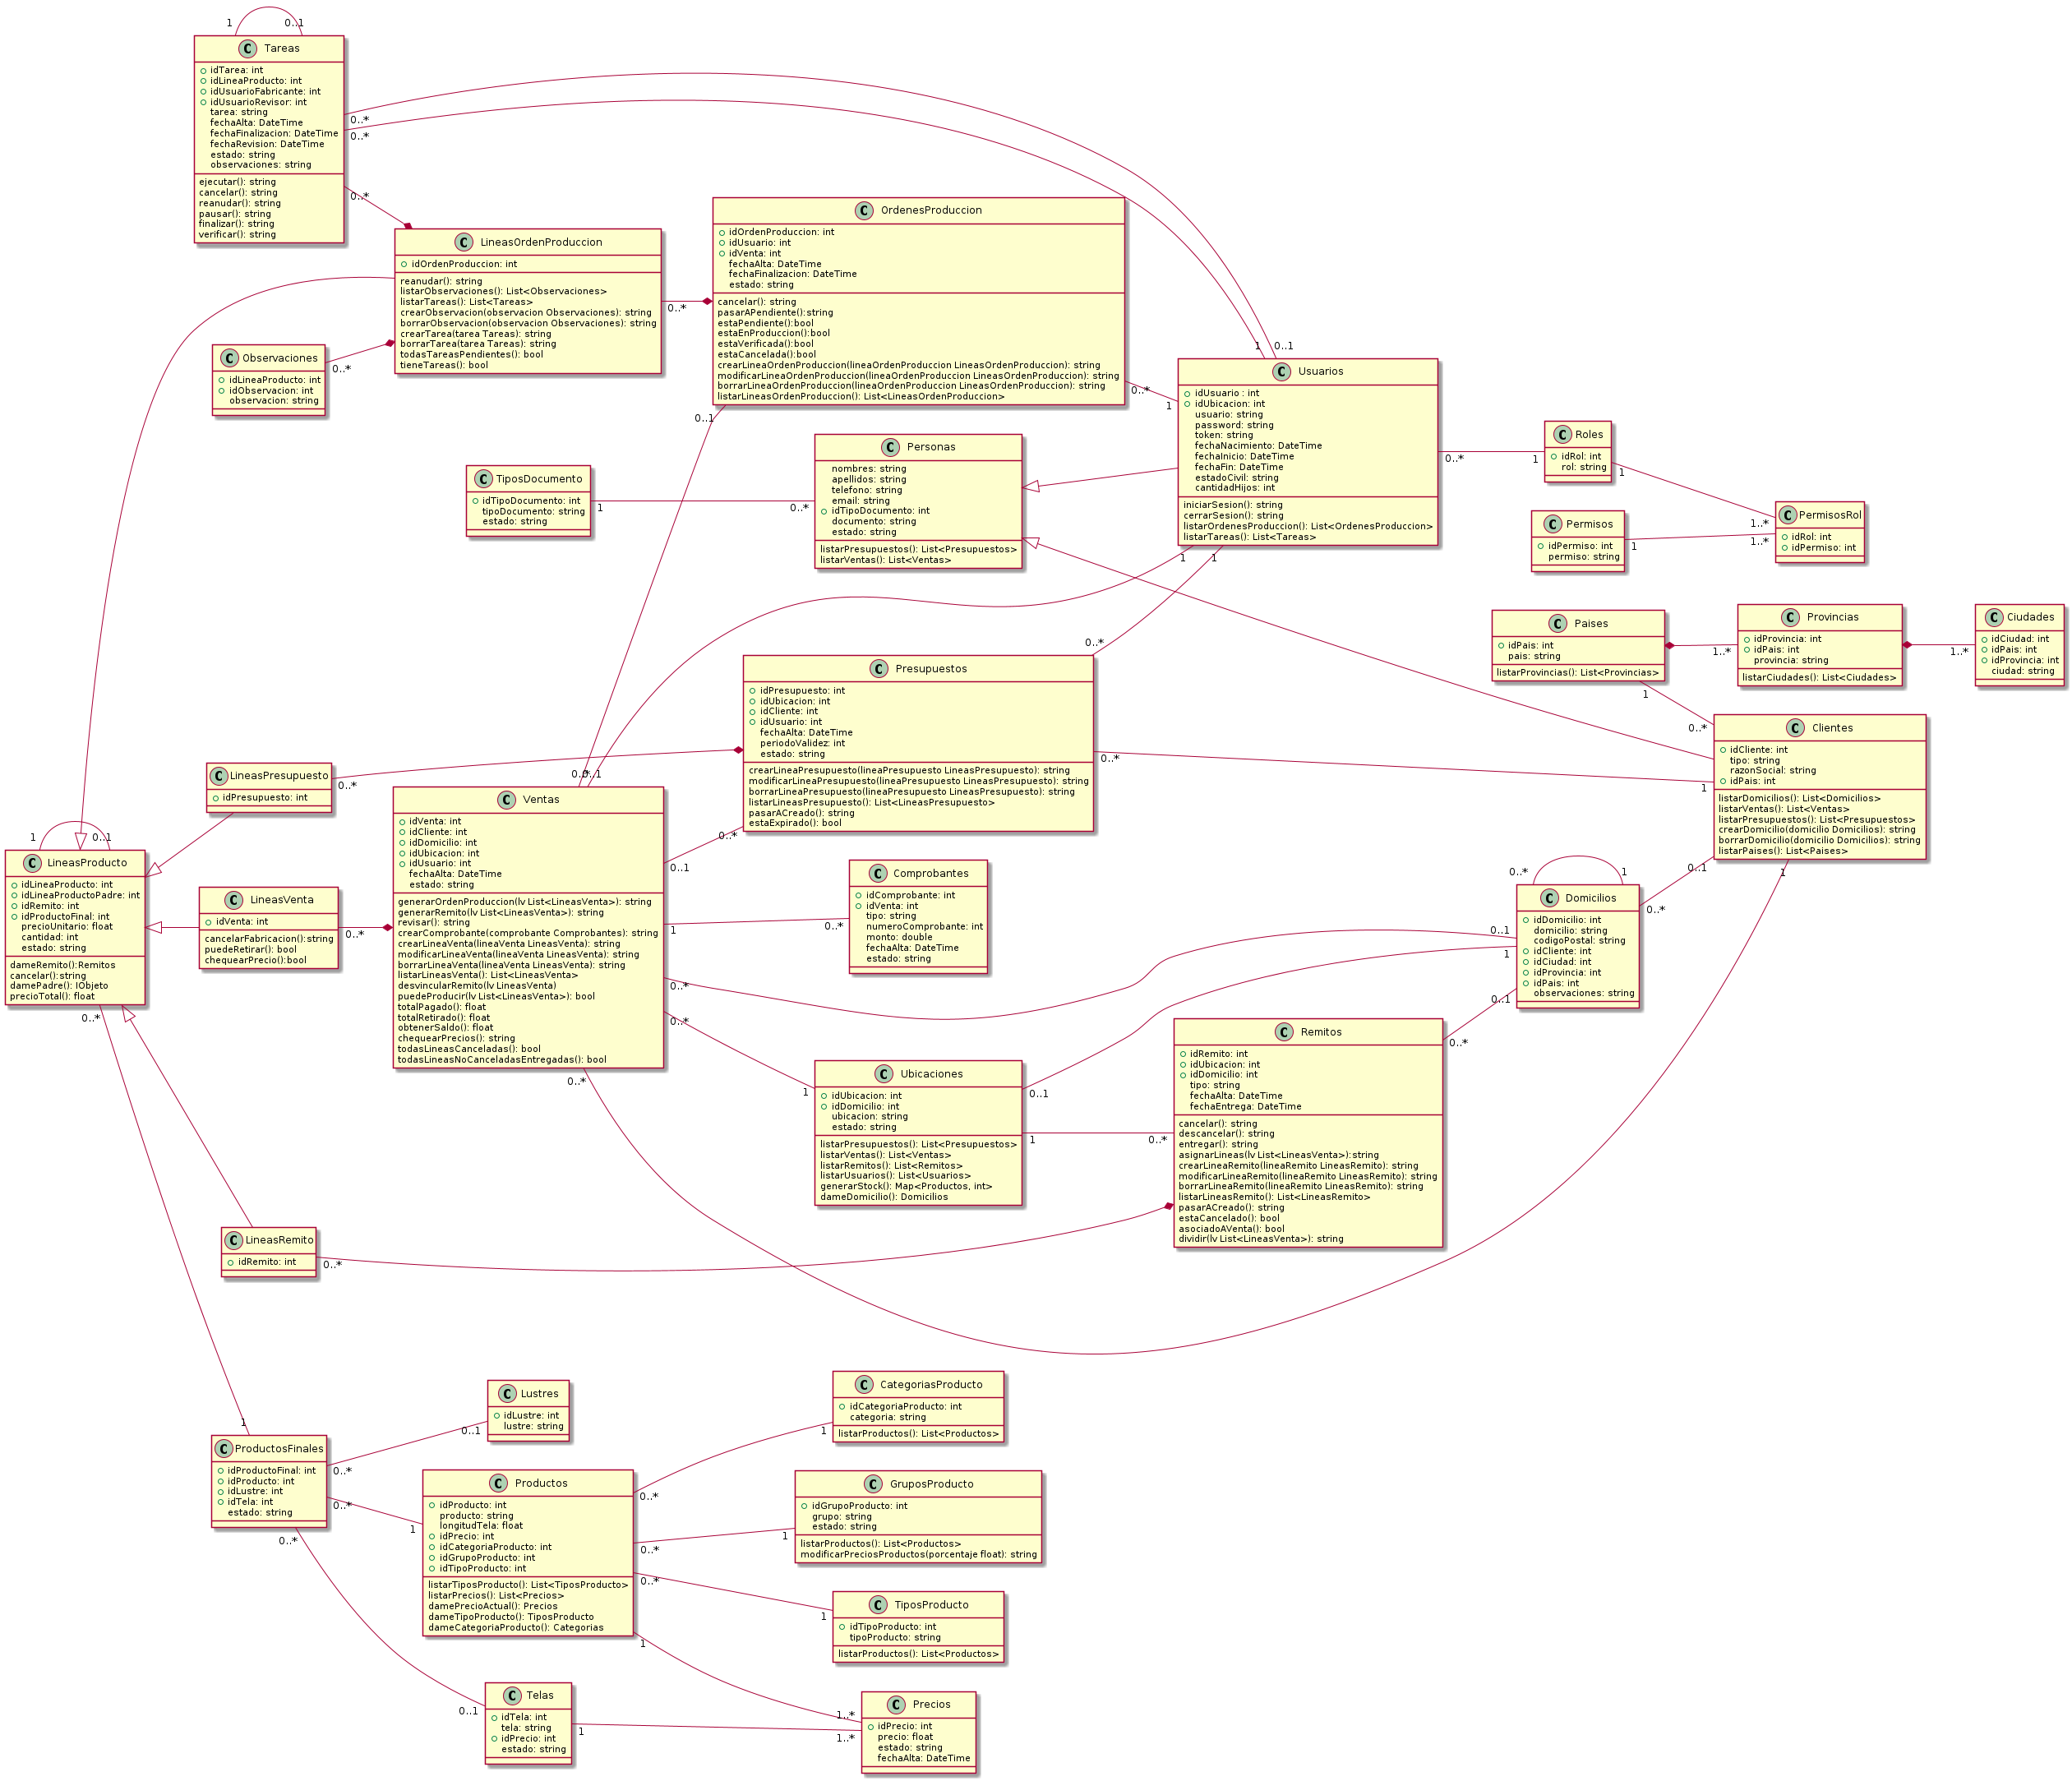
\includegraphics[width=\textwidth,height=\textheight,keepaspectratio]{DiagramaClases/Vistas/diagramaClases}
		\caption{Diagrama de clases}
	\label{fig:Diagrama de clases}
	\end{figure}
	\clearpage %salto de pagina

	\begin{figure}[H]
		\centering
		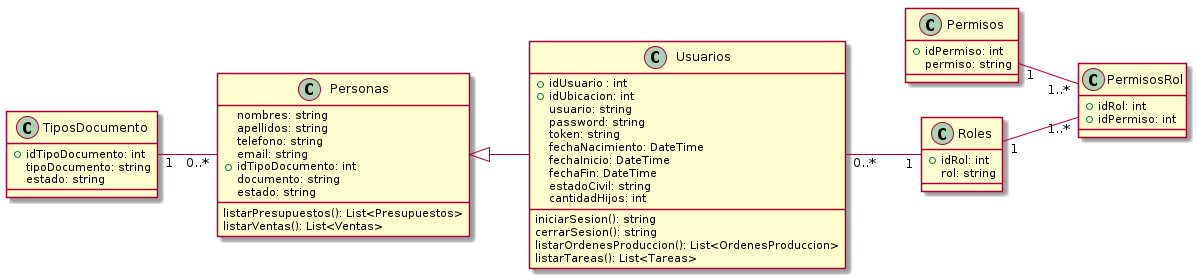
\includegraphics[width=\textwidth,height=\textheight,keepaspectratio]{DiagramaClases/Vistas/vistaSistema}
		\caption{Diagrama de clases - Vista sistema}
	\label{fig:Diagrama de clases - Vista sistema}
	\end{figure}

	\begin{figure}[H]
		\centering
		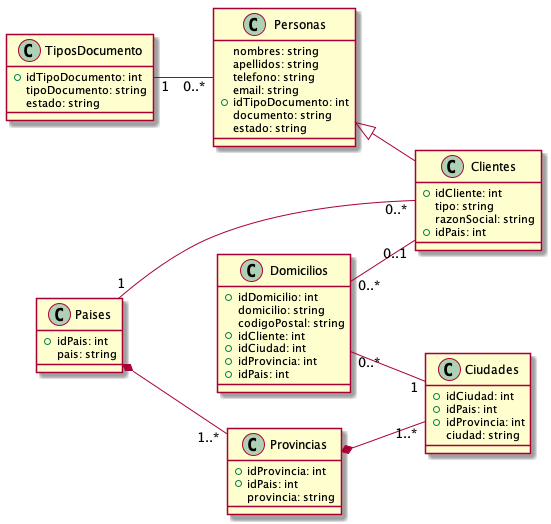
\includegraphics[width=\textwidth,height=0.90\textheight,keepaspectratio]{DiagramaClases/Vistas/vistaClientes}
		\caption{Diagrama de clases - Vista clientes}
	\label{fig:Diagrama de clases - Vista clientes}
    \end{figure}
	\begin{figure}[H]
		\centering
		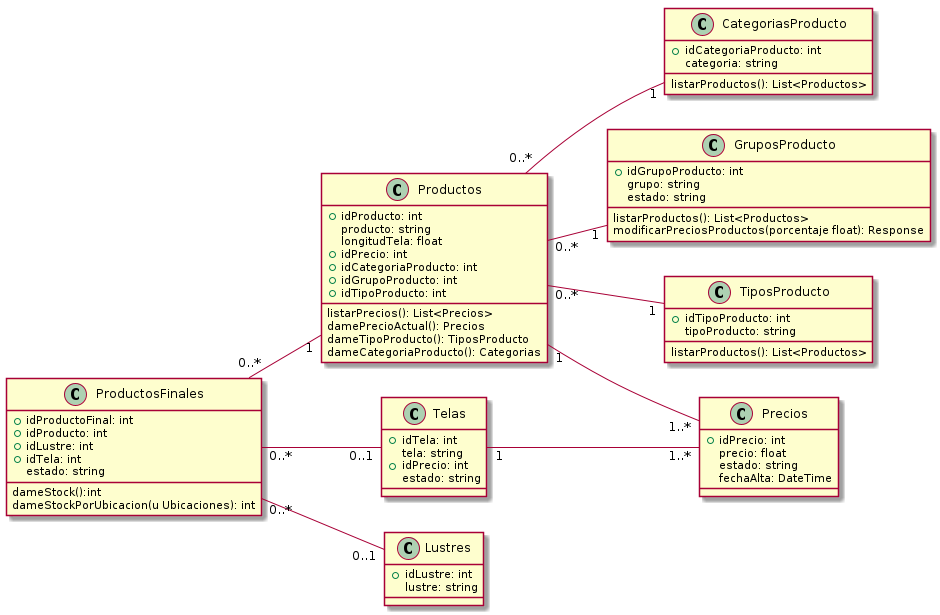
\includegraphics[width=\textwidth,height=0.90\textheight,keepaspectratio]{DiagramaClases/Vistas/vistaProductos}
		\caption{Diagrama de clases - Vista productos}
	\label{fig:Diagrama de clases - Vista productos}
	\end{figure}
	
	\begin{figure}[H]
		\centering
		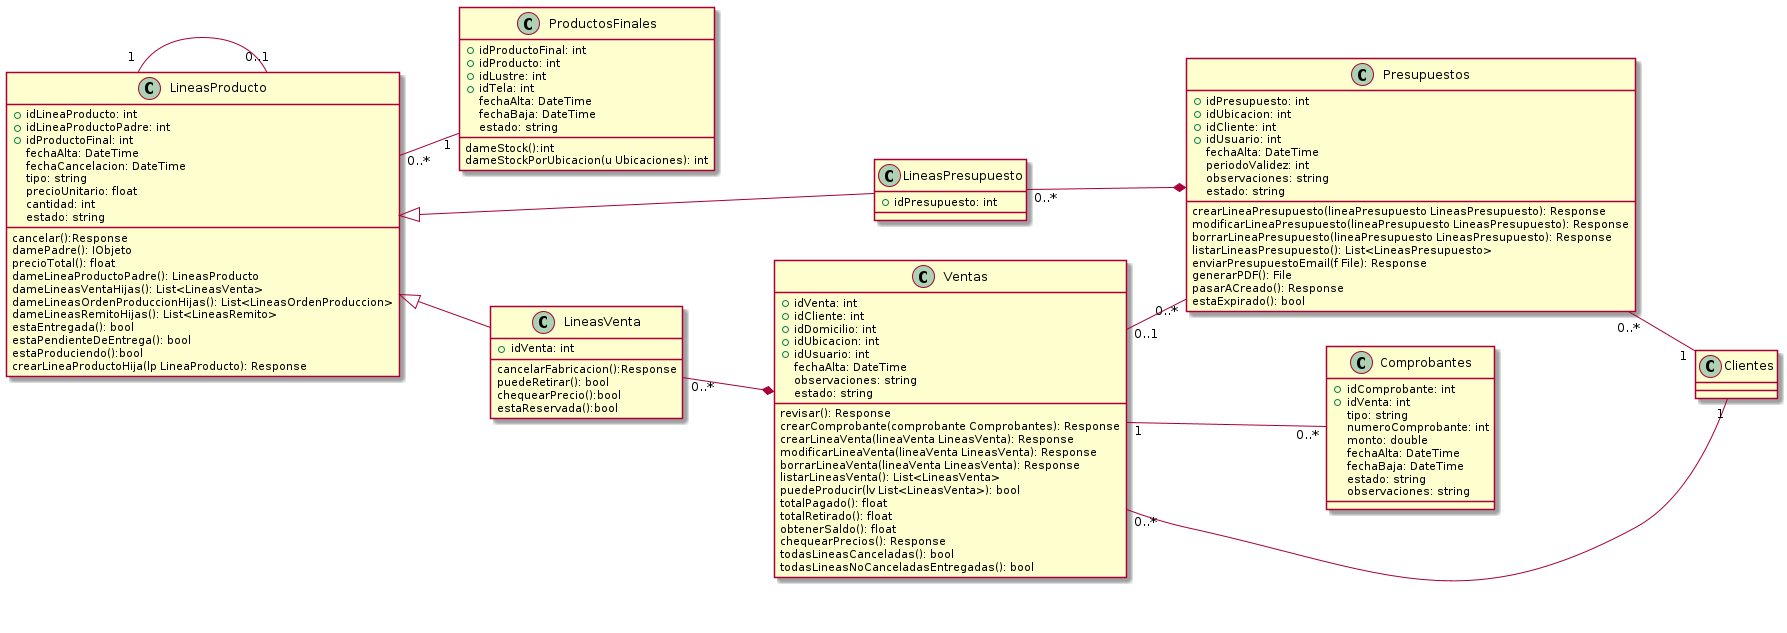
\includegraphics[width=\textwidth,height=0.90\textheight,keepaspectratio]{DiagramaClases/Vistas/vistaPresupuestosVentas}
		\caption{Diagrama de clases - Vista presupuestos y ventas}
	\label{fig:Diagrama de clases - Vista presupuestos y ventas}
	\end{figure}

	\begin{figure}[H]
		\centering
		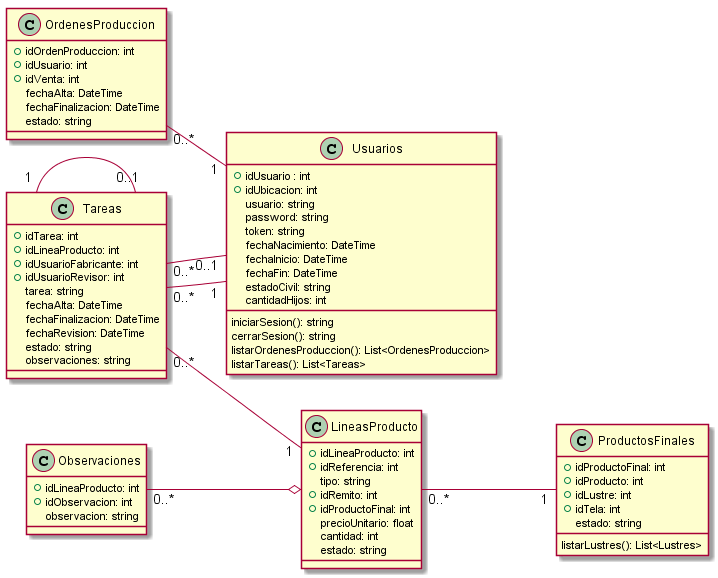
\includegraphics[width=\textwidth,height=0.90\textheight,keepaspectratio]{DiagramaClases/Vistas/vistaProduccion}
		\caption{Diagrama de clases - Vista producción}
	\label{fig:Diagrama de clases - Vista producción}
	\end{figure}

	\begin{figure}[H]
		\centering
		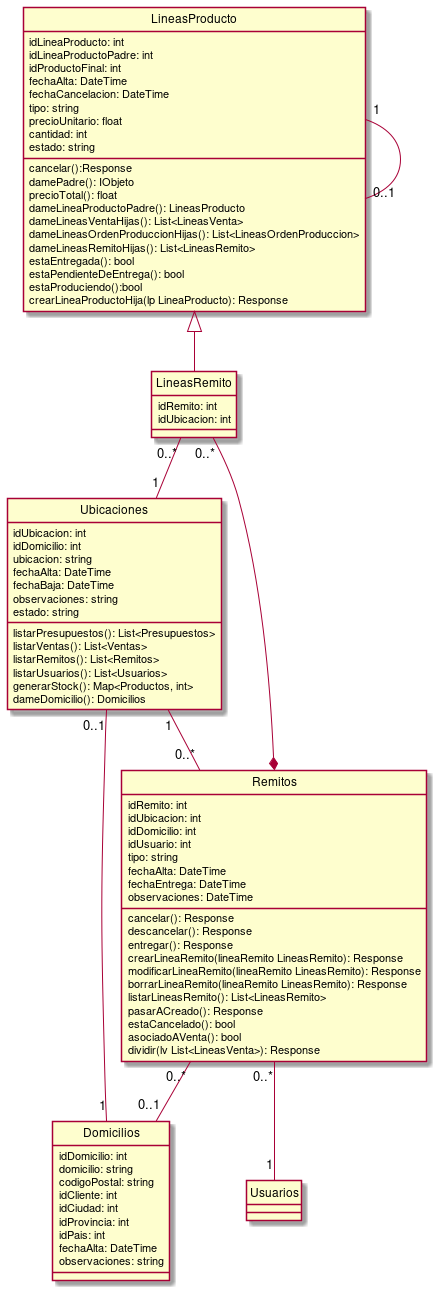
\includegraphics[width=\textwidth,height=0.5\textheight,keepaspectratio]{DiagramaClases/Vistas/vistaEntregas}
		\caption{Diagrama de clases - Vista entregas}
	\label{fig:Diagrama de clases - Vista entregas}
	\end{figure}

	\subsection{Vista canónica}
	\begin{figure}[H]
		\centering
		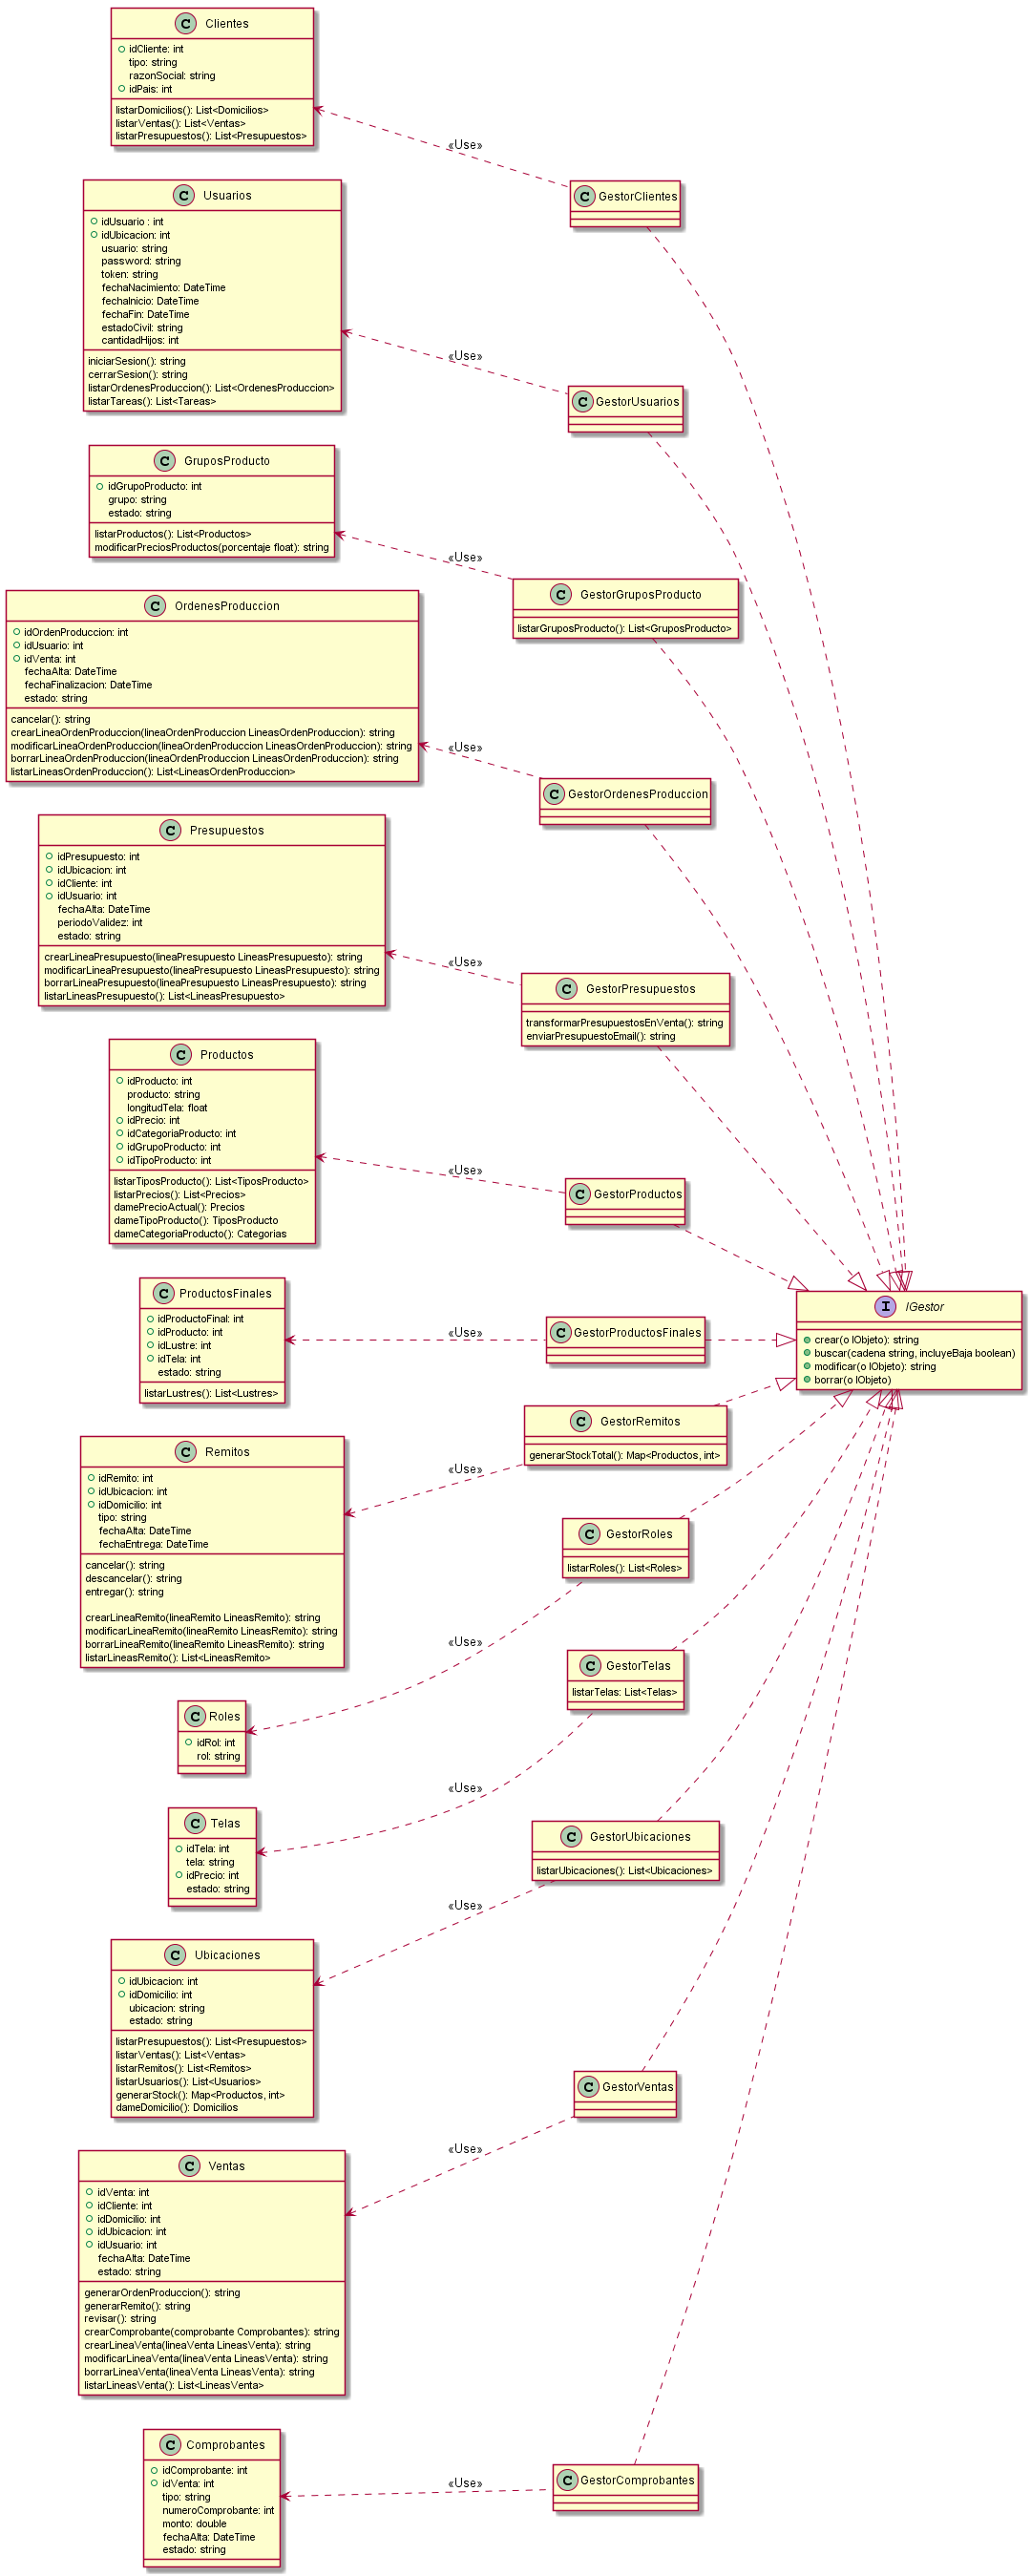
\includegraphics[width=\textwidth,height=0.9\textheight,keepaspectratio]{DiagramaClases/Vistas/vistaCanonica}
		\caption{Diagrama de clases - Vista canónica}
	\label{fig:Modelo de clases - Vista canónica}
	\end{figure}

	\subsection{Ficha técnica de clases}
	\begin{figure}[H]
		\centering
		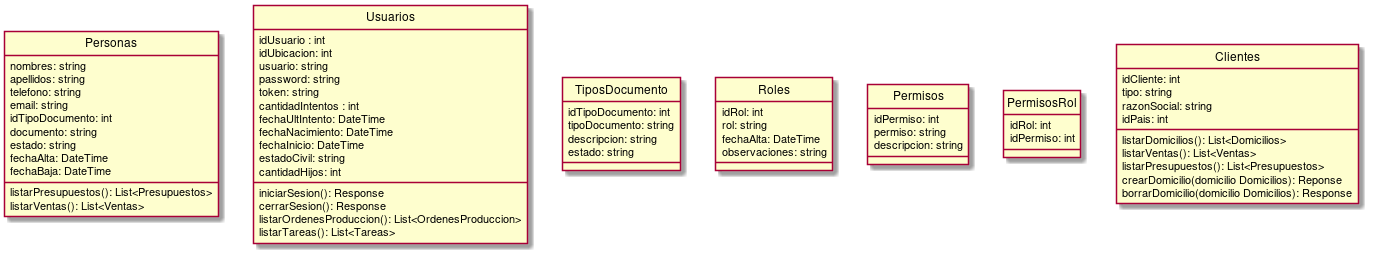
\includegraphics[width=\textwidth,height=0.9\textheight,keepaspectratio]{DiagramaClases/Vistas/fichaTecnicaClases1}
		\caption{Diagrama de clases - Ficha técnica de clases (Parte 1)}
	\label{fig:Modelo de clases - Ficha técnica de clases 1}
	\end{figure}
	\begin{figure}[H]
		\centering
		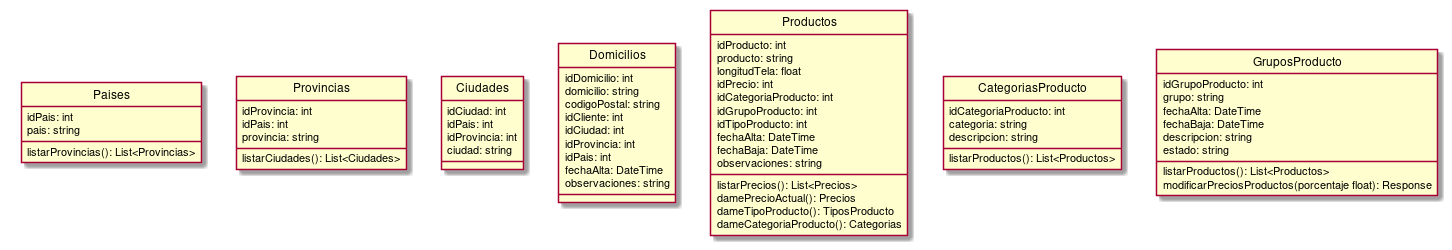
\includegraphics[width=\textwidth,height=0.9\textheight,keepaspectratio]{DiagramaClases/Vistas/fichaTecnicaClases2}
		\caption{Diagrama de clases - Ficha técnica de clases (Parte 2)}
	\label{fig:Modelo de clases - Ficha técnica de clases 2}
	\end{figure}
	\begin{figure}[H]
		\centering
		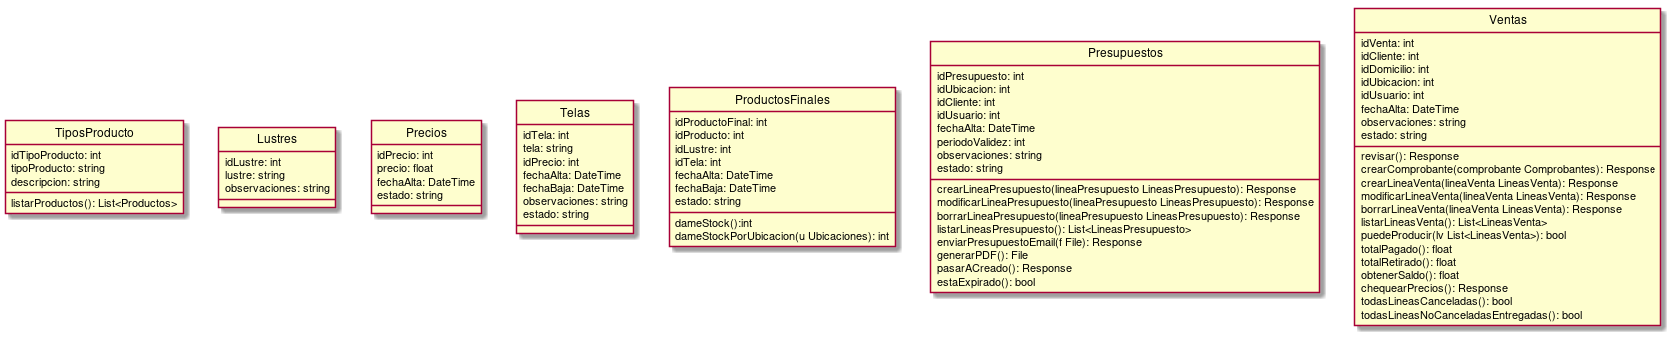
\includegraphics[width=\textwidth,height=0.9\textheight,keepaspectratio]{DiagramaClases/Vistas/fichaTecnicaClases3}
		\caption{Diagrama de clases - Ficha técnica de clases (Parte 3)}
	\label{fig:Modelo de clases - Ficha técnica de clases 3}
	\end{figure}
	\begin{figure}[H]
		\centering
		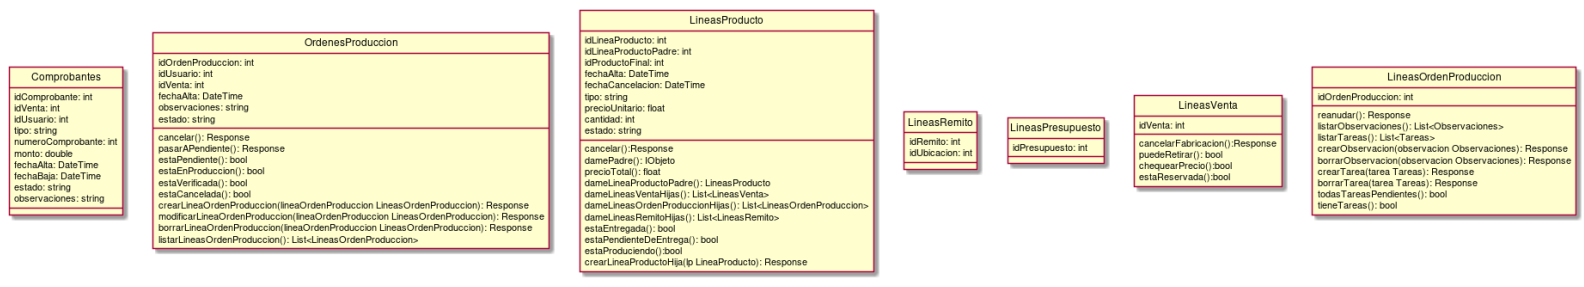
\includegraphics[width=\textwidth,height=0.9\textheight,keepaspectratio]{DiagramaClases/Vistas/fichaTecnicaClases4}
		\caption{Diagrama de clases - Ficha técnica de clases (Parte 4)}
	\label{fig:Modelo de clases - Ficha técnica de clases 4}
	\end{figure}
	\begin{figure}[H]
		\centering
		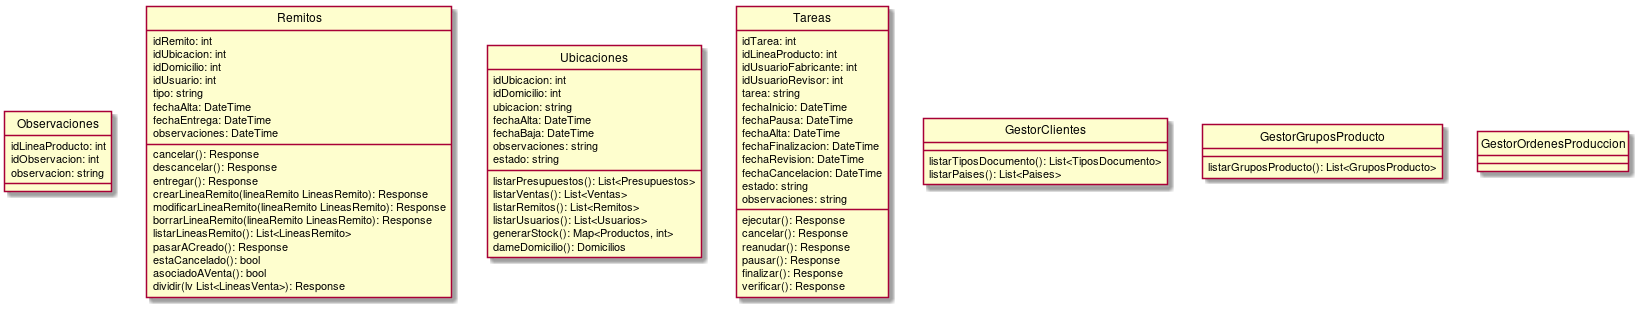
\includegraphics[width=\textwidth,height=0.9\textheight,keepaspectratio]{DiagramaClases/Vistas/fichaTecnicaClases5}
		\caption{Diagrama de clases - Ficha técnica de clases (Parte 5)}
	\label{fig:Modelo de clases - Ficha técnica de clases 5}
	\end{figure}
	\begin{figure}[H]
		\centering
		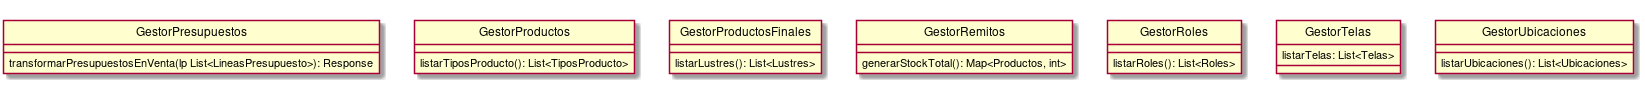
\includegraphics[width=\textwidth,height=0.9\textheight,keepaspectratio]{DiagramaClases/Vistas/fichaTecnicaClases6}
		\caption{Diagrama de clases - Ficha técnica de clases (Parte 6)}
	\label{fig:Modelo de clases - Ficha técnica de clases 6}
	\end{figure}
	\begin{figure}[H]
		\centering
		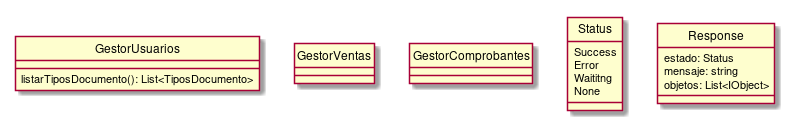
\includegraphics[width=\textwidth,height=0.9\textheight,keepaspectratio]{DiagramaClases/Vistas/fichaTecnicaClases7}
		\caption{Diagrama de clases - Ficha técnica de clases (Parte 7)}
	\label{fig:Modelo de clases - Ficha técnica de clases 7}
	\end{figure}

	\subsection{Diagramas de transición de estados}
	Solo se especificarán los diagramas de transición de estados más relevantes del sistema.
	\begin{figure}[H]
		\centering
		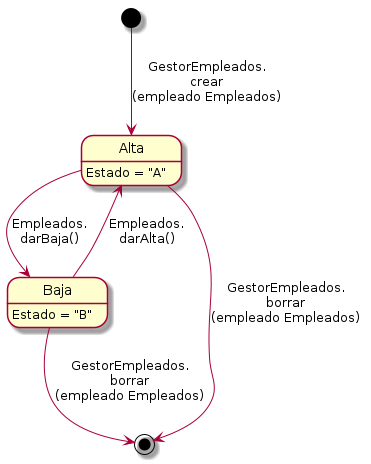
\includegraphics[width=0.6\textwidth,height=0.5\textheight,keepaspectratio]{DiagramasEstado/DiagramaDeEstado/empleados}
		\caption{Diagrama de transición de estados - Empleados}
		\label{fig:Diagrama de transición de estados - Empleados}
	\end{figure}
	\begin{figure}[H]
		\centering
		\includegraphics[width=\textwidth,height=\textheight,keepaspectratio]{DiagramasEstado/DiagramaDeEstado/tareas}
		\caption{Diagrama de transición de estados - Tareas}
		\label{fig:Diagrama de transición de estados - Tareas}
	\end{figure}
	\begin{figure}[H]
		\centering
		\includegraphics[width=\textwidth,height=\textheight,keepaspectratio]{DiagramasEstado/DiagramaDeEstado/lineasProducto}
		\caption{Diagrama de transición de estados - Líneas de producto}
		\label{fig:Diagrama de transición de estados - Líneas de producto}
	\end{figure}
	\begin{figure}[H]
		\centering
		\includegraphics[width=\textwidth,height=\textheight,keepaspectratio]{DiagramasEstado/DiagramaDeEstado/presupuestos}
		\caption{Diagrama de transición de estados - Presupuestos}
		\label{fig:Diagrama de transición de estados - Presupuestos}
	\end{figure}
	\begin{figure}[H]
		\centering
		\includegraphics[width=\textwidth,height=\textheight,keepaspectratio]{DiagramasEstado/DiagramaDeEstado/ventas}
		\caption{Diagrama de transición de estados - Ventas}
		\label{fig:Diagrama de transición de estados - Ventas}
	\end{figure}
	\begin{figure}[H]
		\centering
		\includegraphics[width=\textwidth,height=\textheight,keepaspectratio]{DiagramasEstado/DiagramaDeEstado/ordenesProduccion}
		\caption{Diagrama de transición de estados - Órdenes de producción}
		\label{fig:Diagrama de transición de estados - Órdenes de producción}
	\end{figure}
	\begin{figure}[H]
		\centering
		\includegraphics[width=\textwidth,height=\textheight,keepaspectratio]{DiagramasEstado/DiagramaDeEstado/remitos}
		\caption{Diagrama de transición de estados - Remitos}
		\label{fig:Diagrama de transición de estados - Remitos}
	\end{figure}

	\clearpage %salto de pagina
	\subsection{Diagramas de secuencia}
	Sólo se necesitaron los siguientes diagramas de secuencia para inferir las operaciones de las clases que permiten el comportamiento emergente de los casos de uso:

	\begin{figure}[H]
		\centering
		\includegraphics[width=\textwidth,height=\textheight,keepaspectratio]{DiagramasSecuencia/DiagramaDeSecuencia/GestionUsuarios}
		\caption{Diagrama de secuencia - Gestión de usuarios}
		\label{fig:Diagrama de secuencia - Gestión de usuarios}
	\end{figure}

	\begin{figure}[H]
		\centering
		\includegraphics[width=\textwidth,height=\textheight,keepaspectratio]{DiagramasSecuencia/DiagramaDeSecuencia/GestionClientes}
		\caption{Diagrama de secuencia - Gestión de clientes}
		\label{fig:Diagrama de secuencia - Gestión de clientes}
	\end{figure}

	\begin{figure}[H]
		\centering
		\includegraphics[width=\textwidth,height=\textheight,keepaspectratio]{DiagramasSecuencia/DiagramaDeSecuencia/GestionPresupuestos}
		\caption{Diagrama de secuencia - Gestión de presupuestos}
		\label{fig:Diagrama de secuencia - Gestión de presupuestos}
	\end{figure}

	\begin{figure}[H]
		\centering
		\includegraphics[width=\textwidth,height=\textheight,keepaspectratio]{DiagramasSecuencia/DiagramaDeSecuencia/GestionVentas}
		\caption{Diagrama de secuencia - Gestión de ventas}
		\label{fig:Diagrama de secuencia - Gestión de ventas}
	\end{figure}

	\clearpage %salto de pagina
	
	
		
	
    
\section{Identificación de roles, sus funciones y restricciones:}
    \subsection{Roles}
    Los usuarios finales en el sistema pueden cumplir uno de los siguientes roles:
    \begin{itemize}
        \item Administrador.
        \item Vendedor.
        \item Fabricante.
    \end{itemize}
    
    \subsection{Funciones de los usuarios por rol}
    \begin{itemize}
        \item Rol administrador:
        \begin{itemize}
            \item Sesiones
            \begin{itemize}
                \item Iniciar sesión
                \item Cerrar sesión
            \end{itemize}
            \item Gestión empleados
            \begin{itemize}
                \item Crear empleado
                \item Buscar avanzado empleados
                \item Dar de baja empleado
                \item Dar de alta empleado
                \item Modificar empleado
                \item Borrar empleado
            \end{itemize}
            \item Gestión roles
            \begin{itemize}
                \item Crear rol
                \item Listar roles
                \item Modificar rol
                \item Borrar rol
            \end{itemize}
            \item Gestión productos
            \begin{itemize}
                \item Crear producto
                \item Buscar avanzado productos
                \item Dar de baja producto
                \item Dar de alta producto
                \item Modificar producto
                \item Borrar producto
            \end{itemize}
            \item Gestión telas
            \begin{itemize}
                \item Crear tela
                \item Listar telas
                \item Dar de baja tela
                \item Dar de alta tela
                \item Modificar tela
                \item Borrar tela
            \end{itemize}
            \item Gestión productos finales
            \begin{itemize}
                \item Crear producto final
                \item Buscar avanzado productos finales
                \item Dar de baja producto final
                \item Dar de alta producto final
                \item Modificar producto final
                \item Borrar producto final
            \end{itemize}
            \item Gestión grupos de producto
            \begin{itemize}
                \item Crear grupo de producto
                \item Listar grupos de producto
                \item Dar de baja grupo de producto
                \item Dar de alta grupo de producto
                \item Modificar grupo de producto
                \item Borrar grupo de producto
                \item Listar productos por grupo
                \item Modificar precios de producto por grupo
            \end{itemize}
            \item Gestión ubicaciones
            \begin{itemize}
                \item Crear ubicación
                \item Listar ubicaciones
                \item Dar de baja ubicación
                \item Dar de alta ubicación
                \item Modificar ubicación
                \item Borrar ubicación
            \end{itemize}
            \item Gestión remitos
            \begin{itemize}
                \item Crear remito
                \item Buscar avanzado remitos
                \item Cancelar remito
                \item Descancelar remito
                \item Entregar remito
                \item Borrar remito
                \item Listar líneas de remito
            \end{itemize}
            \item Gestión líneas de remito
            \begin{itemize}
                \item Crear línea remito
                \item Modificar línea de remito
                \item Borrar línea de remito
            \end{itemize}
            \item Gestión clientes
            \begin{itemize}
                \item Crear cliente
                \item Buscar avanzado clientes
                \item Dar de baja cliente
                \item Dar de alta cliente
                \item Modificar cliente
                \item Borrar cliente
            \end{itemize}
            \item Gestión presupuestos
            \begin{itemize}
                \item Crear presupuesto
                \item Buscar avanzado presupuestos
                \item Modificar presupuesto
                \item Borrar presupuesto
                \item Transformar presupuesto en venta
                \item Generar presupuesto en formato PDF
                \item Enviar presupuesto por correo electrónico
                \item Listar líneas de presupuesto
            \end{itemize}
            \item Gestión líneas de presupuesto
            \begin{itemize}
                \item Crear línea de presupuesto
                \item Modificar línea de presupuesto
                \item Borrar línea de presupuesto
            \end{itemize}
            \item Gestión ventas
            \begin{itemize}
                \item Crear venta
                \item Buscar avanzado ventas
                \item Listar líneas de venta
                \item Modificar venta
                \item Borrar venta
                \item Generar orden de producción a partir de venta
                \item Generar remito a partir de venta
                \item Crear comprobante 
                \item Revisar venta
            \end{itemize}
            \item Gestión líneas de venta
            \begin{itemize}
                \item Crear línea de venta
                \item Modificar línea de venta
                \item Borrar línea de venta
                \item Cancelar línea de venta
            \end{itemize}
            \item Gestión comprobantes
            \begin{itemize}
                \item Buscar avanzado comprobantes
                \item Modificar comprobante
                \item Borrar comprobante
            \end{itemize}
            \item Gestión órdenes de producción
            \begin{itemize}
                \item Crear orden de producción
                \item Buscar avanzado órdenes de producción
                \item Modificar orden de producción
                \item Listar lineas de orden de producción
                \item Borrar orden de producción
                \item Cancelar orden de producción
                \item Listar observaciones de línea de orden de producción
                \item Listar tareas de línea de orden de producción
            \end{itemize}
            \item Gestión líneas de órdenes de producción
            \begin{itemize}
                \item Crear línea de orden de producción
                \item Modificar línea de orden de producción
                \item Borrar línea de orden de producción
                \item Verificar línea de orden de producción
                \item Cancelar línea de orden de producción	
                \item Reanudar línea de orden de producción		
            \end{itemize}
            \item Gestión observaciones
            \begin{itemize}
                \item Crear observación
                \item Borrar observación
            \end{itemize}
            \item Gestión tareas
            \begin{itemize}
                \item Crear tarea
                \item Borrar tarea
                \item Finalizar tarea
                \item Verificar tarea
                \item Pausar tarea
                \item Reanudar tarea
                \item Cancelar tarea
                \item Ejecutar tarea
            \end{itemize}
        \end{itemize}
        
        \item Rol vendedor:
        \begin{itemize}
            \item Sesiones
            \begin{itemize}
                \item Iniciar sesión
                \item Cerrar sesión
            \end{itemize}
            \item Gestión productos
            \begin{itemize}
                \item Buscar avanzado productos
            \end{itemize}
            \item Gestión telas
            \begin{itemize}
                \item Listar telas
            \end{itemize}
            \item Gestión productos finales
            \begin{itemize}
                \item Crear producto final
                \item Buscar avanzado productos finales
            \end{itemize}
            \item Gestión ubicaciones
            \begin{itemize}
                \item Listar ubicaciones
            \end{itemize}
            \item Gestión remitos
            \begin{itemize}
                \item Crear remito
                \item Buscar avanzado remitos
                \item Entregar remito
                \item Listar líneas de remito
            \end{itemize}
            \item Gestión líneas de remito
            \begin{itemize}
                \item Crear línea remito
                \item Modificar línea de remito
            \end{itemize}
            \item Gestión clientes
            \begin{itemize}
                \item Crear cliente
                \item Buscar avanzado clientes
                \item Modificar cliente
                \item Borrar cliente
            \end{itemize}
            \item Gestión presupuestos
            \begin{itemize}
                \item Crear presupuesto
                \item Buscar avanzado presupuestos
                \item Modificar presupuesto
                \item Transformar presupuesto en venta
                \item Generar presupuesto en formato PDF
                \item Enviar presupuesto por correo electrónico
                \item Listar líneas de presupuesto
            \end{itemize}
            \item Gestión líneas de presupuesto
            \begin{itemize}
                \item Crear línea de presupuesto
                \item Modificar línea de presupuesto
                \item Borrar línea de presupuesto
            \end{itemize}
            \item Gestión ventas
            \begin{itemize}
                \item Crear venta
                \item Buscar avanzado ventas
                \item Listar líneas de venta
                \item Modificar venta
                \item Generar remito a partir de venta
                \item Crear comprobante
            \end{itemize}
            \item Gestión líneas de venta
            \begin{itemize}
                \item Crear línea de venta
                \item Modificar línea de venta
                \item Borrar línea de venta
            \end{itemize}
            \item Gestión comprobantes
            \begin{itemize}
                \item Buscar avanzado comprobantes
            \end{itemize}
        \end{itemize}
        
        \item Rol fabricante:
        \begin{itemize}
            \item Sesiones
            \begin{itemize}
                \item Iniciar sesión
                \item Cerrar sesión
            \end{itemize}
            \item Gestión órdenes de producción
            \begin{itemize}
                \item Buscar avanzado órdenes de producción
                \item Listar lineas de orden de producción
                \item Listar observaciones de línea de orden de producción
                \item Listar tareas de línea de orden de producción
            \end{itemize}
            \item Gestión tareas
            \begin{itemize}
                \item Finalizar tarea
                \item Ejecutar tarea
            \end{itemize}
        \end{itemize}
    \end{itemize}
    \subsection{Restricciones de datos}
    Todos los roles tendrán restricción para insertar, modificar, borrar y leer cualquier tabla. Las consultas se realizarán a través de los Stored Procedures.
%\section{Identificación de roles, sus funciones y restricciones:}
    \subsection{Roles}
    Los usuarios finales en el sistema pueden cumplir uno de los siguientes roles:
    \begin{itemize}
        \item Administrador.
        \item Vendedor.
        \item Fabricante.
    \end{itemize}
    
    \subsection{Funciones de los usuarios por rol}
    \begin{itemize}
        \item Rol administrador:
        \begin{itemize}
            \item Sesiones
            \begin{itemize}
                \item Iniciar sesión
                \item Cerrar sesión
            \end{itemize}
            \item Gestión empleados
            \begin{itemize}
                \item Crear empleado
                \item Buscar avanzado empleados
                \item Dar de baja empleado
                \item Dar de alta empleado
                \item Modificar empleado
                \item Borrar empleado
            \end{itemize}
            \item Gestión roles
            \begin{itemize}
                \item Crear rol
                \item Listar roles
                \item Modificar rol
                \item Borrar rol
            \end{itemize}
            \item Gestión productos
            \begin{itemize}
                \item Crear producto
                \item Buscar avanzado productos
                \item Dar de baja producto
                \item Dar de alta producto
                \item Modificar producto
                \item Borrar producto
            \end{itemize}
            \item Gestión telas
            \begin{itemize}
                \item Crear tela
                \item Listar telas
                \item Dar de baja tela
                \item Dar de alta tela
                \item Modificar tela
                \item Borrar tela
            \end{itemize}
            \item Gestión productos finales
            \begin{itemize}
                \item Crear producto final
                \item Buscar avanzado productos finales
                \item Dar de baja producto final
                \item Dar de alta producto final
                \item Modificar producto final
                \item Borrar producto final
            \end{itemize}
            \item Gestión grupos de producto
            \begin{itemize}
                \item Crear grupo de producto
                \item Listar grupos de producto
                \item Dar de baja grupo de producto
                \item Dar de alta grupo de producto
                \item Modificar grupo de producto
                \item Borrar grupo de producto
                \item Listar productos por grupo
                \item Modificar precios de producto por grupo
            \end{itemize}
            \item Gestión ubicaciones
            \begin{itemize}
                \item Crear ubicación
                \item Listar ubicaciones
                \item Dar de baja ubicación
                \item Dar de alta ubicación
                \item Modificar ubicación
                \item Borrar ubicación
            \end{itemize}
            \item Gestión remitos
            \begin{itemize}
                \item Crear remito
                \item Buscar avanzado remitos
                \item Cancelar remito
                \item Descancelar remito
                \item Entregar remito
                \item Borrar remito
                \item Listar líneas de remito
            \end{itemize}
            \item Gestión líneas de remito
            \begin{itemize}
                \item Crear línea remito
                \item Modificar línea de remito
                \item Borrar línea de remito
            \end{itemize}
            \item Gestión clientes
            \begin{itemize}
                \item Crear cliente
                \item Buscar avanzado clientes
                \item Dar de baja cliente
                \item Dar de alta cliente
                \item Modificar cliente
                \item Borrar cliente
            \end{itemize}
            \item Gestión presupuestos
            \begin{itemize}
                \item Crear presupuesto
                \item Buscar avanzado presupuestos
                \item Modificar presupuesto
                \item Borrar presupuesto
                \item Transformar presupuesto en venta
                \item Generar presupuesto en formato PDF
                \item Enviar presupuesto por correo electrónico
                \item Listar líneas de presupuesto
            \end{itemize}
            \item Gestión líneas de presupuesto
            \begin{itemize}
                \item Crear línea de presupuesto
                \item Modificar línea de presupuesto
                \item Borrar línea de presupuesto
            \end{itemize}
            \item Gestión ventas
            \begin{itemize}
                \item Crear venta
                \item Buscar avanzado ventas
                \item Listar líneas de venta
                \item Modificar venta
                \item Borrar venta
                \item Generar orden de producción a partir de venta
                \item Generar remito a partir de venta
                \item Crear comprobante 
                \item Revisar venta
            \end{itemize}
            \item Gestión líneas de venta
            \begin{itemize}
                \item Crear línea de venta
                \item Modificar línea de venta
                \item Borrar línea de venta
                \item Cancelar línea de venta
            \end{itemize}
            \item Gestión comprobantes
            \begin{itemize}
                \item Buscar avanzado comprobantes
                \item Modificar comprobante
                \item Borrar comprobante
            \end{itemize}
            \item Gestión órdenes de producción
            \begin{itemize}
                \item Crear orden de producción
                \item Buscar avanzado órdenes de producción
                \item Modificar orden de producción
                \item Listar lineas de orden de producción
                \item Borrar orden de producción
                \item Cancelar orden de producción
                \item Listar observaciones de línea de orden de producción
                \item Listar tareas de línea de orden de producción
            \end{itemize}
            \item Gestión líneas de órdenes de producción
            \begin{itemize}
                \item Crear línea de orden de producción
                \item Modificar línea de orden de producción
                \item Borrar línea de orden de producción
                \item Verificar línea de orden de producción
                \item Cancelar línea de orden de producción	
                \item Reanudar línea de orden de producción		
            \end{itemize}
            \item Gestión observaciones
            \begin{itemize}
                \item Crear observación
                \item Borrar observación
            \end{itemize}
            \item Gestión tareas
            \begin{itemize}
                \item Crear tarea
                \item Borrar tarea
                \item Finalizar tarea
                \item Verificar tarea
                \item Pausar tarea
                \item Reanudar tarea
                \item Cancelar tarea
                \item Ejecutar tarea
            \end{itemize}
        \end{itemize}
        
        \item Rol vendedor:
        \begin{itemize}
            \item Sesiones
            \begin{itemize}
                \item Iniciar sesión
                \item Cerrar sesión
            \end{itemize}
            \item Gestión productos
            \begin{itemize}
                \item Buscar avanzado productos
            \end{itemize}
            \item Gestión telas
            \begin{itemize}
                \item Listar telas
            \end{itemize}
            \item Gestión productos finales
            \begin{itemize}
                \item Crear producto final
                \item Buscar avanzado productos finales
            \end{itemize}
            \item Gestión ubicaciones
            \begin{itemize}
                \item Listar ubicaciones
            \end{itemize}
            \item Gestión remitos
            \begin{itemize}
                \item Crear remito
                \item Buscar avanzado remitos
                \item Entregar remito
                \item Listar líneas de remito
            \end{itemize}
            \item Gestión líneas de remito
            \begin{itemize}
                \item Crear línea remito
                \item Modificar línea de remito
            \end{itemize}
            \item Gestión clientes
            \begin{itemize}
                \item Crear cliente
                \item Buscar avanzado clientes
                \item Modificar cliente
                \item Borrar cliente
            \end{itemize}
            \item Gestión presupuestos
            \begin{itemize}
                \item Crear presupuesto
                \item Buscar avanzado presupuestos
                \item Modificar presupuesto
                \item Transformar presupuesto en venta
                \item Generar presupuesto en formato PDF
                \item Enviar presupuesto por correo electrónico
                \item Listar líneas de presupuesto
            \end{itemize}
            \item Gestión líneas de presupuesto
            \begin{itemize}
                \item Crear línea de presupuesto
                \item Modificar línea de presupuesto
                \item Borrar línea de presupuesto
            \end{itemize}
            \item Gestión ventas
            \begin{itemize}
                \item Crear venta
                \item Buscar avanzado ventas
                \item Listar líneas de venta
                \item Modificar venta
                \item Generar remito a partir de venta
                \item Crear comprobante
            \end{itemize}
            \item Gestión líneas de venta
            \begin{itemize}
                \item Crear línea de venta
                \item Modificar línea de venta
                \item Borrar línea de venta
            \end{itemize}
            \item Gestión comprobantes
            \begin{itemize}
                \item Buscar avanzado comprobantes
            \end{itemize}
        \end{itemize}
        
        \item Rol fabricante:
        \begin{itemize}
            \item Sesiones
            \begin{itemize}
                \item Iniciar sesión
                \item Cerrar sesión
            \end{itemize}
            \item Gestión órdenes de producción
            \begin{itemize}
                \item Buscar avanzado órdenes de producción
                \item Listar lineas de orden de producción
                \item Listar observaciones de línea de orden de producción
                \item Listar tareas de línea de orden de producción
            \end{itemize}
            \item Gestión tareas
            \begin{itemize}
                \item Finalizar tarea
                \item Ejecutar tarea
            \end{itemize}
        \end{itemize}
    \end{itemize}
    \subsection{Restricciones de datos}
    Todos los roles tendrán restricción para insertar, modificar, borrar y leer cualquier tabla. Las consultas se realizarán a través de los Stored Procedures.
\chapter{Especificación D}
\label{ch:capitulo5} 
\markboth{CAPÍTULO \ref*{ch:capitulo5}. Especificación D}{CAPÍTULO \ref*{ch:capitulo5}. Especificación D}
\section{Diseño del modelo lógico y físico de datos del sistema}
    \subsection{Modelo relacional}
        \begin{figure}[H]
            \centering
            \includegraphics[width=\textwidth,height=\textheight,keepaspectratio]{ModeloRelacional/modeloRelacional}
            \caption{Modelo relacional}
        \label{fig:Modelo relacional}
        \end{figure}
        \clearpage %salto de pagina
        \begin{figure}[H]
            \centering
            \includegraphics[width=\textwidth,height=0.90\textheight,keepaspectratio]{ModeloRelacional/vistaSistema}
            \caption{Modelo relacional - Vista sistema}
        \label{fig:Modelo relacional - Vista sistema}
        \end{figure}
        \begin{figure}[H]
            \centering
            \includegraphics[width=\textwidth,height=0.90\textheight,keepaspectratio]{ModeloRelacional/vistaClientes}
            \caption{Modelo relacional - Vista clientes}
        \label{fig:Modelo relacional - Vista clientes}
        \end{figure}
        \begin{figure}[H]
            \centering
            \includegraphics[width=\textwidth,height=0.90\textheight,keepaspectratio]{ModeloRelacional/vistaProductos}
            \caption{Modelo relacional - Vista productos}
        \label{fig:Modelo relacional - Vista productos}
        \end{figure}
        \begin{figure}[H]
            \centering
            \includegraphics[width=\textwidth,height=0.90\textheight,keepaspectratio]{ModeloRelacional/vistaPresupuestosVentas}
            \caption{Modelo relacional - Vista presupuestos y ventas}
        \label{fig:Modelo relacional - Vista presupuestos y ventas}
        \end{figure}
        \begin{figure}[H]
            \centering
            \includegraphics[width=\textwidth,height=0.90\textheight,keepaspectratio]{ModeloRelacional/vistaProduccion}
            \caption{Modelo relacional - Vista producción}
        \label{fig:Modelo relacional - Vista producción}
        \end{figure}

        \begin{figure}[H]
            \centering
            \includegraphics[width=0.7\textwidth,height=0.5\textheight,keepaspectratio]{ModeloRelacional/vistaEntregas}
            \caption{Modelo relacional - Vista entregas}
        \label{fig:Modelo relacional - Vista entregas}
        \end{figure}
\section{Arquitectura física del sistema}
\paragraph\indent
\textbf{Arquitectura del sistema:} Es la tecnología que proporciona al usuario final el acceso transparente a las aplicaciones, datos, servicios de cómputo o cualquier otro recurso a través de la organización en múltiples plataformas. El modelo soporta un medio ambiente distribuido en el cual los requerimientos de servicio hechos por estaciones de trabajo inteligentes o clientes resultan en un trabajo realizado por otros computadores llamados servidores.

\textbf{Cliente:} Es el que inicia un requerimiento de servicio. El requerimiento inicial puede convertirse en múltiples requerimientos de trabajo. La ubicación de los datos o de las aplicaciones es totalmente transparente para el cliente.

\textbf{Servidor:} Es cualquier recurso de cómputo dedicado a responder a los requerimientos del cliente. Los servidores pueden estar conectados a los clientes a través de redes LAN o WAN para proveer de múltiples servicios a los clientes tales como impresión, acceso a bases de datos, fax, procesamiento de imágenes, etc.
\paragraph\indent
La arquitectura cliente-servidor es un modelo de aplicación distribuida en el que las tareas se reparten entre los servidores, que proveen de recursos o servicios, y los clientes, que demandan por estos recursos y servicios. Si un cliente realiza peticiones a otro programa es el servidor quien le da una respuesta.

\subsection{Ventajas}
\begin{itemize}
	\item Centralización del control: los accesos, recursos y la integridad de los datos son controlados por el servidor de forma que un programa cliente defectuoso o no autorizado no pueda dañar el sistema. Esta centralización también facilita la tarea de poner al día datos u otros recursos.
	\item Escalabilidad: se puede aumentar la capacidad de clientes y servidores por separado. Cualquier elemento puede ser mejorado en cualquier momento, o se pueden añadir nuevos nodos a la red (clientes y/o servidores).
	\item Fácil mantenimiento: al estar distribuidas las funciones y responsabilidades entre varios ordenadores independientes, es posible reemplazar, reparar, actualizar, o incluso trasladar un servidor, mientras que sus clientes no se verán afectados por ese cambio. Esta independencia de los cambios también se conoce como encapsulación.
	\item Tecnologías: Existen tecnologías, suficientemente desarrolladas, diseñadas para el paradigma de C/S que aseguran la seguridad en las transacciones, la amigabilidad de la interfaz, y la facilidad de empleo.
\end{itemize}

\subsection{Desventajas}
\begin{itemize}
	\item Tráfico: La congestión del tráfico ha sido siempre un problema en el paradigma de C/S. Cuando una gran cantidad de clientes envían peticiones simultáneas al mismo servidor, puede ser que cause muchos problemas para éste.
	\item Robustez: El paradigma de C/S clásico no tiene la robustez de una red P2P. Cuando un servidor está caído, las peticiones de los clientes no pueden ser satisfechas.
	\item El software y el hardware de un servidor son generalmente muy determinantes. Un hardware regular de un ordenador personal puede no poder servir a cierta cantidad de clientes. Normalmente se necesita software y hardware específico, sobre todo en el lado del servidor, para satisfacer el trabajo.
	\item El cliente no dispone de los recursos que puedan existir en el servidor. Por ejemplo, si la aplicación es una Web, no podemos escribir en el disco duro del cliente o imprimir directamente sobre las impresoras sin sacar antes la ventana previa de impresión de los navegadores.
\end{itemize}

\section{Diagrama de despliegue}
Un diagrama de despliegue modela la arquitectura en tiempo de ejecución de un sistema. Esto muestra la configuración de los elementos de hardware y muestra cómo los elementos y artefactos del software se trazan en esos nodos.
\begin{figure}[H]
		\centering
		\includegraphics[width=\textwidth,height=0.95\textheight,keepaspectratio]{Extras/diagramaDespliegue}
		\caption{Diagrama de despliegue}
	\label{fig:diagramaDespliegue}
	\end{figure}
%\section{Identificación de roles, sus funciones y restricciones:}
    \subsection{Roles}
    Los usuarios finales en el sistema pueden cumplir uno de los siguientes roles:
    \begin{itemize}
        \item Administrador.
        \item Vendedor.
        \item Fabricante.
    \end{itemize}
    
    \subsection{Funciones de los usuarios por rol}
    \begin{itemize}
        \item Rol administrador:
        \begin{itemize}
            \item Sesiones
            \begin{itemize}
                \item Iniciar sesión
                \item Cerrar sesión
            \end{itemize}
            \item Gestión empleados
            \begin{itemize}
                \item Crear empleado
                \item Buscar avanzado empleados
                \item Dar de baja empleado
                \item Dar de alta empleado
                \item Modificar empleado
                \item Borrar empleado
            \end{itemize}
            \item Gestión roles
            \begin{itemize}
                \item Crear rol
                \item Listar roles
                \item Modificar rol
                \item Borrar rol
            \end{itemize}
            \item Gestión productos
            \begin{itemize}
                \item Crear producto
                \item Buscar avanzado productos
                \item Dar de baja producto
                \item Dar de alta producto
                \item Modificar producto
                \item Borrar producto
            \end{itemize}
            \item Gestión telas
            \begin{itemize}
                \item Crear tela
                \item Listar telas
                \item Dar de baja tela
                \item Dar de alta tela
                \item Modificar tela
                \item Borrar tela
            \end{itemize}
            \item Gestión productos finales
            \begin{itemize}
                \item Crear producto final
                \item Buscar avanzado productos finales
                \item Dar de baja producto final
                \item Dar de alta producto final
                \item Modificar producto final
                \item Borrar producto final
            \end{itemize}
            \item Gestión grupos de producto
            \begin{itemize}
                \item Crear grupo de producto
                \item Listar grupos de producto
                \item Dar de baja grupo de producto
                \item Dar de alta grupo de producto
                \item Modificar grupo de producto
                \item Borrar grupo de producto
                \item Listar productos por grupo
                \item Modificar precios de producto por grupo
            \end{itemize}
            \item Gestión ubicaciones
            \begin{itemize}
                \item Crear ubicación
                \item Listar ubicaciones
                \item Dar de baja ubicación
                \item Dar de alta ubicación
                \item Modificar ubicación
                \item Borrar ubicación
            \end{itemize}
            \item Gestión remitos
            \begin{itemize}
                \item Crear remito
                \item Buscar avanzado remitos
                \item Cancelar remito
                \item Descancelar remito
                \item Entregar remito
                \item Borrar remito
                \item Listar líneas de remito
            \end{itemize}
            \item Gestión líneas de remito
            \begin{itemize}
                \item Crear línea remito
                \item Modificar línea de remito
                \item Borrar línea de remito
            \end{itemize}
            \item Gestión clientes
            \begin{itemize}
                \item Crear cliente
                \item Buscar avanzado clientes
                \item Dar de baja cliente
                \item Dar de alta cliente
                \item Modificar cliente
                \item Borrar cliente
            \end{itemize}
            \item Gestión presupuestos
            \begin{itemize}
                \item Crear presupuesto
                \item Buscar avanzado presupuestos
                \item Modificar presupuesto
                \item Borrar presupuesto
                \item Transformar presupuesto en venta
                \item Generar presupuesto en formato PDF
                \item Enviar presupuesto por correo electrónico
                \item Listar líneas de presupuesto
            \end{itemize}
            \item Gestión líneas de presupuesto
            \begin{itemize}
                \item Crear línea de presupuesto
                \item Modificar línea de presupuesto
                \item Borrar línea de presupuesto
            \end{itemize}
            \item Gestión ventas
            \begin{itemize}
                \item Crear venta
                \item Buscar avanzado ventas
                \item Listar líneas de venta
                \item Modificar venta
                \item Borrar venta
                \item Generar orden de producción a partir de venta
                \item Generar remito a partir de venta
                \item Crear comprobante 
                \item Revisar venta
            \end{itemize}
            \item Gestión líneas de venta
            \begin{itemize}
                \item Crear línea de venta
                \item Modificar línea de venta
                \item Borrar línea de venta
                \item Cancelar línea de venta
            \end{itemize}
            \item Gestión comprobantes
            \begin{itemize}
                \item Buscar avanzado comprobantes
                \item Modificar comprobante
                \item Borrar comprobante
            \end{itemize}
            \item Gestión órdenes de producción
            \begin{itemize}
                \item Crear orden de producción
                \item Buscar avanzado órdenes de producción
                \item Modificar orden de producción
                \item Listar lineas de orden de producción
                \item Borrar orden de producción
                \item Cancelar orden de producción
                \item Listar observaciones de línea de orden de producción
                \item Listar tareas de línea de orden de producción
            \end{itemize}
            \item Gestión líneas de órdenes de producción
            \begin{itemize}
                \item Crear línea de orden de producción
                \item Modificar línea de orden de producción
                \item Borrar línea de orden de producción
                \item Verificar línea de orden de producción
                \item Cancelar línea de orden de producción	
                \item Reanudar línea de orden de producción		
            \end{itemize}
            \item Gestión observaciones
            \begin{itemize}
                \item Crear observación
                \item Borrar observación
            \end{itemize}
            \item Gestión tareas
            \begin{itemize}
                \item Crear tarea
                \item Borrar tarea
                \item Finalizar tarea
                \item Verificar tarea
                \item Pausar tarea
                \item Reanudar tarea
                \item Cancelar tarea
                \item Ejecutar tarea
            \end{itemize}
        \end{itemize}
        
        \item Rol vendedor:
        \begin{itemize}
            \item Sesiones
            \begin{itemize}
                \item Iniciar sesión
                \item Cerrar sesión
            \end{itemize}
            \item Gestión productos
            \begin{itemize}
                \item Buscar avanzado productos
            \end{itemize}
            \item Gestión telas
            \begin{itemize}
                \item Listar telas
            \end{itemize}
            \item Gestión productos finales
            \begin{itemize}
                \item Crear producto final
                \item Buscar avanzado productos finales
            \end{itemize}
            \item Gestión ubicaciones
            \begin{itemize}
                \item Listar ubicaciones
            \end{itemize}
            \item Gestión remitos
            \begin{itemize}
                \item Crear remito
                \item Buscar avanzado remitos
                \item Entregar remito
                \item Listar líneas de remito
            \end{itemize}
            \item Gestión líneas de remito
            \begin{itemize}
                \item Crear línea remito
                \item Modificar línea de remito
            \end{itemize}
            \item Gestión clientes
            \begin{itemize}
                \item Crear cliente
                \item Buscar avanzado clientes
                \item Modificar cliente
                \item Borrar cliente
            \end{itemize}
            \item Gestión presupuestos
            \begin{itemize}
                \item Crear presupuesto
                \item Buscar avanzado presupuestos
                \item Modificar presupuesto
                \item Transformar presupuesto en venta
                \item Generar presupuesto en formato PDF
                \item Enviar presupuesto por correo electrónico
                \item Listar líneas de presupuesto
            \end{itemize}
            \item Gestión líneas de presupuesto
            \begin{itemize}
                \item Crear línea de presupuesto
                \item Modificar línea de presupuesto
                \item Borrar línea de presupuesto
            \end{itemize}
            \item Gestión ventas
            \begin{itemize}
                \item Crear venta
                \item Buscar avanzado ventas
                \item Listar líneas de venta
                \item Modificar venta
                \item Generar remito a partir de venta
                \item Crear comprobante
            \end{itemize}
            \item Gestión líneas de venta
            \begin{itemize}
                \item Crear línea de venta
                \item Modificar línea de venta
                \item Borrar línea de venta
            \end{itemize}
            \item Gestión comprobantes
            \begin{itemize}
                \item Buscar avanzado comprobantes
            \end{itemize}
        \end{itemize}
        
        \item Rol fabricante:
        \begin{itemize}
            \item Sesiones
            \begin{itemize}
                \item Iniciar sesión
                \item Cerrar sesión
            \end{itemize}
            \item Gestión órdenes de producción
            \begin{itemize}
                \item Buscar avanzado órdenes de producción
                \item Listar lineas de orden de producción
                \item Listar observaciones de línea de orden de producción
                \item Listar tareas de línea de orden de producción
            \end{itemize}
            \item Gestión tareas
            \begin{itemize}
                \item Finalizar tarea
                \item Ejecutar tarea
            \end{itemize}
        \end{itemize}
    \end{itemize}
    \subsection{Restricciones de datos}
    Todos los roles tendrán restricción para insertar, modificar, borrar y leer cualquier tabla. Las consultas se realizarán a través de los Stored Procedures.
%\section{Identificación de roles, sus funciones y restricciones:}
    \subsection{Roles}
    Los usuarios finales en el sistema pueden cumplir uno de los siguientes roles:
    \begin{itemize}
        \item Administrador.
        \item Vendedor.
        \item Fabricante.
    \end{itemize}
    
    \subsection{Funciones de los usuarios por rol}
    \begin{itemize}
        \item Rol administrador:
        \begin{itemize}
            \item Sesiones
            \begin{itemize}
                \item Iniciar sesión
                \item Cerrar sesión
            \end{itemize}
            \item Gestión empleados
            \begin{itemize}
                \item Crear empleado
                \item Buscar avanzado empleados
                \item Dar de baja empleado
                \item Dar de alta empleado
                \item Modificar empleado
                \item Borrar empleado
            \end{itemize}
            \item Gestión roles
            \begin{itemize}
                \item Crear rol
                \item Listar roles
                \item Modificar rol
                \item Borrar rol
            \end{itemize}
            \item Gestión productos
            \begin{itemize}
                \item Crear producto
                \item Buscar avanzado productos
                \item Dar de baja producto
                \item Dar de alta producto
                \item Modificar producto
                \item Borrar producto
            \end{itemize}
            \item Gestión telas
            \begin{itemize}
                \item Crear tela
                \item Listar telas
                \item Dar de baja tela
                \item Dar de alta tela
                \item Modificar tela
                \item Borrar tela
            \end{itemize}
            \item Gestión productos finales
            \begin{itemize}
                \item Crear producto final
                \item Buscar avanzado productos finales
                \item Dar de baja producto final
                \item Dar de alta producto final
                \item Modificar producto final
                \item Borrar producto final
            \end{itemize}
            \item Gestión grupos de producto
            \begin{itemize}
                \item Crear grupo de producto
                \item Listar grupos de producto
                \item Dar de baja grupo de producto
                \item Dar de alta grupo de producto
                \item Modificar grupo de producto
                \item Borrar grupo de producto
                \item Listar productos por grupo
                \item Modificar precios de producto por grupo
            \end{itemize}
            \item Gestión ubicaciones
            \begin{itemize}
                \item Crear ubicación
                \item Listar ubicaciones
                \item Dar de baja ubicación
                \item Dar de alta ubicación
                \item Modificar ubicación
                \item Borrar ubicación
            \end{itemize}
            \item Gestión remitos
            \begin{itemize}
                \item Crear remito
                \item Buscar avanzado remitos
                \item Cancelar remito
                \item Descancelar remito
                \item Entregar remito
                \item Borrar remito
                \item Listar líneas de remito
            \end{itemize}
            \item Gestión líneas de remito
            \begin{itemize}
                \item Crear línea remito
                \item Modificar línea de remito
                \item Borrar línea de remito
            \end{itemize}
            \item Gestión clientes
            \begin{itemize}
                \item Crear cliente
                \item Buscar avanzado clientes
                \item Dar de baja cliente
                \item Dar de alta cliente
                \item Modificar cliente
                \item Borrar cliente
            \end{itemize}
            \item Gestión presupuestos
            \begin{itemize}
                \item Crear presupuesto
                \item Buscar avanzado presupuestos
                \item Modificar presupuesto
                \item Borrar presupuesto
                \item Transformar presupuesto en venta
                \item Generar presupuesto en formato PDF
                \item Enviar presupuesto por correo electrónico
                \item Listar líneas de presupuesto
            \end{itemize}
            \item Gestión líneas de presupuesto
            \begin{itemize}
                \item Crear línea de presupuesto
                \item Modificar línea de presupuesto
                \item Borrar línea de presupuesto
            \end{itemize}
            \item Gestión ventas
            \begin{itemize}
                \item Crear venta
                \item Buscar avanzado ventas
                \item Listar líneas de venta
                \item Modificar venta
                \item Borrar venta
                \item Generar orden de producción a partir de venta
                \item Generar remito a partir de venta
                \item Crear comprobante 
                \item Revisar venta
            \end{itemize}
            \item Gestión líneas de venta
            \begin{itemize}
                \item Crear línea de venta
                \item Modificar línea de venta
                \item Borrar línea de venta
                \item Cancelar línea de venta
            \end{itemize}
            \item Gestión comprobantes
            \begin{itemize}
                \item Buscar avanzado comprobantes
                \item Modificar comprobante
                \item Borrar comprobante
            \end{itemize}
            \item Gestión órdenes de producción
            \begin{itemize}
                \item Crear orden de producción
                \item Buscar avanzado órdenes de producción
                \item Modificar orden de producción
                \item Listar lineas de orden de producción
                \item Borrar orden de producción
                \item Cancelar orden de producción
                \item Listar observaciones de línea de orden de producción
                \item Listar tareas de línea de orden de producción
            \end{itemize}
            \item Gestión líneas de órdenes de producción
            \begin{itemize}
                \item Crear línea de orden de producción
                \item Modificar línea de orden de producción
                \item Borrar línea de orden de producción
                \item Verificar línea de orden de producción
                \item Cancelar línea de orden de producción	
                \item Reanudar línea de orden de producción		
            \end{itemize}
            \item Gestión observaciones
            \begin{itemize}
                \item Crear observación
                \item Borrar observación
            \end{itemize}
            \item Gestión tareas
            \begin{itemize}
                \item Crear tarea
                \item Borrar tarea
                \item Finalizar tarea
                \item Verificar tarea
                \item Pausar tarea
                \item Reanudar tarea
                \item Cancelar tarea
                \item Ejecutar tarea
            \end{itemize}
        \end{itemize}
        
        \item Rol vendedor:
        \begin{itemize}
            \item Sesiones
            \begin{itemize}
                \item Iniciar sesión
                \item Cerrar sesión
            \end{itemize}
            \item Gestión productos
            \begin{itemize}
                \item Buscar avanzado productos
            \end{itemize}
            \item Gestión telas
            \begin{itemize}
                \item Listar telas
            \end{itemize}
            \item Gestión productos finales
            \begin{itemize}
                \item Crear producto final
                \item Buscar avanzado productos finales
            \end{itemize}
            \item Gestión ubicaciones
            \begin{itemize}
                \item Listar ubicaciones
            \end{itemize}
            \item Gestión remitos
            \begin{itemize}
                \item Crear remito
                \item Buscar avanzado remitos
                \item Entregar remito
                \item Listar líneas de remito
            \end{itemize}
            \item Gestión líneas de remito
            \begin{itemize}
                \item Crear línea remito
                \item Modificar línea de remito
            \end{itemize}
            \item Gestión clientes
            \begin{itemize}
                \item Crear cliente
                \item Buscar avanzado clientes
                \item Modificar cliente
                \item Borrar cliente
            \end{itemize}
            \item Gestión presupuestos
            \begin{itemize}
                \item Crear presupuesto
                \item Buscar avanzado presupuestos
                \item Modificar presupuesto
                \item Transformar presupuesto en venta
                \item Generar presupuesto en formato PDF
                \item Enviar presupuesto por correo electrónico
                \item Listar líneas de presupuesto
            \end{itemize}
            \item Gestión líneas de presupuesto
            \begin{itemize}
                \item Crear línea de presupuesto
                \item Modificar línea de presupuesto
                \item Borrar línea de presupuesto
            \end{itemize}
            \item Gestión ventas
            \begin{itemize}
                \item Crear venta
                \item Buscar avanzado ventas
                \item Listar líneas de venta
                \item Modificar venta
                \item Generar remito a partir de venta
                \item Crear comprobante
            \end{itemize}
            \item Gestión líneas de venta
            \begin{itemize}
                \item Crear línea de venta
                \item Modificar línea de venta
                \item Borrar línea de venta
            \end{itemize}
            \item Gestión comprobantes
            \begin{itemize}
                \item Buscar avanzado comprobantes
            \end{itemize}
        \end{itemize}
        
        \item Rol fabricante:
        \begin{itemize}
            \item Sesiones
            \begin{itemize}
                \item Iniciar sesión
                \item Cerrar sesión
            \end{itemize}
            \item Gestión órdenes de producción
            \begin{itemize}
                \item Buscar avanzado órdenes de producción
                \item Listar lineas de orden de producción
                \item Listar observaciones de línea de orden de producción
                \item Listar tareas de línea de orden de producción
            \end{itemize}
            \item Gestión tareas
            \begin{itemize}
                \item Finalizar tarea
                \item Ejecutar tarea
            \end{itemize}
        \end{itemize}
    \end{itemize}
    \subsection{Restricciones de datos}
    Todos los roles tendrán restricción para insertar, modificar, borrar y leer cualquier tabla. Las consultas se realizarán a través de los Stored Procedures.
\chapter{Codificación}
\label{ch:capitulo6} 
\markboth{CAPÍTULO \ref*{ch:capitulo6}. Codificación}{CAPÍTULO \ref*{ch:capitulo6}. Codificación}
\section{Elección del lenguaje de programación}
	\paragraph\indent
	Independientemente del paradigma de la ingeniería del software, el lenguaje de programación tendrá impacto en la planificación, el análisis, el diseño, la codificación, la prueba y el mantenimiento de un proyecto. Los lenguajes elegidos para la construcción del sistema fueron:

		\begin{itemize}
			\item Golang: es un lenguaje de programación concurrente y compilado inspirado en la sintaxis de C, que intenta ser dinámico como Python y con el rendimiento de C o C++. Ha sido desarrollado por Google y sus diseñadores iniciales fueron Robert Griesemer, Rob Pike y Ken Thompson. Actualmente está disponible en formato binario para los sistemas operativos Windows, GNU/Linux, FreeBSD y Mac OS X, pudiendo también ser instalado en estos y en otros sistemas mediante el código fuente. 
			
			Se eligió este lenguaje debido a que se trabajó con el durante la pasantía. Además, de acuedo a la revista IEEE Spectrum, Go se encuentra en el top 10 de los lenguajes de programación más demandados en la actualidad.
			\item MySQL: es un sistema de gestión de bases de datos relacional desarrollado bajo licencia dual: Licencia pública general/Licencia comercial por Oracle Corporation y está considerada como la base de datos de código abierto más popular del mundo, y una de las más populares en general junto a Oracle y Microsoft SQL Server, todo para entornos de desarrollo web. 
			
			Se eligió MySQL por su escablabilidad, flexibilidad y gran performance. Además se utilizó el motor de almacenamiento InnoDB, el cual opera con transacciones ACID y se adapta perfectamente a las necesidades de este sistema.
			\item Dart: es un lenguaje de programación de código abierto, desarrollado por Google. Fue relevado en la conferencia goto; en Aarhus, Dinamarca el 10 de octubre de 2011. El objetivo de Dart no es reemplazar JavaScript como el principal lenguaje de programación web en los navegadores web, sino ofrecer una alternativa más moderna. El espíritu del lenguaje puede verse reflejado en las declaraciones de Lars Bak, ingeniero de software de Google, que define a Dart como un "lenguaje estructurado pero flexible para programación Web". Se utiliza principalmente en su forma del lado del cliente, implementado como parte de un navegador web permitiendo mejoras en la interfaz. 
			
			Durante la práctica profesional supervisada, se utilizó Dart junto con el framework Flutter para el desarrollo de aplicaciones móviles. El framework también cuenta con una versión para el desarrollo de aplicaciones web, con el objetivo de probar dicha funcionalidad se eligió Dart.
		\end{itemize}
\section{Frameworks y librerías}
		
		\begin{itemize}
		
			\item \textbf{Flutter:} es un SDK de código fuente abierto de desarrollo de aplicaciones móviles creado por Google. Suele usarse para desarrollar interfaces de usuario para aplicaciones en Android, iOS y Web así como método primario para crear aplicaciones para Google Fuchsia.
			
			\item \textbf{Material Design:} es un concepto, una filosofía, unas pautas enfocadas al diseño utilizado en Android, pero también en la web y en cualquier plataforma.

			\item \textbf{apiDoc:} librería para generar documentación a partir de comentarios en una API.
			
		\end{itemize}

	
\section{Herramientas de desarrollo}
	
		\begin{itemize}
			\item  \textbf{Visual Studio Code:} es un editor de código fuente desarrollado por Microsoft para Windows, Linux y macOS. Incluye soporte para la depuración, control integrado de Git, resaltado de sintaxis, finalización inteligente de código, fragmentos y refactorización de código. También es personalizable, por lo que los usuarios pueden cambiar el tema del editor, los atajos de teclado y las preferencias. Es gratuito y de código abierto, aunque la descarga oficial está bajo software propietario. Se escogió esta herramienta por las numerosas ventajas que brinda en el momento de la programación. Además cuenta con una gran cantidad de extensiones muy útiles para el usuario.

			\item \textbf{MySQL Workbench:} es el entorno integrado oficial de MySQL. Fue desarrollado por MySQL AB, y permite a los usuarios administrar gráficamente las bases de datos MySQL y diseñar visualmente las estructuras de las bases de datos. 
			
			\paragraph\indent
			MySQL Workbench reemplaza el anterior paquete de software, MySQL GUI Tools. Similar a otros paquetes de terceros, pero aún considerado como el front end autorizado de MySQL. Además, MySQL Workbench, permite a los usuarios administrar el diseño y modelado de bases de datos, el desarrollo de SQL (reemplazando al MySQL Query Browser) y la administración de bases de datos (reemplazando al MySQL Administrator).
			\paragraph\indent
			MySQL Workbench está disponible en dos ediciones, la habitual Edición Comunitaria gratuita y de código abierto que puede descargarse del sitio web de MySQL, y la Edición Estándar patentada que amplía y mejora el conjunto de características de la Edición Comunitaria. 
			
			\item \textbf{Git:} es un software de control de versiones diseñado por Linus Torvalds, pensando en la eficiencia y la confiabilidad del mantenimiento de versiones de aplicaciones cuando éstas tienen un gran número de archivos de código fuente. Su propósito es llevar registro de los cambios en archivos de computadora y coordinar el trabajo que varias personas realizan sobre archivos compartidos.
				\begin{itemize}
				\item \textbf{GitHub:} GitHub es una plataforma de desarrollo colaborativo para alojar proyectos utilizando el sistema de control de versiones Git. Se utiliza principalmente para la creación de código fuente de programas de ordenador.
				\item \textbf{GitKraken:} es un cliente con una GUI de Git que cuenta con versiones para Linux, Mac y Windows. Ofrece dos versiones, una gratuita y una paga.
				\end{itemize}
			
			\item \textbf{Postman:} Postman nace como una herramienta que principalmente nos permite crear peticiones sobre APIs de una forma muy sencilla y poder, de esta manera, probar las APIs. Todo basado en una extensión de Google Chrome. El usuario de Postman puede ser un desarrollador que esté comprobando el funcionamiento de una API para desarrollar sobre ella o un operador el cual esté realizando tareas de monitoreo sobre un API.
			
			\item  \textbf{Compute Engine:} Es el IaaS (Infraestructura como servicio) de la plataforma de Google Cloud (GCP), en este servicio se pueden crear máquinas virtuales (instancias) de recursos personalizados (CPU, RAM, disco), su costo se factura por minuto de cada recurso. Se lo escogió por ser una tecnología de gran uso en la actualidad, además tener experiencia utilizando esta herramienta nos permite insertarnos de mejor manera en el mundo laboral.
			\item \textbf{Firebase Hosting:} es un servicio de hosting de contenido web con nivel de producción orientado a desarrolladores. Con un solo comando, se pueden implementar aplicaciones web y entregar contenido dinámico y estático en una CDN (red de distribución de contenidos) global rápidamente. También se puede sincronizar Firebase Hosting con Cloud Functions o Cloud Run para compilar y alojar microservicios en Firebase.
		
		\end{itemize}

		\paragraph\indent
		Todas estas herramientas tuvimos la oportunidad de aprenderlas y usarlas en proyectos de alta complejidad que luego fueron certificadas internacionalmente en calidad de software durante la PPS.
\section{Herramientas de documentación}
	
		\begin{itemize}
			\item \textbf{LaTeX:} es un sistema de composición de textos, orientado a la creación de documentos escritos que presenten una alta calidad tipográfica. Por sus características y posibilidades, es usado de forma especialmente intensa en la generación de artículos y libros científicos que incluyen, entre otros elementos, expresiones matemáticas.
			LaTeX está formado por un gran conjunto de macros de TeX, escrito por Leslie Lamport en 1984, con la intención de facilitar el uso del lenguaje de composición tipográfica, TeX, creado por Donald Knuth.
				\begin{itemize}
				\item \textbf{MiKTeX:} es una distribución TeX/LaTeX para Microsoft Windows que fue desarrollada por Christian Schenk.
				Las características más apreciables de MiKTeX son su habilidad de actualizarse por sí mismo descargando nuevas versiones de componentes y paquetes instalados previamente, y su fácil proceso de instalación.
				\item \textbf{TeXnicCenter:} es un editor software libre de LaTeX para Windows, el cual integra en sí mismo las herramientas necesarias para la composición de texto científico, desde una ventana de compilación integrada, una completa ayuda y manual de LaTeX para los usuarios primerizos, así como un entorno personalizable para los usuarios avanzados.
				\end{itemize}
			
			\item \textbf{PlantUML:} es una herramienta de código abierto que permite a los usuarios crear diagramas UML a partir de un lenguaje de texto plano. Utiliza el software Graphviz para diseñar sus diagramas.
		\end{itemize}
		
	\section{Código}
	El código fuente se encuentra en el CD adjunto.
%\section{Identificación de roles, sus funciones y restricciones:}
    \subsection{Roles}
    Los usuarios finales en el sistema pueden cumplir uno de los siguientes roles:
    \begin{itemize}
        \item Administrador.
        \item Vendedor.
        \item Fabricante.
    \end{itemize}
    
    \subsection{Funciones de los usuarios por rol}
    \begin{itemize}
        \item Rol administrador:
        \begin{itemize}
            \item Sesiones
            \begin{itemize}
                \item Iniciar sesión
                \item Cerrar sesión
            \end{itemize}
            \item Gestión empleados
            \begin{itemize}
                \item Crear empleado
                \item Buscar avanzado empleados
                \item Dar de baja empleado
                \item Dar de alta empleado
                \item Modificar empleado
                \item Borrar empleado
            \end{itemize}
            \item Gestión roles
            \begin{itemize}
                \item Crear rol
                \item Listar roles
                \item Modificar rol
                \item Borrar rol
            \end{itemize}
            \item Gestión productos
            \begin{itemize}
                \item Crear producto
                \item Buscar avanzado productos
                \item Dar de baja producto
                \item Dar de alta producto
                \item Modificar producto
                \item Borrar producto
            \end{itemize}
            \item Gestión telas
            \begin{itemize}
                \item Crear tela
                \item Listar telas
                \item Dar de baja tela
                \item Dar de alta tela
                \item Modificar tela
                \item Borrar tela
            \end{itemize}
            \item Gestión productos finales
            \begin{itemize}
                \item Crear producto final
                \item Buscar avanzado productos finales
                \item Dar de baja producto final
                \item Dar de alta producto final
                \item Modificar producto final
                \item Borrar producto final
            \end{itemize}
            \item Gestión grupos de producto
            \begin{itemize}
                \item Crear grupo de producto
                \item Listar grupos de producto
                \item Dar de baja grupo de producto
                \item Dar de alta grupo de producto
                \item Modificar grupo de producto
                \item Borrar grupo de producto
                \item Listar productos por grupo
                \item Modificar precios de producto por grupo
            \end{itemize}
            \item Gestión ubicaciones
            \begin{itemize}
                \item Crear ubicación
                \item Listar ubicaciones
                \item Dar de baja ubicación
                \item Dar de alta ubicación
                \item Modificar ubicación
                \item Borrar ubicación
            \end{itemize}
            \item Gestión remitos
            \begin{itemize}
                \item Crear remito
                \item Buscar avanzado remitos
                \item Cancelar remito
                \item Descancelar remito
                \item Entregar remito
                \item Borrar remito
                \item Listar líneas de remito
            \end{itemize}
            \item Gestión líneas de remito
            \begin{itemize}
                \item Crear línea remito
                \item Modificar línea de remito
                \item Borrar línea de remito
            \end{itemize}
            \item Gestión clientes
            \begin{itemize}
                \item Crear cliente
                \item Buscar avanzado clientes
                \item Dar de baja cliente
                \item Dar de alta cliente
                \item Modificar cliente
                \item Borrar cliente
            \end{itemize}
            \item Gestión presupuestos
            \begin{itemize}
                \item Crear presupuesto
                \item Buscar avanzado presupuestos
                \item Modificar presupuesto
                \item Borrar presupuesto
                \item Transformar presupuesto en venta
                \item Generar presupuesto en formato PDF
                \item Enviar presupuesto por correo electrónico
                \item Listar líneas de presupuesto
            \end{itemize}
            \item Gestión líneas de presupuesto
            \begin{itemize}
                \item Crear línea de presupuesto
                \item Modificar línea de presupuesto
                \item Borrar línea de presupuesto
            \end{itemize}
            \item Gestión ventas
            \begin{itemize}
                \item Crear venta
                \item Buscar avanzado ventas
                \item Listar líneas de venta
                \item Modificar venta
                \item Borrar venta
                \item Generar orden de producción a partir de venta
                \item Generar remito a partir de venta
                \item Crear comprobante 
                \item Revisar venta
            \end{itemize}
            \item Gestión líneas de venta
            \begin{itemize}
                \item Crear línea de venta
                \item Modificar línea de venta
                \item Borrar línea de venta
                \item Cancelar línea de venta
            \end{itemize}
            \item Gestión comprobantes
            \begin{itemize}
                \item Buscar avanzado comprobantes
                \item Modificar comprobante
                \item Borrar comprobante
            \end{itemize}
            \item Gestión órdenes de producción
            \begin{itemize}
                \item Crear orden de producción
                \item Buscar avanzado órdenes de producción
                \item Modificar orden de producción
                \item Listar lineas de orden de producción
                \item Borrar orden de producción
                \item Cancelar orden de producción
                \item Listar observaciones de línea de orden de producción
                \item Listar tareas de línea de orden de producción
            \end{itemize}
            \item Gestión líneas de órdenes de producción
            \begin{itemize}
                \item Crear línea de orden de producción
                \item Modificar línea de orden de producción
                \item Borrar línea de orden de producción
                \item Verificar línea de orden de producción
                \item Cancelar línea de orden de producción	
                \item Reanudar línea de orden de producción		
            \end{itemize}
            \item Gestión observaciones
            \begin{itemize}
                \item Crear observación
                \item Borrar observación
            \end{itemize}
            \item Gestión tareas
            \begin{itemize}
                \item Crear tarea
                \item Borrar tarea
                \item Finalizar tarea
                \item Verificar tarea
                \item Pausar tarea
                \item Reanudar tarea
                \item Cancelar tarea
                \item Ejecutar tarea
            \end{itemize}
        \end{itemize}
        
        \item Rol vendedor:
        \begin{itemize}
            \item Sesiones
            \begin{itemize}
                \item Iniciar sesión
                \item Cerrar sesión
            \end{itemize}
            \item Gestión productos
            \begin{itemize}
                \item Buscar avanzado productos
            \end{itemize}
            \item Gestión telas
            \begin{itemize}
                \item Listar telas
            \end{itemize}
            \item Gestión productos finales
            \begin{itemize}
                \item Crear producto final
                \item Buscar avanzado productos finales
            \end{itemize}
            \item Gestión ubicaciones
            \begin{itemize}
                \item Listar ubicaciones
            \end{itemize}
            \item Gestión remitos
            \begin{itemize}
                \item Crear remito
                \item Buscar avanzado remitos
                \item Entregar remito
                \item Listar líneas de remito
            \end{itemize}
            \item Gestión líneas de remito
            \begin{itemize}
                \item Crear línea remito
                \item Modificar línea de remito
            \end{itemize}
            \item Gestión clientes
            \begin{itemize}
                \item Crear cliente
                \item Buscar avanzado clientes
                \item Modificar cliente
                \item Borrar cliente
            \end{itemize}
            \item Gestión presupuestos
            \begin{itemize}
                \item Crear presupuesto
                \item Buscar avanzado presupuestos
                \item Modificar presupuesto
                \item Transformar presupuesto en venta
                \item Generar presupuesto en formato PDF
                \item Enviar presupuesto por correo electrónico
                \item Listar líneas de presupuesto
            \end{itemize}
            \item Gestión líneas de presupuesto
            \begin{itemize}
                \item Crear línea de presupuesto
                \item Modificar línea de presupuesto
                \item Borrar línea de presupuesto
            \end{itemize}
            \item Gestión ventas
            \begin{itemize}
                \item Crear venta
                \item Buscar avanzado ventas
                \item Listar líneas de venta
                \item Modificar venta
                \item Generar remito a partir de venta
                \item Crear comprobante
            \end{itemize}
            \item Gestión líneas de venta
            \begin{itemize}
                \item Crear línea de venta
                \item Modificar línea de venta
                \item Borrar línea de venta
            \end{itemize}
            \item Gestión comprobantes
            \begin{itemize}
                \item Buscar avanzado comprobantes
            \end{itemize}
        \end{itemize}
        
        \item Rol fabricante:
        \begin{itemize}
            \item Sesiones
            \begin{itemize}
                \item Iniciar sesión
                \item Cerrar sesión
            \end{itemize}
            \item Gestión órdenes de producción
            \begin{itemize}
                \item Buscar avanzado órdenes de producción
                \item Listar lineas de orden de producción
                \item Listar observaciones de línea de orden de producción
                \item Listar tareas de línea de orden de producción
            \end{itemize}
            \item Gestión tareas
            \begin{itemize}
                \item Finalizar tarea
                \item Ejecutar tarea
            \end{itemize}
        \end{itemize}
    \end{itemize}
    \subsection{Restricciones de datos}
    Todos los roles tendrán restricción para insertar, modificar, borrar y leer cualquier tabla. Las consultas se realizarán a través de los Stored Procedures.
%\section{Identificación de roles, sus funciones y restricciones:}
    \subsection{Roles}
    Los usuarios finales en el sistema pueden cumplir uno de los siguientes roles:
    \begin{itemize}
        \item Administrador.
        \item Vendedor.
        \item Fabricante.
    \end{itemize}
    
    \subsection{Funciones de los usuarios por rol}
    \begin{itemize}
        \item Rol administrador:
        \begin{itemize}
            \item Sesiones
            \begin{itemize}
                \item Iniciar sesión
                \item Cerrar sesión
            \end{itemize}
            \item Gestión empleados
            \begin{itemize}
                \item Crear empleado
                \item Buscar avanzado empleados
                \item Dar de baja empleado
                \item Dar de alta empleado
                \item Modificar empleado
                \item Borrar empleado
            \end{itemize}
            \item Gestión roles
            \begin{itemize}
                \item Crear rol
                \item Listar roles
                \item Modificar rol
                \item Borrar rol
            \end{itemize}
            \item Gestión productos
            \begin{itemize}
                \item Crear producto
                \item Buscar avanzado productos
                \item Dar de baja producto
                \item Dar de alta producto
                \item Modificar producto
                \item Borrar producto
            \end{itemize}
            \item Gestión telas
            \begin{itemize}
                \item Crear tela
                \item Listar telas
                \item Dar de baja tela
                \item Dar de alta tela
                \item Modificar tela
                \item Borrar tela
            \end{itemize}
            \item Gestión productos finales
            \begin{itemize}
                \item Crear producto final
                \item Buscar avanzado productos finales
                \item Dar de baja producto final
                \item Dar de alta producto final
                \item Modificar producto final
                \item Borrar producto final
            \end{itemize}
            \item Gestión grupos de producto
            \begin{itemize}
                \item Crear grupo de producto
                \item Listar grupos de producto
                \item Dar de baja grupo de producto
                \item Dar de alta grupo de producto
                \item Modificar grupo de producto
                \item Borrar grupo de producto
                \item Listar productos por grupo
                \item Modificar precios de producto por grupo
            \end{itemize}
            \item Gestión ubicaciones
            \begin{itemize}
                \item Crear ubicación
                \item Listar ubicaciones
                \item Dar de baja ubicación
                \item Dar de alta ubicación
                \item Modificar ubicación
                \item Borrar ubicación
            \end{itemize}
            \item Gestión remitos
            \begin{itemize}
                \item Crear remito
                \item Buscar avanzado remitos
                \item Cancelar remito
                \item Descancelar remito
                \item Entregar remito
                \item Borrar remito
                \item Listar líneas de remito
            \end{itemize}
            \item Gestión líneas de remito
            \begin{itemize}
                \item Crear línea remito
                \item Modificar línea de remito
                \item Borrar línea de remito
            \end{itemize}
            \item Gestión clientes
            \begin{itemize}
                \item Crear cliente
                \item Buscar avanzado clientes
                \item Dar de baja cliente
                \item Dar de alta cliente
                \item Modificar cliente
                \item Borrar cliente
            \end{itemize}
            \item Gestión presupuestos
            \begin{itemize}
                \item Crear presupuesto
                \item Buscar avanzado presupuestos
                \item Modificar presupuesto
                \item Borrar presupuesto
                \item Transformar presupuesto en venta
                \item Generar presupuesto en formato PDF
                \item Enviar presupuesto por correo electrónico
                \item Listar líneas de presupuesto
            \end{itemize}
            \item Gestión líneas de presupuesto
            \begin{itemize}
                \item Crear línea de presupuesto
                \item Modificar línea de presupuesto
                \item Borrar línea de presupuesto
            \end{itemize}
            \item Gestión ventas
            \begin{itemize}
                \item Crear venta
                \item Buscar avanzado ventas
                \item Listar líneas de venta
                \item Modificar venta
                \item Borrar venta
                \item Generar orden de producción a partir de venta
                \item Generar remito a partir de venta
                \item Crear comprobante 
                \item Revisar venta
            \end{itemize}
            \item Gestión líneas de venta
            \begin{itemize}
                \item Crear línea de venta
                \item Modificar línea de venta
                \item Borrar línea de venta
                \item Cancelar línea de venta
            \end{itemize}
            \item Gestión comprobantes
            \begin{itemize}
                \item Buscar avanzado comprobantes
                \item Modificar comprobante
                \item Borrar comprobante
            \end{itemize}
            \item Gestión órdenes de producción
            \begin{itemize}
                \item Crear orden de producción
                \item Buscar avanzado órdenes de producción
                \item Modificar orden de producción
                \item Listar lineas de orden de producción
                \item Borrar orden de producción
                \item Cancelar orden de producción
                \item Listar observaciones de línea de orden de producción
                \item Listar tareas de línea de orden de producción
            \end{itemize}
            \item Gestión líneas de órdenes de producción
            \begin{itemize}
                \item Crear línea de orden de producción
                \item Modificar línea de orden de producción
                \item Borrar línea de orden de producción
                \item Verificar línea de orden de producción
                \item Cancelar línea de orden de producción	
                \item Reanudar línea de orden de producción		
            \end{itemize}
            \item Gestión observaciones
            \begin{itemize}
                \item Crear observación
                \item Borrar observación
            \end{itemize}
            \item Gestión tareas
            \begin{itemize}
                \item Crear tarea
                \item Borrar tarea
                \item Finalizar tarea
                \item Verificar tarea
                \item Pausar tarea
                \item Reanudar tarea
                \item Cancelar tarea
                \item Ejecutar tarea
            \end{itemize}
        \end{itemize}
        
        \item Rol vendedor:
        \begin{itemize}
            \item Sesiones
            \begin{itemize}
                \item Iniciar sesión
                \item Cerrar sesión
            \end{itemize}
            \item Gestión productos
            \begin{itemize}
                \item Buscar avanzado productos
            \end{itemize}
            \item Gestión telas
            \begin{itemize}
                \item Listar telas
            \end{itemize}
            \item Gestión productos finales
            \begin{itemize}
                \item Crear producto final
                \item Buscar avanzado productos finales
            \end{itemize}
            \item Gestión ubicaciones
            \begin{itemize}
                \item Listar ubicaciones
            \end{itemize}
            \item Gestión remitos
            \begin{itemize}
                \item Crear remito
                \item Buscar avanzado remitos
                \item Entregar remito
                \item Listar líneas de remito
            \end{itemize}
            \item Gestión líneas de remito
            \begin{itemize}
                \item Crear línea remito
                \item Modificar línea de remito
            \end{itemize}
            \item Gestión clientes
            \begin{itemize}
                \item Crear cliente
                \item Buscar avanzado clientes
                \item Modificar cliente
                \item Borrar cliente
            \end{itemize}
            \item Gestión presupuestos
            \begin{itemize}
                \item Crear presupuesto
                \item Buscar avanzado presupuestos
                \item Modificar presupuesto
                \item Transformar presupuesto en venta
                \item Generar presupuesto en formato PDF
                \item Enviar presupuesto por correo electrónico
                \item Listar líneas de presupuesto
            \end{itemize}
            \item Gestión líneas de presupuesto
            \begin{itemize}
                \item Crear línea de presupuesto
                \item Modificar línea de presupuesto
                \item Borrar línea de presupuesto
            \end{itemize}
            \item Gestión ventas
            \begin{itemize}
                \item Crear venta
                \item Buscar avanzado ventas
                \item Listar líneas de venta
                \item Modificar venta
                \item Generar remito a partir de venta
                \item Crear comprobante
            \end{itemize}
            \item Gestión líneas de venta
            \begin{itemize}
                \item Crear línea de venta
                \item Modificar línea de venta
                \item Borrar línea de venta
            \end{itemize}
            \item Gestión comprobantes
            \begin{itemize}
                \item Buscar avanzado comprobantes
            \end{itemize}
        \end{itemize}
        
        \item Rol fabricante:
        \begin{itemize}
            \item Sesiones
            \begin{itemize}
                \item Iniciar sesión
                \item Cerrar sesión
            \end{itemize}
            \item Gestión órdenes de producción
            \begin{itemize}
                \item Buscar avanzado órdenes de producción
                \item Listar lineas de orden de producción
                \item Listar observaciones de línea de orden de producción
                \item Listar tareas de línea de orden de producción
            \end{itemize}
            \item Gestión tareas
            \begin{itemize}
                \item Finalizar tarea
                \item Ejecutar tarea
            \end{itemize}
        \end{itemize}
    \end{itemize}
    \subsection{Restricciones de datos}
    Todos los roles tendrán restricción para insertar, modificar, borrar y leer cualquier tabla. Las consultas se realizarán a través de los Stored Procedures.
\chapter{Pruebas}
\label{ch:capitulo7} 
\markboth{CAPÍTULO \ref*{ch:capitulo7}. Pruebas}{CAPÍTULO \ref*{ch:capitulo7}. Pruebas}
\section{Introducción}
	\paragraph\indent
	A cada etapa de desarrollo le corresponde una etapa de prueba del mismo nivel y según a quién está orientada la misma se puede clasificar en:
	\begin{itemize}
		\item Pruebas orientadas al desarrollo:
			\begin{itemize}
				\item Test de unidades: prueba de las unidades individuales de código.
				\item Test de módulos: prueba de módulos funcionales del sistema.
				\item Test de integración: prueba de la estructura modular del programa y su interacción.
			\end{itemize}
		\item Pruebas orientadas al Cliente:
			\begin{itemize}
				\item Test de Aceptación: prueba de la estructura modular del programa y su interacción.
			\end{itemize}
	\end{itemize}
	
\section{Test de unidades}
\subsection{Pruebas de caja blanca}

\paragraph\indent
Es un tipo de método de prueba que permite detectar errores internos del código de cada módulo.

\paragraph\indent
Con estas pruebas de pueden garantizar que se ejercitan por lo menos una vez todos los caminos independientes de cada módulo, que las decisiones lógicas se evalúan en sus variantes verdadera y falsa, que se ejecutan todos los bucles en sus límites operacionales y, por último, que se ejercitan las estructuras internas de datos para asegurar su validez.

\paragraph\indent
Para realizar este test se procedió primero a determinar el conjunto de datos representativos del dominio de la prueba, de manera tal que se atraviesen todas las bifurcaciones del código, decisiones y loop. 

\paragraph\indent
Se utilizó una herramienta para realizar tests automatizados que viene incorporado con Golang: el paquete test.

\paragraph\indent
Los resultados de este test fueron exitosos.

\section{Test de módulos}
\subsection{Pruebas de caja negra}

\paragraph\indent
Se ve a cada módulo como una caja negra y se generan conjuntos de condiciones de entrada que ejerciten completamente todos los requisitos funcionales del programa, observando las salidas. La prueba de la caja negra centra su atención en la información y la clave está en generar el conjunto de datos o condiciones de entrada. Se detectan los siguientes errores:
\begin{itemize}
	\item Funciones incorrectas o ausentes.
	\item Errores de interfaz.
	\item Errores en estructuras de datos o en accesos a bases de datos externas.
	\item Errores de rendimiento.
	\item Errores de inicialización y terminación.
\end{itemize}

\paragraph\indent
Para realizar este test se eligieron datos representativos del dominio, verificando sus salidas. Los resultados de este test fueron exitosos.

\subsection{Prueba de estrés}

\paragraph\indent
Se centra en realizar el análisis de valores límite, y en condiciones límite, ya que se ha demostrado que los errores tienden a darse más en los límites del campo de entrada y sometidos a condiciones límite.

\paragraph\indent
Se sometió a la aplicación al 500\% de su carga máxima, mediante un autómata escrito en un script MySQL que se ejecuta mediante un evento, duplicando el número de conexiones simultáneas.

\paragraph\indent
Los resultados del test fueron exitosos.

\section{Test de integración}
Los errores que surgen de integrar los módulos son: 
\begin{itemize}
	\item Los datos se pueden perder en una interfaz: un módulo puede tener un efecto adverso e inadvertido sobre otro.
	\item Las subfunciones, cuando se combinan, pueden no producir la función principal.
	\item Las estructuras de datos globales pueden presentar problemas.
\end{itemize}

El objetivo es tomar los módulos probados y construir una estructura de programa que esté de acuerdo con lo que dicta la Especificación C.

Existen dos tipos de integración:
\begin{itemize}
	\item Integración descendente: se integran los módulos moviéndose hacia abajo por la jerarquía de control, comenzando con el módulo de control principal.
	\item Integración ascendente: se integran los módulos atómicos (niveles más bajos) primero y luego se continúa con el nivel inmediato superior.
\end{itemize}

\section{Test de aceptación}
\subsection{Pruebas alfa y beta}

La prueba \textalpha \, es conducida por el cliente en el lugar de desarrollo. Se usa el software de forma natural (previa capacitación), con el encargado de desarrollo mirando por encima del hombro del usuario y registrando errores y problemas de uso. Se llevan a cabo en un entorno controlado.

La prueba \textbeta \,se lleva a cabo en uno o más lugares de clientes, por los usuarios finales de software. El encargado de desarrollo a cabo no está presente. El cliente registra todos los problemas (reales e imaginarios) que encuentra durante la prueba e informa a intervalos regulares al equipo de desarrollo.

Tanto los planes como los procedimientos de prueba, estarán diseñados para asegurar que se satisfacen todos los requisitos funcionales y que se alcanzan todos los requisitos de rendimientos.

Los tests de aceptación fueron realizados con el cliente en la mueblería, verificando el funcionamiento del sistema y que el mismo cumpla con las expectativas del cliente. Los resultados fueron exitosos.
%\section{Identificación de roles, sus funciones y restricciones:}
    \subsection{Roles}
    Los usuarios finales en el sistema pueden cumplir uno de los siguientes roles:
    \begin{itemize}
        \item Administrador.
        \item Vendedor.
        \item Fabricante.
    \end{itemize}
    
    \subsection{Funciones de los usuarios por rol}
    \begin{itemize}
        \item Rol administrador:
        \begin{itemize}
            \item Sesiones
            \begin{itemize}
                \item Iniciar sesión
                \item Cerrar sesión
            \end{itemize}
            \item Gestión empleados
            \begin{itemize}
                \item Crear empleado
                \item Buscar avanzado empleados
                \item Dar de baja empleado
                \item Dar de alta empleado
                \item Modificar empleado
                \item Borrar empleado
            \end{itemize}
            \item Gestión roles
            \begin{itemize}
                \item Crear rol
                \item Listar roles
                \item Modificar rol
                \item Borrar rol
            \end{itemize}
            \item Gestión productos
            \begin{itemize}
                \item Crear producto
                \item Buscar avanzado productos
                \item Dar de baja producto
                \item Dar de alta producto
                \item Modificar producto
                \item Borrar producto
            \end{itemize}
            \item Gestión telas
            \begin{itemize}
                \item Crear tela
                \item Listar telas
                \item Dar de baja tela
                \item Dar de alta tela
                \item Modificar tela
                \item Borrar tela
            \end{itemize}
            \item Gestión productos finales
            \begin{itemize}
                \item Crear producto final
                \item Buscar avanzado productos finales
                \item Dar de baja producto final
                \item Dar de alta producto final
                \item Modificar producto final
                \item Borrar producto final
            \end{itemize}
            \item Gestión grupos de producto
            \begin{itemize}
                \item Crear grupo de producto
                \item Listar grupos de producto
                \item Dar de baja grupo de producto
                \item Dar de alta grupo de producto
                \item Modificar grupo de producto
                \item Borrar grupo de producto
                \item Listar productos por grupo
                \item Modificar precios de producto por grupo
            \end{itemize}
            \item Gestión ubicaciones
            \begin{itemize}
                \item Crear ubicación
                \item Listar ubicaciones
                \item Dar de baja ubicación
                \item Dar de alta ubicación
                \item Modificar ubicación
                \item Borrar ubicación
            \end{itemize}
            \item Gestión remitos
            \begin{itemize}
                \item Crear remito
                \item Buscar avanzado remitos
                \item Cancelar remito
                \item Descancelar remito
                \item Entregar remito
                \item Borrar remito
                \item Listar líneas de remito
            \end{itemize}
            \item Gestión líneas de remito
            \begin{itemize}
                \item Crear línea remito
                \item Modificar línea de remito
                \item Borrar línea de remito
            \end{itemize}
            \item Gestión clientes
            \begin{itemize}
                \item Crear cliente
                \item Buscar avanzado clientes
                \item Dar de baja cliente
                \item Dar de alta cliente
                \item Modificar cliente
                \item Borrar cliente
            \end{itemize}
            \item Gestión presupuestos
            \begin{itemize}
                \item Crear presupuesto
                \item Buscar avanzado presupuestos
                \item Modificar presupuesto
                \item Borrar presupuesto
                \item Transformar presupuesto en venta
                \item Generar presupuesto en formato PDF
                \item Enviar presupuesto por correo electrónico
                \item Listar líneas de presupuesto
            \end{itemize}
            \item Gestión líneas de presupuesto
            \begin{itemize}
                \item Crear línea de presupuesto
                \item Modificar línea de presupuesto
                \item Borrar línea de presupuesto
            \end{itemize}
            \item Gestión ventas
            \begin{itemize}
                \item Crear venta
                \item Buscar avanzado ventas
                \item Listar líneas de venta
                \item Modificar venta
                \item Borrar venta
                \item Generar orden de producción a partir de venta
                \item Generar remito a partir de venta
                \item Crear comprobante 
                \item Revisar venta
            \end{itemize}
            \item Gestión líneas de venta
            \begin{itemize}
                \item Crear línea de venta
                \item Modificar línea de venta
                \item Borrar línea de venta
                \item Cancelar línea de venta
            \end{itemize}
            \item Gestión comprobantes
            \begin{itemize}
                \item Buscar avanzado comprobantes
                \item Modificar comprobante
                \item Borrar comprobante
            \end{itemize}
            \item Gestión órdenes de producción
            \begin{itemize}
                \item Crear orden de producción
                \item Buscar avanzado órdenes de producción
                \item Modificar orden de producción
                \item Listar lineas de orden de producción
                \item Borrar orden de producción
                \item Cancelar orden de producción
                \item Listar observaciones de línea de orden de producción
                \item Listar tareas de línea de orden de producción
            \end{itemize}
            \item Gestión líneas de órdenes de producción
            \begin{itemize}
                \item Crear línea de orden de producción
                \item Modificar línea de orden de producción
                \item Borrar línea de orden de producción
                \item Verificar línea de orden de producción
                \item Cancelar línea de orden de producción	
                \item Reanudar línea de orden de producción		
            \end{itemize}
            \item Gestión observaciones
            \begin{itemize}
                \item Crear observación
                \item Borrar observación
            \end{itemize}
            \item Gestión tareas
            \begin{itemize}
                \item Crear tarea
                \item Borrar tarea
                \item Finalizar tarea
                \item Verificar tarea
                \item Pausar tarea
                \item Reanudar tarea
                \item Cancelar tarea
                \item Ejecutar tarea
            \end{itemize}
        \end{itemize}
        
        \item Rol vendedor:
        \begin{itemize}
            \item Sesiones
            \begin{itemize}
                \item Iniciar sesión
                \item Cerrar sesión
            \end{itemize}
            \item Gestión productos
            \begin{itemize}
                \item Buscar avanzado productos
            \end{itemize}
            \item Gestión telas
            \begin{itemize}
                \item Listar telas
            \end{itemize}
            \item Gestión productos finales
            \begin{itemize}
                \item Crear producto final
                \item Buscar avanzado productos finales
            \end{itemize}
            \item Gestión ubicaciones
            \begin{itemize}
                \item Listar ubicaciones
            \end{itemize}
            \item Gestión remitos
            \begin{itemize}
                \item Crear remito
                \item Buscar avanzado remitos
                \item Entregar remito
                \item Listar líneas de remito
            \end{itemize}
            \item Gestión líneas de remito
            \begin{itemize}
                \item Crear línea remito
                \item Modificar línea de remito
            \end{itemize}
            \item Gestión clientes
            \begin{itemize}
                \item Crear cliente
                \item Buscar avanzado clientes
                \item Modificar cliente
                \item Borrar cliente
            \end{itemize}
            \item Gestión presupuestos
            \begin{itemize}
                \item Crear presupuesto
                \item Buscar avanzado presupuestos
                \item Modificar presupuesto
                \item Transformar presupuesto en venta
                \item Generar presupuesto en formato PDF
                \item Enviar presupuesto por correo electrónico
                \item Listar líneas de presupuesto
            \end{itemize}
            \item Gestión líneas de presupuesto
            \begin{itemize}
                \item Crear línea de presupuesto
                \item Modificar línea de presupuesto
                \item Borrar línea de presupuesto
            \end{itemize}
            \item Gestión ventas
            \begin{itemize}
                \item Crear venta
                \item Buscar avanzado ventas
                \item Listar líneas de venta
                \item Modificar venta
                \item Generar remito a partir de venta
                \item Crear comprobante
            \end{itemize}
            \item Gestión líneas de venta
            \begin{itemize}
                \item Crear línea de venta
                \item Modificar línea de venta
                \item Borrar línea de venta
            \end{itemize}
            \item Gestión comprobantes
            \begin{itemize}
                \item Buscar avanzado comprobantes
            \end{itemize}
        \end{itemize}
        
        \item Rol fabricante:
        \begin{itemize}
            \item Sesiones
            \begin{itemize}
                \item Iniciar sesión
                \item Cerrar sesión
            \end{itemize}
            \item Gestión órdenes de producción
            \begin{itemize}
                \item Buscar avanzado órdenes de producción
                \item Listar lineas de orden de producción
                \item Listar observaciones de línea de orden de producción
                \item Listar tareas de línea de orden de producción
            \end{itemize}
            \item Gestión tareas
            \begin{itemize}
                \item Finalizar tarea
                \item Ejecutar tarea
            \end{itemize}
        \end{itemize}
    \end{itemize}
    \subsection{Restricciones de datos}
    Todos los roles tendrán restricción para insertar, modificar, borrar y leer cualquier tabla. Las consultas se realizarán a través de los Stored Procedures.
%\section{Identificación de roles, sus funciones y restricciones:}
    \subsection{Roles}
    Los usuarios finales en el sistema pueden cumplir uno de los siguientes roles:
    \begin{itemize}
        \item Administrador.
        \item Vendedor.
        \item Fabricante.
    \end{itemize}
    
    \subsection{Funciones de los usuarios por rol}
    \begin{itemize}
        \item Rol administrador:
        \begin{itemize}
            \item Sesiones
            \begin{itemize}
                \item Iniciar sesión
                \item Cerrar sesión
            \end{itemize}
            \item Gestión empleados
            \begin{itemize}
                \item Crear empleado
                \item Buscar avanzado empleados
                \item Dar de baja empleado
                \item Dar de alta empleado
                \item Modificar empleado
                \item Borrar empleado
            \end{itemize}
            \item Gestión roles
            \begin{itemize}
                \item Crear rol
                \item Listar roles
                \item Modificar rol
                \item Borrar rol
            \end{itemize}
            \item Gestión productos
            \begin{itemize}
                \item Crear producto
                \item Buscar avanzado productos
                \item Dar de baja producto
                \item Dar de alta producto
                \item Modificar producto
                \item Borrar producto
            \end{itemize}
            \item Gestión telas
            \begin{itemize}
                \item Crear tela
                \item Listar telas
                \item Dar de baja tela
                \item Dar de alta tela
                \item Modificar tela
                \item Borrar tela
            \end{itemize}
            \item Gestión productos finales
            \begin{itemize}
                \item Crear producto final
                \item Buscar avanzado productos finales
                \item Dar de baja producto final
                \item Dar de alta producto final
                \item Modificar producto final
                \item Borrar producto final
            \end{itemize}
            \item Gestión grupos de producto
            \begin{itemize}
                \item Crear grupo de producto
                \item Listar grupos de producto
                \item Dar de baja grupo de producto
                \item Dar de alta grupo de producto
                \item Modificar grupo de producto
                \item Borrar grupo de producto
                \item Listar productos por grupo
                \item Modificar precios de producto por grupo
            \end{itemize}
            \item Gestión ubicaciones
            \begin{itemize}
                \item Crear ubicación
                \item Listar ubicaciones
                \item Dar de baja ubicación
                \item Dar de alta ubicación
                \item Modificar ubicación
                \item Borrar ubicación
            \end{itemize}
            \item Gestión remitos
            \begin{itemize}
                \item Crear remito
                \item Buscar avanzado remitos
                \item Cancelar remito
                \item Descancelar remito
                \item Entregar remito
                \item Borrar remito
                \item Listar líneas de remito
            \end{itemize}
            \item Gestión líneas de remito
            \begin{itemize}
                \item Crear línea remito
                \item Modificar línea de remito
                \item Borrar línea de remito
            \end{itemize}
            \item Gestión clientes
            \begin{itemize}
                \item Crear cliente
                \item Buscar avanzado clientes
                \item Dar de baja cliente
                \item Dar de alta cliente
                \item Modificar cliente
                \item Borrar cliente
            \end{itemize}
            \item Gestión presupuestos
            \begin{itemize}
                \item Crear presupuesto
                \item Buscar avanzado presupuestos
                \item Modificar presupuesto
                \item Borrar presupuesto
                \item Transformar presupuesto en venta
                \item Generar presupuesto en formato PDF
                \item Enviar presupuesto por correo electrónico
                \item Listar líneas de presupuesto
            \end{itemize}
            \item Gestión líneas de presupuesto
            \begin{itemize}
                \item Crear línea de presupuesto
                \item Modificar línea de presupuesto
                \item Borrar línea de presupuesto
            \end{itemize}
            \item Gestión ventas
            \begin{itemize}
                \item Crear venta
                \item Buscar avanzado ventas
                \item Listar líneas de venta
                \item Modificar venta
                \item Borrar venta
                \item Generar orden de producción a partir de venta
                \item Generar remito a partir de venta
                \item Crear comprobante 
                \item Revisar venta
            \end{itemize}
            \item Gestión líneas de venta
            \begin{itemize}
                \item Crear línea de venta
                \item Modificar línea de venta
                \item Borrar línea de venta
                \item Cancelar línea de venta
            \end{itemize}
            \item Gestión comprobantes
            \begin{itemize}
                \item Buscar avanzado comprobantes
                \item Modificar comprobante
                \item Borrar comprobante
            \end{itemize}
            \item Gestión órdenes de producción
            \begin{itemize}
                \item Crear orden de producción
                \item Buscar avanzado órdenes de producción
                \item Modificar orden de producción
                \item Listar lineas de orden de producción
                \item Borrar orden de producción
                \item Cancelar orden de producción
                \item Listar observaciones de línea de orden de producción
                \item Listar tareas de línea de orden de producción
            \end{itemize}
            \item Gestión líneas de órdenes de producción
            \begin{itemize}
                \item Crear línea de orden de producción
                \item Modificar línea de orden de producción
                \item Borrar línea de orden de producción
                \item Verificar línea de orden de producción
                \item Cancelar línea de orden de producción	
                \item Reanudar línea de orden de producción		
            \end{itemize}
            \item Gestión observaciones
            \begin{itemize}
                \item Crear observación
                \item Borrar observación
            \end{itemize}
            \item Gestión tareas
            \begin{itemize}
                \item Crear tarea
                \item Borrar tarea
                \item Finalizar tarea
                \item Verificar tarea
                \item Pausar tarea
                \item Reanudar tarea
                \item Cancelar tarea
                \item Ejecutar tarea
            \end{itemize}
        \end{itemize}
        
        \item Rol vendedor:
        \begin{itemize}
            \item Sesiones
            \begin{itemize}
                \item Iniciar sesión
                \item Cerrar sesión
            \end{itemize}
            \item Gestión productos
            \begin{itemize}
                \item Buscar avanzado productos
            \end{itemize}
            \item Gestión telas
            \begin{itemize}
                \item Listar telas
            \end{itemize}
            \item Gestión productos finales
            \begin{itemize}
                \item Crear producto final
                \item Buscar avanzado productos finales
            \end{itemize}
            \item Gestión ubicaciones
            \begin{itemize}
                \item Listar ubicaciones
            \end{itemize}
            \item Gestión remitos
            \begin{itemize}
                \item Crear remito
                \item Buscar avanzado remitos
                \item Entregar remito
                \item Listar líneas de remito
            \end{itemize}
            \item Gestión líneas de remito
            \begin{itemize}
                \item Crear línea remito
                \item Modificar línea de remito
            \end{itemize}
            \item Gestión clientes
            \begin{itemize}
                \item Crear cliente
                \item Buscar avanzado clientes
                \item Modificar cliente
                \item Borrar cliente
            \end{itemize}
            \item Gestión presupuestos
            \begin{itemize}
                \item Crear presupuesto
                \item Buscar avanzado presupuestos
                \item Modificar presupuesto
                \item Transformar presupuesto en venta
                \item Generar presupuesto en formato PDF
                \item Enviar presupuesto por correo electrónico
                \item Listar líneas de presupuesto
            \end{itemize}
            \item Gestión líneas de presupuesto
            \begin{itemize}
                \item Crear línea de presupuesto
                \item Modificar línea de presupuesto
                \item Borrar línea de presupuesto
            \end{itemize}
            \item Gestión ventas
            \begin{itemize}
                \item Crear venta
                \item Buscar avanzado ventas
                \item Listar líneas de venta
                \item Modificar venta
                \item Generar remito a partir de venta
                \item Crear comprobante
            \end{itemize}
            \item Gestión líneas de venta
            \begin{itemize}
                \item Crear línea de venta
                \item Modificar línea de venta
                \item Borrar línea de venta
            \end{itemize}
            \item Gestión comprobantes
            \begin{itemize}
                \item Buscar avanzado comprobantes
            \end{itemize}
        \end{itemize}
        
        \item Rol fabricante:
        \begin{itemize}
            \item Sesiones
            \begin{itemize}
                \item Iniciar sesión
                \item Cerrar sesión
            \end{itemize}
            \item Gestión órdenes de producción
            \begin{itemize}
                \item Buscar avanzado órdenes de producción
                \item Listar lineas de orden de producción
                \item Listar observaciones de línea de orden de producción
                \item Listar tareas de línea de orden de producción
            \end{itemize}
            \item Gestión tareas
            \begin{itemize}
                \item Finalizar tarea
                \item Ejecutar tarea
            \end{itemize}
        \end{itemize}
    \end{itemize}
    \subsection{Restricciones de datos}
    Todos los roles tendrán restricción para insertar, modificar, borrar y leer cualquier tabla. Las consultas se realizarán a través de los Stored Procedures.
\chapter{Conclusiones}
\label{ch:capitulo8} 
\markboth{CAPÍTULO \ref*{ch:capitulo8}. Conclusiones}{CAPÍTULO \ref*{ch:capitulo8}. Conclusiones}

\section{Sobre el proyecto}

En primera medida se desarrolló el proyecto cumpliendo con los objetivos propuestos
incialmente. Se pusieron en práctica conocimientos incorporados en la carrera Ingeniería en
Computación, y sobre todo en la PPS. Tambien se logró aprender y profundizar acerca de nuevas herramientas
necesarias para el desarrollo del proyecto y para una mejor formación profesional.

\paragraph\indent
El sistema permite llevar a cabo todo el proceso que se inicia con la presupuestación y
finaliza con la entrega de los productos, involucrando la venta y fabricación de los mismos. De
esta manera se consiguieron optimizar los procesos que se llevan a cabo en la mueblería.

\paragraph\indent
El sistema permite generar y actualizar la lista de precios de forma automática, reduciendo
los tiempos que tomaba generarlas y distribuirlas en todas las sucursales de la mueblería. Además
otorga la posibilidad de conocer en tiempo real la disponibilidad de los productos en las distintas
sucursales de la empresa.

\paragraph\indent
Al usar tecnologías web, se consiguió que el sistema pueda ser ejecutado mediante cualquier
navegador web de los sistemas operativos de mayor uso en la actualidad, Windows, Linux y
MacOS.

\paragraph\indent
La implementación del sistema permitirá llevar a cabo un estudio estadístico, mejorando
la toma de decisiones de la mueblería. Además el sistema cuenta con la función de generar
documentos de forma digital, reemplazando los manuscritos, con el objetivo de reducir el impacto
ambiental y el tiempo para su elaboración.

\paragraph\indent
La comunicación con los servidores de datos se encuentra cifrada utilizando protocolos
modernos como ser HTTPS.

\paragraph\indent
En cuanto a las dificultades, una de las principales fue la instalación de los distintos
servidores en entornos Cloud. Para ello se investigó, se tomaron cursos y se realizaron consultas a
expertos en el área. 

\paragraph\indent
Por otro lado, otro reto que se presentó fue el despliegue del sistema utilizando servicios CI/CD automatizado. Para resolver esta problemática se investigó y se realizaron diversas pruebas hasta lograr el objetivo. 

\paragraph\indent
Por último el uso de lenguajes de programación modernos, sin conocimientos previos, obligó a realizar una capacitación en ellos.

\section{Personales}

\paragraph\indent
Desde el punto de vista personal, el desarrollo de este proyecto implicó diversos desafios que supimos atravesar con éxito. El trabajo en equipo, las largas discusiones sobre diseño, los errores cometidos, los aciertos y el trato con personas son algunos ejemplos.

\paragraph\indent
Con el desarrollo de este proyecto nos enfrentamos a problemas reales, en donde tuvimos que tomar desiciones de diseño ingenieríl a fin de encontrar soluciones eficientes que resolviesen los requerimientos del cliente, asi como también, otros problemas que se nos presentaron. 

\paragraph\indent
Durante este tiempo mejoramos el trabajo colaborativo, la forma en la que nos relacionamos e interactuamos con el cliente y también supimos diferenciar discusiones relacionadas al proyecto con nuestra relación personal como compañeros.

\paragraph\indent
Tuvimos la oportunidad de hacer nuestra PPS en una empresa que se dedica al desarrollo de software, participando en proyectos cuyos productos tuvieron certificación de calidad internacional. Pudimos aprender los procesos software, la forma de elaborar documentación para certificación, y aprender nuevas herramientas de desarrollo, las cuales fueron aplicadas al proyecto.

\paragraph\indent
Poder ver el sistema de gestión de la mueblería en funcionamiento nos llena de orgullo y nos inspira a seguir trabajando y formándonos en esta hermosa profesión que hemos elegido.
\chapter{Bibliografía}
\label{ch:capitulo9} 
\markboth{CAPÍTULO \ref*{ch:capitulo9}. Bibliografía}{CAPÍTULO \ref*{ch:capitulo9}. Bibliografía}

\begin{enumerate}
	\item Documentación oficial de Golang. \url{https://golang.org/doc/}
	\item Documentación oficial de MySQL. \url{https://dev.mysql.com/}
	\item Documentación oficial de Dart. \url{https://dart.dev/guides}
	\item Documentación oficial de Flutter. \url{https://flutter.dev/docs}
	\item Documentación oficial de Echo. \url{https://echo.labstack.com/guide}
	\item Documentación oficial de Compute Engine - GCP. \url{https://cloud.google.com/compute/docs}
	\item Documentación oficial de Git. \url{https://git-scm.com/doc}
	\item Documentación oficial de PlantUML. \url{https://plantuml.com/es/}
	\item Documentación oficial de ApiDoc. \url{https://apidocjs.com/}
	\item Foro de ayuda de Latex. \url{https://tex.stackexchange.com/}
	\item Guía básica de Latex. \url{http://minisconlatex.blogspot.com/}
	\item Apuntes de clase de Ingeniería de Software I.
\end{enumerate}
%\input{Capitulo10.tex}
\end{document}